% ====================================================================================
\chapter{强化学习：从约束优化到智能决策}
% ====================================================================================


\marginnote{\textbf{理查德·贝尔曼}(1920--1984)：美国应用数学家，动态规划之父。他在兰德公司工作期间创立了这一领域，后获IEEE荣誉奖章。``维数灾难''一词也是他首创的。贝尔曼方程如今是强化学习和最优控制的核心。}

1953年的一个下午，美国数学家理查德·贝尔曼（Richard Bellman）正在兰德公司的办公室里思考一个看似简单的问题：如何做出一系列最优决策？

当时正值冷战，美国国防部需要优化各种军事后勤问题——补给路线、资源分配、作战规划。这些问题有一个共同特点：今天的决策会影响明天的选择，明天的选择又会影响后天......决策像多米诺骨牌一样环环相扣。

贝尔曼发现了一个优美的原理：\textbf{无论你现在处于什么状态，从现在到终点的最优策略，不依赖于你是怎么到达现在这个状态的}。换句话说，"过去的就让它过去吧"——最优决策只需要看当前状态和未来，不需要纠结历史。

贝尔曼后来回忆，他选择"动态规划"（Dynamic Programming）这个名字是为了"听起来很厉害"，好让国防部的官员们批准研究经费。"Programming"在当时指"规划"而非"编程"，而"Dynamic"则是为了避开当时国防部长对"数学研究"的反感。

这个原理被称为\textbf{最优性原理}（Principle of Optimality），由此推导出的方程被命名为\textbf{贝尔曼方程}（Bellman Equation）。七十年后的今天，这个方程正在AlphaGo的棋盘上、ChatGPT的对话中、波士顿动力机器狗的每一步里默默运行。

但贝尔曼方程从何而来？教科书通常把它当作"定义"直接给出。本章将揭示一个更深刻的事实：\textbf{贝尔曼方程是约束优化问题的KKT条件}，而值函数$V(s)$正是我们熟悉的拉格朗日乘子！

\begin{quote}
\textbf{本章目标}：
\begin{enumerate}
    \item 从约束优化的角度推导贝尔曼方程
    \item 通过最短路问题理解"对偶上升"与"原始改进"两种求解思路
    \item 建立对强化学习各种算法的统一认识
\end{enumerate}
\end{quote}

\begin{tcolorbox}[colback=green!5, colframe=green!60!black, title=学完这章，你将能够...]
\begin{itemize}
    \item 把序贯决策问题写成约束优化形式
    \item 推导并求解简单MDP的贝尔曼方程
    \item 实现Value Iteration和Policy Iteration算法
    \item 理解Q-learning、DQN、PPO等算法的核心思想
    \item 分析值函数作为拉格朗日乘子的经济学含义
\end{itemize}
\end{tcolorbox}

% ------------------------------------------------------------------------------------
\section{智能体的决策问题}
% ------------------------------------------------------------------------------------

\subsection{问题描述}

想象你在玩一个游戏。在每个时刻$t$：
\begin{itemize}
    \item 你处于某个\textbf{状态} $s_t$（比如棋盘局面、机器人的位置和速度）
    \item 你选择一个\textbf{动作} $a_t$（比如落子位置、关节力矩）
    \item 环境给你一个\textbf{奖励} $r_t$（比如吃掉对方棋子得分、向目标前进得分）
    \item 环境进入下一个状态 $s_{t+1}$
\end{itemize}

\marginnote{\textbf{有趣的历史}：在强化学习中，动作叫action，记作$a$；而在控制理论中，控制量却几乎总是记作$u(t)$。

原因来自前苏联控制论传统——"控制"在俄语中是«{\cyrillicfont управление}»（u-prav-lé-nie），首字母正是俄文字母«{\cyrillicfont У}»（对应拉丁字母U），因此控制量自然记为$u$。

也就是说，RL的$a$和控制论的$u$来自冷战时期两套独立发展的理论体系，最终在现代机器人学习中再次汇合。}

你的目标是让\textbf{累积奖励最大}：
\begin{equation}
    J = r_0 + \gamma r_1 + \gamma^2 r_2 + \cdots = \sum_{t=0}^{\infty} \gamma^t r_t
\end{equation}

这里$\gamma \in (0,1)$叫做\textbf{折扣因子}。为什么需要它？

\textbf{数学原因}：如果$\gamma = 1$且游戏永远不结束，无穷级数可能发散。$\gamma < 1$保证级数收敛。

\textbf{现实原因}："一鸟在手胜过双鸟在林"——今天的一块钱比明天的一块钱更值钱。$\gamma$正是这种时间偏好的数学表达。

\subsection{关键洞察：动力学是约束}

游戏有规则！你不能随意瞬移到任何状态，必须遵循状态转移方程：
\begin{equation}
    s_{t+1} = f(s_t, a_t)
\end{equation}

停下来想一想：这个方程在说什么？

它说的是：给定当前状态$s_t$和你的动作$a_t$，下一个状态$s_{t+1}$就被\textbf{唯一确定}了。你没有选择的余地——这是物理世界的规则，是你必须遵守的\textbf{约束}。

于是，强化学习问题可以写成我们熟悉的约束优化形式：

\begin{keyformula}[title=强化学习的约束优化形式]
\begin{equation}
    \max_{\{a_t\}_{t=0}^{\infty}} \sum_{t=0}^{\infty} \gamma^t r(s_t, a_t) \quad \text{subject to} \quad s_{t+1} = f(s_t, a_t), \quad \forall t \geq 0
\end{equation}
\end{keyformula}

这和我们在前面章节学过的约束优化问题有着完全相同的结构！唯一的区别是这里有无穷多个时刻，因此有无穷多个约束。
\clarify{对比一下：第3章变分法的约束是$y_{k+1} - y_k = v_k\Delta x$，第4章力学的约束是$\dot{q} = v$，这里的约束是$s_{t+1} = f(s_t, a_t)$。形式完全一样！只是变量名不同：位置/状态/state，速度/动作/action。}

\begin{keyidea}{强化学习问题的输入与输出——给大二同学的说明}
\textbf{你在解决什么问题？}

一个智能体在环境中行动，每一步都会获得奖励。你的目标是找到最优策略，使得累积奖励最大。

\textbf{输入（你需要知道的）}：
\begin{itemize}
    \item \textbf{状态空间}$\mathcal{S}$：智能体可能处于的所有状态（如机器人的位置、速度）
    \item \textbf{动作空间}$\mathcal{A}$：智能体可以采取的所有动作（如"向左"、"向右"）
    \item \textbf{动力学}$f(s,a) \to s'$：执行动作后状态如何变化
    \item \textbf{奖励函数}$r(s,a)$：在状态$s$执行动作$a$获得多少奖励
    \item \textbf{折扣因子}$\gamma \in (0,1)$：未来奖励的"打折"程度（$\gamma=0.99$表示明天的1元约等于今天的0.99元）
\end{itemize}

\textbf{输出（你要求的）}：
\begin{itemize}
    \item \textbf{最优值函数}$V^*(s)$：从状态$s$出发，采用最优策略能获得的最大累积奖励
    \item \textbf{最优策略}$\pi^*(s)$：在状态$s$应该采取什么动作
\end{itemize}

\textbf{关键概念——折扣因子$\gamma$}：
\begin{itemize}
    \item $\gamma < 1$保证无穷级数收敛（数学上需要）
    \item $\gamma$越接近1，越重视长远利益；$\gamma$越接近0，越"急功近利"
    \item 例子：$\gamma = 0.9$时，10步后的奖励只值今天的$0.9^{10} \approx 0.35$倍
\end{itemize}

\textbf{终止条件}：当智能体到达目标状态$s_{\text{goal}}$时，通常设$V(s_{\text{goal}}) = 0$（任务完成，不再有后续奖励）。
\end{keyidea}

% ------------------------------------------------------------------------------------
\section{用拉格朗日乘子法推导贝尔曼方程}
% ------------------------------------------------------------------------------------

既然是约束优化问题，我们就可以使用拉格朗日乘子法。让我们一步一步来。

\section{用拉格朗日乘子法推导贝尔曼方程}
% ------------------------------------------------------------------------------------

本节从带动力学约束的无限视界最优控制问题出发，通过拉格朗日乘子法推导强化学习中的贝尔曼最优方程。
\review{第1章}{如果你忘了拉格朗日乘子法：目标函数$f$加约束$g=0$，构造$\mathcal{L}=f+\lambda g$。令$\nabla\mathcal{L}=0$得到最优条件。乘子$\lambda$的物理含义是"约束的边际价值"。}

\subsection{增广拉格朗日函数}

考虑优化问题
\[
\max_{\{a_t\}_{t\ge0}} \sum_{t=0}^{\infty} \gamma^{t} r(s_t,a_t),
\qquad
s_{t+1}=f(s_t,a_t).
\]

对每个约束 $s_{t+1}-f(s_t,a_t)=0$ 引入乘子 $\lambda_t$，构造增广拉格朗日函数：
\begin{equation}
    \mathcal{L}
    =
    \sum_{t=0}^{\infty}
    \left[
        \gamma^{t} r(s_t,a_t)
        +
        \lambda_t^{\top} (f(s_t,a_t)-s_{t+1})
    \right].
\end{equation}

\subsection{一阶必要条件}

\subsubsection*{对状态求导}

对 $s_{t+1}$ 求偏导，注意其在第 $t$ 项与第 $t+1$ 项中均出现，得
\begin{align}
    \frac{\partial \mathcal{L}}{\partial s_{t+1}}
    &=
    -\lambda_t
    +
    \gamma^{t+1}\nabla_s r(s_{t+1},a_{t+1})
    +
    \left(\nabla_s f(s_{t+1},a_{t+1})\right)^{\!\top} \lambda_{t+1}
    =0,
\end{align}
即伴随方程
\begin{equation}
    \lambda_t
    =
    \gamma^{t+1}\nabla_s r(s_{t+1},a_{t+1})
    +
    \left(\nabla_s f(s_{t+1},a_{t+1})\right)^{\!\top} \lambda_{t+1}.
    \label{eq:adjoint}
\end{equation}

\subsubsection*{对动作求导}

对 $a_t$ 求偏导得到动作的最优性条件：
\begin{equation}
    \gamma^{t}\nabla_a r(s_t,a_t)
    +
    \left(\nabla_a f(s_t,a_t)\right)^{\!\top} \lambda_t
    =0.
    \label{eq:kkt-action}
\end{equation}

\subsection{乘子与值函数的关系}

定义从状态 $s_t$ 出发的最优值函数：
\begin{equation}
    V(s_t)
    =
    \max_{\{a_k\}_{k\ge t}}
    \sum_{k=t}^{\infty}
        \gamma^{k-t} r(s_k,a_k),
    \qquad s_{k+1}=f(s_k,a_k).
\end{equation}

全局目标函数可写为
\[
J^*
=
\left(\sum_{k=0}^{t-1} \gamma^k r(s_k,a_k)\right)
+
\gamma^{t} V(s_t).
\]

按照拉格朗日乘子的灵敏度含义，对约束 $s_{t+1}=f(s_t,a_t)$ 的乘子满足
\[
\lambda_t
=
\frac{\partial J^*}{\partial s_{t+1}}
=
\gamma^{t+1}\nabla_s V(s_{t+1}),
\]
即
\begin{equation}
    \boxed{
    \lambda_t = \gamma^{t+1}\nabla_s V(s_{t+1})
    }.
    \label{eq:lambda-value}
\end{equation}

\subsection{从最优性条件得到贝尔曼方程}

将 \eqref{eq:lambda-value} 代入动作的最优性条件 \eqref{eq:kkt-action}。原条件为
\begin{equation}
    \gamma^{t}\nabla_a r(s_t,a_t)
    +
    \left(\nabla_a f(s_t,a_t)\right)^{\!\top} \lambda_t
    =0.
\end{equation}
代入 
\(
\lambda_t=\gamma^{t+1}\nabla_s V(s_{t+1})
\)
得到
\begin{align}
0
&= \gamma^{t}\nabla_a r(s_t,a_t)
   +\left(\nabla_a f(s_t,a_t)\right)^{\!\top} 
      \big(\gamma^{t+1}\nabla_s V(s_{t+1})\big)  \\
&= \gamma^{t}\Big[
        \nabla_a r(s_t,a_t)
        +\gamma
        \left(\nabla_a f(s_t,a_t)\right)^{\!\top} 
        \nabla_s V(s_{t+1})
    \Big].
\end{align}
由于 $\gamma^t>0$，约去即得
\begin{equation}
    \nabla_a r(s_t,a_t)
    +\gamma\,
    \left(\nabla_a f(s_t,a_t)\right)^{\!\top}\nabla_s V(s_{t+1})
    =0.
    \label{eq:kkt-expand-final}
\end{equation}



接下来注意 $s_{t+1}=f(s_t,a_t)$，因此 $V(s_{t+1})$ 是关于动作 $a_t$ 的复合函数：
\[
V(s_{t+1}) = V(f(s_t,a_t)).
\]
应用链式法则可得
\begin{equation}
\nabla_a V(f(s_t,a_t))
    =
    \big(\nabla_a f(s_t,a_t)\big)^{\!\top}
    \nabla_s V(s_{t+1}).  
    \label{eq:chain-rule}
\end{equation}


\begin{center}
\fbox{%
\parbox{0.92\linewidth}{%
\textbf{维度与链式法则说明.}
设 $s_t\in\mathbb{R}^{d_s}$, $a_t\in\mathbb{R}^{d_a}$，则
$f:\mathbb{R}^{d_s}\times\mathbb{R}^{d_a}\to\mathbb{R}^{d_s}$，
$V:\mathbb{R}^{d_s}\to\mathbb{R}$。于是
$\nabla_s V(s_{t+1})\in\mathbb{R}^{d_s}$ 为 $d_s\times 1$ 向量，
$\nabla_a f(s_t,a_t)\in\mathbb{R}^{d_s\times d_a}$ 为 Jacobian 矩阵。

记
\[
f(s_t,a_t)
=
\begin{pmatrix}
f_1(s_t,a_t)\\
\vdots\\
f_{d_s}(s_t,a_t)
\end{pmatrix},
\qquad
s_{t+1}=f(s_t,a_t),
\]
则复合函数
\(
V(f(s_t,a_t))
\)
关于第 $i$ 个动作分量 $a_i$ 的偏导为
\[
\frac{\partial}{\partial a_i} V(f(s_t,a_t))
=
\sum_{j=1}^{d_s}
\frac{\partial V}{\partial s_j}(s_{t+1})\,
\frac{\partial f_j}{\partial a_i}(s_t,a_t),
\qquad i=1,\dots,d_a.
\]
把这 $d_a$ 个标量方程写成向量形式，即得到
\[
\nabla_a V(f(s_t,a_t))
=
\big(\nabla_a f(s_t,a_t)\big)^\top \nabla_s V(s_{t+1}),
\]
其中 $(d_s\times d_a)^\top (d_s\times 1) = d_a\times 1$，
与 $\nabla_a V\in\mathbb{R}^{d_a}$ 维度一致。这正是链式法则在
当前多变量设置中的具体表达。
}%
}
\end{center}



将 \eqref{eq:chain-rule} 代入 \eqref{eq:kkt-expand-final} 得到
\begin{equation}
    \nabla_a r(s_t,a_t)
    +\gamma\,\nabla_a V(f(s_t,a_t))
    =0.
\end{equation}
即
\begin{equation}
    \nabla_a\Big[
        r(s_t,a_t) 
        +\gamma V(f(s_t,a_t))
    \Big]
    =0.
\end{equation}
因此最优动作满足
\begin{equation}
a_t^*
=
\arg\max_{a}
\left[
r(s_t,a)+\gamma V(f(s_t,a))
\right].
\end{equation}


结合值函数定义即可得到




\begin{keytheorem}[title=贝尔曼最优方程]
\begin{equation}
    \boxed{
    V(s)
    =
    \max_a
    \left[
        r(s,a)
        +
        \gamma V(s')
    \right]},
    \qquad s'=f(s,a).
\end{equation}
\end{keytheorem}


值函数由此满足一个自洽的递推关系：  
\textbf{最优价值 = 即时奖励 + 折扣后未来最优价值}。



\textbf{这个方程不是凭空定义的，而是从KKT条件自然推导出来的！}

让我们欣赏一下这个方程的优美：它说的是，一个状态的最优价值，等于"现在的即时奖励"加上"折扣后的未来最优价值"，而且你应该选择让这个总和最大的动作。

% ------------------------------------------------------------------------------------
\section{一个简单的例子：最短路问题}
% ------------------------------------------------------------------------------------

贝尔曼方程看起来很抽象。让我们用一个更简单、更直观的问题来建立理解——\textbf{最短路问题}。

\subsection{问题描述}

想象你在一座城市里，想从家（起点$s$）走到学校（终点$t$）。城市的道路网络可以用一张\textbf{图}来表示：

\begin{itemize}
    \item 每个路口是一个\textbf{顶点}（vertex）
    \item 每条道路是一条\textbf{边}（edge），连接两个顶点
    \item 每条边有一个\textbf{权重}（weight），表示走这条路的代价（比如时间或距离）
\end{itemize}

你的目标是找到一条从$s$到$t$的路径，使得\textbf{总代价最小}。

\begin{figure}[h]
\centering
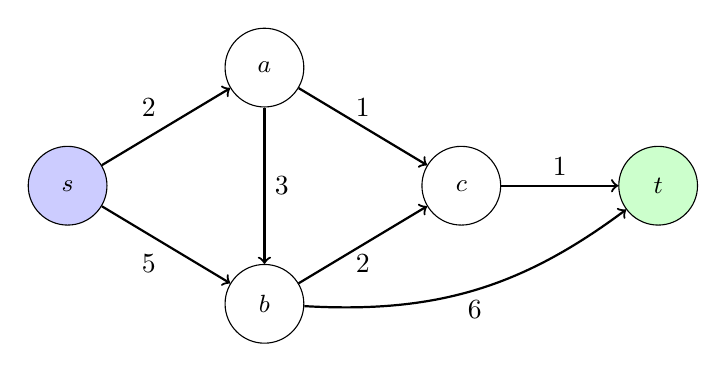
\begin{tikzpicture}[
    node distance=2.5cm,
    vertex/.style={circle, draw, minimum size=10mm, font=\small},
    edge/.style={->, thick}
]
    % 顶点
    \node[vertex, fill=blue!20] (s) at (0,0) {$s$};
    \node[vertex] (a) at (2.5,1.5) {$a$};
    \node[vertex] (b) at (2.5,-1.5) {$b$};
    \node[vertex] (c) at (5,0) {$c$};
    \node[vertex, fill=green!20] (t) at (7.5,0) {$t$};
    
    % 边和权重
    \draw[edge] (s) -- node[above left] {$2$} (a);
    \draw[edge] (s) -- node[below left] {$5$} (b);
    \draw[edge] (a) -- node[above] {$1$} (c);
    \draw[edge] (a) -- node[right] {$3$} (b);
    \draw[edge] (b) -- node[below] {$2$} (c);
    \draw[edge] (c) -- node[above] {$1$} (t);
    \draw[edge] (b) to[bend right=20] node[below] {$6$} (t);
\end{tikzpicture}
\caption{一个简单的有向图。从$s$到$t$有多条路径，最短的是$s \to a \to c \to t$，总代价为$2+1+1=4$。}
\end{figure}

\subsection{最短路的递归结构}

设$d(v)$为从顶点$v$到终点$t$的最短距离。显然$d(t) = 0$。

对于其他顶点$v$，想一想：从$v$出发的最短路是什么样的？

你必须先走一步到某个邻居$u$，然后再从$u$走到$t$。总代价是"这一步的代价"加上"从$u$到$t$的最短距离"。而你应该选择让总代价最小的那个邻居。

用数学语言：
\begin{equation}
    d(v) = \min_{u \in \text{neighbors}(v)} \left[ w_{vu} + d(u) \right]
\end{equation}

这就是最短路问题的\textbf{贝尔曼方程}！

\begin{marginnote}
对比强化学习的贝尔曼方程$V(s) = \max_a[r + \gamma V(s')]$：
\begin{itemize}
    \item 最短路是最小化代价，RL是最大化奖励
    \item 最短路没有折扣（$\gamma = 1$）
    \item 最短路的"动作"就是选择下一个顶点
\end{itemize}
\end{marginnote}


\subsection{手工计算最短路径}

让我们逐步分析这个图，找出从 $s$ 到 $t$ 的最短路径。我们将介绍三种方法，它们体现了不同的计算思路。

\subsubsection{方法一：枚举所有路径}

对于这个小规模的图，我们可以直接枚举所有可能的路径：

\begin{enumerate}
    \item 路径 $s \to a \to c \to t$：代价 $2 + 1 + 1 = 4$
    \item 路径 $s \to b \to c \to t$：代价 $5 + 2 + 1 = 8$
    \item 路径 $s \to b \to t$：代价 $5 + 6 = 11$
    \item 路径 $s \to a \to b \to c \to t$：代价 $2 + 3 + 2 + 1 = 8$
    \item 路径 $s \to a \to b \to t$：代价 $2 + 3 + 6 = 11$
\end{enumerate}

比较可知，最短路径是 $s \to a \to c \to t$，总代价为 $4$。

枚举法虽然直观，但当图的规模增大时，路径数量会\textbf{指数级增长}，变得不可行。我们需要更聪明的方法。

\subsubsection{方法二：深度优先搜索（从终点回溯）}

深度优先搜索（Depth-First Search, DFS）的思想是：\textbf{沿着一条路径走到底，再回溯尝试其他分支}。我们从终点 $t$ 出发，逆向计算每个节点的最短距离。

定义 $V(x)$ 为从顶点 $x$ 到终点 $t$ 的最短距离。计算过程如下：

\begin{enumerate}
    \item \textbf{求 $V(s)$}：$s$ 有两个邻居 $a$ 和 $b$，需要先知道 $V(a)$ 和 $V(b)$
    
    \item \textbf{递归求 $V(a)$}：$a$ 有两个邻居 $c$ 和 $b$，需要先知道 $V(c)$ 和 $V(b)$
    
    \item \textbf{递归求 $V(c)$}：$c$ 只有一个邻居 $t$
    \[
        V(c) = w(c,t) + V(t) = 1 + 0 = 1 \quad \checkmark
    \]
    
    \item \textbf{递归求 $V(b)$}（从 $a$ 的分支触发）：$b$ 有两个邻居 $c$ 和 $t$
    \[
        V(b) = \min\{w(b,c) + V(c), \; w(b,t) + V(t)\} = \min\{2+1, \; 6+0\} = 3 \quad \checkmark
    \]
    
    \item \textbf{回到 $V(a)$}：现在 $V(c)=1$，$V(b)=3$ 都已知
    \[
        V(a) = \min\{w(a,c) + V(c), \; w(a,b) + V(b)\} = \min\{1+1, \; 3+3\} = 2 \quad \checkmark
    \]
    
    \item \textbf{回到 $V(s)$}：现在 $V(a)=2$，$V(b)=3$ 都已知
    \[
        V(s) = \min\{w(s,a) + V(a), \; w(s,b) + V(b)\} = \min\{2+2, \; 5+3\} = 4 \quad \checkmark
    \]
\end{enumerate}

图 \ref{fig:dfs-tree} 展示了这个递归调用的过程。

\begin{figure}[h]
\centering
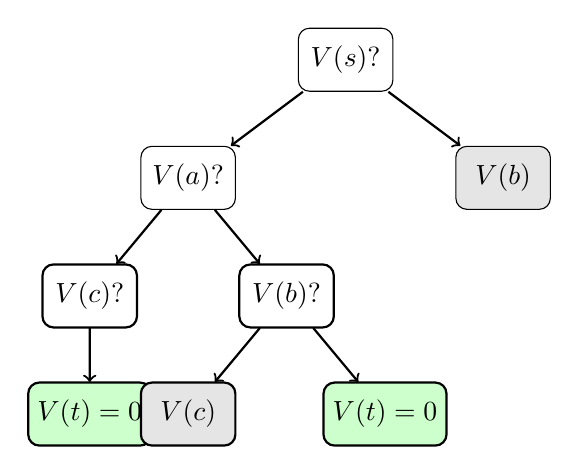
\begin{tikzpicture}[
    level distance=1.5cm,
    sibling distance=3cm,
    every node/.style={draw, rounded corners, minimum width=1.2cm, minimum height=0.8cm},
    edge from parent/.style={draw, ->, thick},
    level 1/.style={sibling distance=4cm},
    level 2/.style={sibling distance=2.5cm}
]
    \node {$V(s)$?}
        child {node {$V(a)$?}
            child {node {$V(c)$?}
                child {node[fill=green!20] {$V(t)=0$}}
            }
            child {node {$V(b)$?}
                child {node[fill=gray!20] {$V(c)$}}
                child {node[fill=green!20] {$V(t)=0$}}
            }
        }
        child {node[fill=gray!20] {$V(b)$}};
\end{tikzpicture}
\caption{深度优先搜索的递归调用树。灰色节点表示已经计算过，可以直接返回缓存结果（这就是\textbf{记忆化}）。}
\label{fig:dfs-tree}
\end{figure}

\begin{remark}
注意到 $V(b)$ 被请求了两次（一次从 $a$，一次从 $s$），但我们只需要计算一次，第二次直接返回缓存的结果。这种技术叫做\textbf{记忆化}（memoization），它把朴素递归的指数时间复杂度降低到多项式时间。
\end{remark}

\subsubsection{方法三：广度优先/逐层更新（Bellman-Ford 风格）}

另一种思路是\textbf{逐层更新}：不是沿着一条路径走到底，而是每一轮同时更新所有节点的估计值，直到收敛。

初始化：$V^{(0)}(t) = 0$，其他节点 $V^{(0)}(x) = \infty$。

\textbf{第 1 轮更新}：考虑所有能一步到达 $t$ 的节点
\begin{align*}
    V^{(1)}(c) &= w(c,t) + V^{(0)}(t) = 1 + 0 = 1 \\
    V^{(1)}(b) &= w(b,t) + V^{(0)}(t) = 6 + 0 = 6
\end{align*}

\textbf{第 2 轮更新}：基于第 1 轮的结果继续更新
\begin{align*}
    V^{(2)}(a) &= \min\{w(a,c) + V^{(1)}(c), \; w(a,b) + V^{(1)}(b)\} = \min\{1+1, \; 3+6\} = 2 \\
    V^{(2)}(b) &= \min\{V^{(1)}(b), \; w(b,c) + V^{(1)}(c)\} = \min\{6, \; 2+1\} = 3 \quad \text{（更新！）}
\end{align*}

\textbf{第 3 轮更新}：
\begin{align*}
    V^{(3)}(s) &= \min\{w(s,a) + V^{(2)}(a), \; w(s,b) + V^{(2)}(b)\} = \min\{2+2, \; 5+3\} = 4
\end{align*}

第 4 轮更新后所有值不再变化，算法收敛。

\begin{table}[h]
\centering
\begin{tabular}{c|ccccc}
\toprule
轮次 & $V(s)$ & $V(a)$ & $V(b)$ & $V(c)$ & $V(t)$ \\
\midrule
初始 & $\infty$ & $\infty$ & $\infty$ & $\infty$ & $0$ \\
第 1 轮 & $\infty$ & $\infty$ & $6$ & $1$ & $0$ \\
第 2 轮 & $\infty$ & $2$ & $3$ & $1$ & $0$ \\
第 3 轮 & $4$ & $2$ & $3$ & $1$ & $0$ \\
\bottomrule
\end{tabular}
\caption{广度优先/逐层更新的迭代过程}
\end{table}

\subsubsection{两种策略的比较}

上述两种方法对应了求解贝尔曼方程的两种基本策略：

\begin{table}[h]
\centering
\begin{tabular}{lll}
\toprule
\textbf{特性} & \textbf{深度优先（DFS）} & \textbf{广度优先/逐层更新} \\
\midrule
计算顺序 & 沿路径深入，遇到未知再递归 & 每轮同时更新所有节点 \\
核心技术 & 递归 + 记忆化 & 迭代 + 值更新 \\
典型算法 & 记忆化搜索、策略迭代 & Bellman-Ford、值迭代 \\
适用场景 & 状态空间稀疏、只需部分解 & 状态空间稠密、需要全局解 \\
\bottomrule
\end{tabular}
\caption{深度优先与广度优先策略的比较}
\end{table}

\begin{figure}[h]
\centering
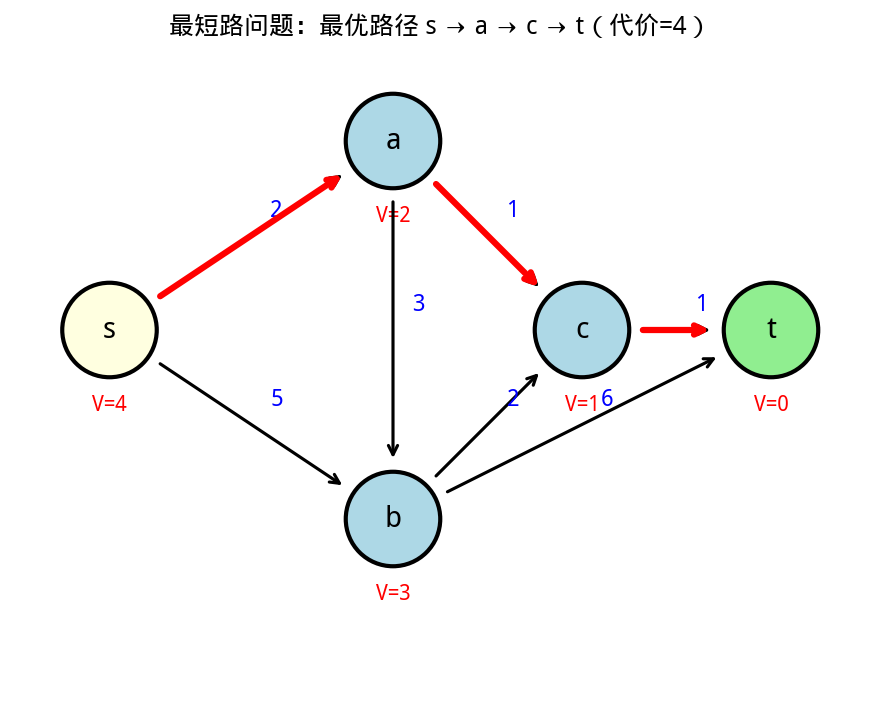
\includegraphics[width=0.6\textwidth]{figs/chap10_shortest_path.png}
\caption{最短路问题示意图。红色箭头标示最优路径$s \to a \to c \to t$，总代价为4。每个节点旁标注的$V$值是从该点到终点的最短距离。}
\label{fig:shortest_path}
\end{figure}

\subsection{最短路的线性规划形式}

最短路问题可以写成一个优雅的\textbf{线性规划}。这个视角将帮助我们深入理解求解算法的本质。

\subsubsection{原始问题：流量视角}

想象每条边上有"流量"$x_{ij}$。我们要把一单位的流量从$s$送到$t$，使得总代价最小：

\begin{equation}
    \begin{aligned}
        \min_{x} \quad & \sum_{(i,j) \in E} w_{ij} \cdot x_{ij} \\
        \text{s.t.} \quad & \sum_{j} x_{ij} - \sum_{k} x_{ki} = \begin{cases}
            1 & \text{if } i = s \\
            -1 & \text{if } i = t \\
            0 & \text{otherwise}
        \end{cases} \\
        & x_{ij} \geq 0, \quad \forall (i,j) \in E
    \end{aligned}
\end{equation}

这里的约束叫做\textbf{流量守恒}：除了起点（流出1单位）和终点（流入1单位），其他每个顶点流入等于流出。

\subsubsection{对偶问题：势能视角}

现在我们来写这个线性规划的对偶问题。

为每个顶点 $i$ 的流量守恒约束引入对偶变量 $V_i$（你可以把它想象成顶点的"势能"或"位置"）。根据线性规划对偶理论，对偶问题是：

\begin{keyformula}[title=最短路的对偶问题]
\begin{equation}
    \begin{aligned}
        \max_{V} \quad & V_t - V_s \\
        \text{s.t.} \quad & V_j - V_i \leq w_{ij}, \quad \forall (i,j) \in E
    \end{aligned}
\end{equation}
\end{keyformula}

\paragraph{物理直觉：绳网模型}

这个对偶问题有一个美妙的物理解释。想象每条边 $(i,j)$ 是一根\textbf{长度为 $w_{ij}$ 的绳子}，连接顶点 $i$ 和 $j$。现在：

\begin{itemize}
    \item 把起点 $s$ 固定在左边的墙壁上
    \item 把终点 $t$ 尽可能向右拉
    \item 绳子不能被拉断——相邻顶点的水平距离不能超过绳长
\end{itemize}

你能把 $t$ 拉到离墙多远？答案正是从 $s$ 到 $t$ 的最短路长度！

\begin{figure}[h]
\centering
\begin{tikzpicture}[scale=1.1]
    % 距离标尺
    \draw[->] (0,-3) -- (8.5,-3) node[right] {势能 $V$};
    \foreach \x in {0,1,2,3,4} {
        \draw (\x*2,-3.1) -- (\x*2,-2.9) node[below=2pt] {\small \x};
    }
    
    % 松弛的绳子（用抛物线/悬链线表示下垂）
    % s -> b: 绳长5，水平距离1，大量松弛
    \draw[thick, blue!60, decorate, decoration={snake, amplitude=0pt}] 
        (0,0) .. controls (0.5,-1.5) and (1.5,-2) .. (2,-1.5);
    \node[blue!60] at (0.6,-1.3) {\small $w=5$};
    
    % a -> b: 绳长3，松弛
    \draw[thick, blue!60] 
        (4,0) .. controls (3.5,-0.8) and (2.5,-1.2) .. (2,-1.5);
    \node[blue!60] at (2.7,-0.6) {\small $w=3$};
    
    % b -> c: 绳长2，水平距离2，轻微松弛
    \draw[thick, blue!60] 
        (2,-1.5) .. controls (3,-1.8) and (5,-0.8) .. (6,0);
    \node[blue!60] at (4,-1.5) {\small $w=2$};
    
    % b -> t: 绳长6，水平距离3，大量松弛
    \draw[thick, blue!60] 
        (2,-1.5) .. controls (4,-2.5) and (6,-1.5) .. (8,0);
    \node[blue!60] at (5.5,-2.3) {\small $w=6$};
    
    % 顶点（先画顶点，再画线和标签，确保标签在最上层）
    \node[circle, draw, fill=blue!20, minimum size=10mm] (s) at (0,0) {$s$};
    \node[circle, draw, fill=white, minimum size=10mm] (a) at (4,0) {$a$};
    \node[circle, draw, fill=white, minimum size=10mm] (b) at (2,-1.5) {$b$};
    \node[circle, draw, fill=white, minimum size=10mm] (c) at (6,0) {$c$};
    \node[circle, draw, fill=green!20, minimum size=10mm] (t) at (8,0) {$t$};

    % 拉紧的绳子（水平直线）- 最短路径，在节点之间
    \draw[red, very thick] (s.east) -- (a.west);
    \draw[red, very thick] (a.east) -- (c.west);
    \draw[red, very thick] (c.east) -- (t.west);

    % 拉紧标签（放在线的上方，避开节点）
    \node[red, fill=white, inner sep=1pt] at (2,0.25) {\scriptsize $w=2$};
    \node[red, fill=white, inner sep=1pt] at (5,0.25) {\scriptsize $w=1$};
    \node[red, fill=white, inner sep=1pt] at (7,0.25) {\scriptsize $w=1$};
    
    % 势能标注
    \node[above] at (0,0.6) {$V_s = 0$};
    \node[above] at (4,0.6) {$V_a = 2$};
    \node[below] at (2,-2.1) {$V_b = 1$};
    \node[above] at (6,0.6) {$V_c = 3$};
    \node[above] at (8,0.6) {$V_t = 4$};
    
    % 固定墙壁（左）
    \fill[gray!40] (-0.8,-2.5) rectangle (-0.5,1.5);
    \draw[thick] (-0.5,-2.5) -- (-0.5,1.5);
    \foreach \y in {-2,-1.5,...,1} {
        \draw[thick] (-0.8,\y) -- (-0.5,\y+0.3);
    }
    
    % 固定点
    \draw[thick] (-0.5,0) -- (0,0);
    \node[left] at (-0.8,0) {\small 固定};
    
    % 向右拉的箭头
    \draw[->, very thick, red!70] (8.6,0) -- (9.4,0) node[right] {拉！};
    
\end{tikzpicture}
\caption{绳网模型：把 $s$ 固定在墙壁，向右拉 $t$。红色的边被完全拉紧成水平直线，构成最短路径 $s \to a \to c \to t$。蓝色的边是松弛的，自然下垂。$t$ 到墙壁的水平距离（$4$）就是最短路长度。}
\label{fig:rope-network}
\end{figure}

\paragraph{为什么这是对的？}

\begin{itemize}
    \item \textbf{约束 $V_j - V_i \leq w_{ij}$}：绳子的长度限制。如果 $j$ 比 $i$ 向右超出绳长 $w_{ij}$，绳子就会被拉断。
    
    \item \textbf{目标 $\max(V_t - V_s)$}：我们想把 $t$ 拉得尽可能远离墙壁。
    
    \item \textbf{最优解}：当我们把 $t$ 拉到极限时，从 $s$ 到 $t$ 必有一条"全部拉紧"的路径——沿着这条路径，每根绳子都水平绑紧，即 $V_j - V_i = w_{ij}$。把这些等式沿路径相加：
    \[
        V_t - V_s = \sum_{\text{路径上的边}} w_{ij}
    \]
    这正是路径的总长度！而且因为其他路径的绳子在下垂（没拉紧），这条路径一定是最短的。
\end{itemize}

\begin{remark}
这个绳网模型揭示了最短路问题的\textbf{对偶结构}：
\begin{itemize}
    \item \textbf{原问题}（流的视角）：寻找从 $s$ 到 $t$ 的最小代价流
    \item \textbf{对偶问题}（势能视角）：寻找满足"绳长约束"的最大水平距离
\end{itemize}
强对偶定理告诉我们：最小流量代价 $=$ 最大势能差。这个等式在图 \ref{fig:rope-network} 中的体现是：$t$ 能被拉到的距离（$4$）恰好等于最短路的长度（$4$）。
\end{remark}

\paragraph{紧致条件与最短路径}

在最优解中，哪些边的约束取等号（$V_j - V_i = w_{ij}$）？正是\textbf{最短路径上的边}！

这些边在图中被完全拉成水平直线——水平距离恰好等于绳长。回到我们的例子：
\begin{align*}
    V_a - V_s &= 2 - 0 = 2 = w_{sa} \quad \text{（水平拉紧 }\checkmark\text{）} \\
    V_c - V_a &= 3 - 2 = 1 = w_{ac} \quad \text{（水平拉紧 }\checkmark\text{）} \\
    V_t - V_c &= 4 - 3 = 1 = w_{ct} \quad \text{（水平拉紧 }\checkmark\text{）}
\end{align*}

而非最短路径上的边则是松弛下垂的：
\begin{align*}
    V_b - V_s &= 1 - 0 = 1 < 5 = w_{sb} \quad \text{（下垂，剩余长度 $4$）} \\
    V_t - V_b &= 4 - 1 = 3 < 6 = w_{bt} \quad \text{（下垂，剩余长度 $3$）}
\end{align*}

这给了我们一个识别最短路径的方法：找到那些被水平拉紧的边，它们串起来就是最短路径。

\begin{remark}
松弛变量的物理意义也很清楚：它是绳子的\textbf{下垂量}（更准确地说，是绳长减去水平投影的差值）。绳子下垂得越厉害，说明这条边离"最短路"越远。如果 $V_b - V_s = 1$ 而 $w_{sb} = 5$，说明这根绳子还可以再水平拉伸 $4$ 个单位才会绑紧——这告诉我们走 $s \to b$ 这条路，后面还需要额外 $4$ 的代价才能"追上"最短路径。
\end{remark}
% ------------------------------------------------------------------------------------
\section{两种求解思路：对偶上升与原始改进}
% ------------------------------------------------------------------------------------

现在我们有了最短路问题的原始-对偶结构。如何求解？

有两种根本不同的策略，它们对应着你可能听说过的两类算法。

\subsection{策略一：对偶上升——维护最优性}

\textbf{核心思想}：从势能函数$V$出发，始终保持$V$满足所有约束（对偶可行），逐步提升目标$V_t - V_s$。

想象你是一个"保守派"：你不愿意冒险，每一步都要确保自己的解是"合法"的。

具体做法：
\begin{enumerate}
    \item 初始化：$V_t = 0$，其他$V_i = -\infty$（或者某个很小的值）
    \item 找到一个可以"提升"的顶点：存在边$(i,j)$使得$V_i < V_j - w_{ij}$
    \item 更新：$V_i \leftarrow V_j - w_{ij}$（让约束紧绑）
    \item 重复，直到无法再提升
\end{enumerate}

\textbf{关键性质}：每次更新都让$V_s$变大（因为势能像波浪一样从$t$向$s$传播），而且每一步的$V$都满足所有约束。

这就是\textbf{Dijkstra算法}的本质！它从终点开始，像水波一样向外扩展势能等值面。

\begin{figure}[h]
\centering
\begin{tikzpicture}[scale=0.9]
    % 波纹
    \fill[blue!10] (0,0) circle (2.5);
    \fill[blue!20] (0,0) circle (1.8);
    \fill[blue!30] (0,0) circle (1.1);
    \fill[blue!50] (0,0) circle (0.4);
    
    \node[font=\small] at (0,0) {$t$};
    \node[font=\footnotesize] at (0.8,0.8) {$V=1$};
    \node[font=\footnotesize] at (1.4,1.4) {$V=2$};
    \node[font=\footnotesize] at (2,2) {$V=3$};
    
    \node[below, font=\small] at (0,-3) {势能等值面从终点向外扩展};
\end{tikzpicture}
\caption{Dijkstra算法的几何直观：对偶上升}
\end{figure}

\subsection{策略二：原始改进——维护可行性}

\textbf{核心思想}：从一条实际路径出发，始终保持有一条从$s$到$t$的路（原始可行），逐步缩短路径长度。

想象你是一个"冒险家"：你先冲到终点再说，然后慢慢优化路线。

具体做法：
\begin{enumerate}
    \item 随便找一条从$s$到$t$的路径（可能很绕）
    \item 检查：有没有"捷径"可以替换当前路径的某一段？
    \item 如果有，更新路径
    \item 重复，直到找不到更短的路
\end{enumerate}

\textbf{关键性质}：每次更新都让路径变短，而且每一步都有一条完整的可行路径。

这就是\textbf{Bellman-Ford算法}的精神！它通过反复"松弛"所有边，让最短距离信息逐渐传播。

\subsection{两种策略的对比}

\begin{table}[h]
\centering
\caption{对偶上升 vs 原始改进}
\begin{tabular}{lcc}
\toprule
& \textbf{对偶上升（Dijkstra风格）} & \textbf{原始改进（Bellman-Ford风格）} \\
\midrule
维护什么 & 势能函数$V$（对偶变量） & 具体路径（原始变量） \\
解的状态 & 对偶可行，但可能"不完整" & 原始可行，但可能"不最优" \\
每步做什么 & 扩展确定区域 & 改进当前路径 \\
收敛时 & 对偶目标达到最优 & 原始目标达到最优 \\
界的变化 & 下界$\uparrow$上升 & 上界$\downarrow$下降 \\
\midrule
适用条件 & 需要边权非负 & 允许负边权 \\
时间复杂度 & $O(E \log V)$ & $O(VE)$ \\
\bottomrule
\end{tabular}
\end{table}

\begin{physicalmeaning}
\textbf{选择哪种策略？}

这取决于你的问题结构：
\begin{itemize}
    \item 如果约束容易满足，但找最优解难——用\textbf{对偶上升}（先保证最优，再扩展可行域）
    \item 如果找最优解容易，但满足约束难——用\textbf{原始改进}（先保证可行，再改进目标）
\end{itemize}

在最短路问题中，找一条路（原始可行）很容易，但要找最短的那条（最优）较难，所以Dijkstra（对偶上升）通常更高效。
\end{physicalmeaning}

% ------------------------------------------------------------------------------------
\section{从最短路到强化学习：算法设计的核心权衡}
% ------------------------------------------------------------------------------------

在最短路问题中，我们见识了两种截然不同的求解思路：
\begin{itemize}
    \item \textbf{深度优先}：沿着一条路走到底，看看总代价是多少，再回溯尝试其他路径
    \item \textbf{动态规划}：从终点往回推，逐步计算每个节点的最优值
\end{itemize}

这两种思路的差异，其实反映了算法设计中一个根本性的权衡。当我们从最短路走向更复杂的强化学习问题时，这个权衡会变得更加关键，同时还会出现新的挑战。

本节我们将建立一个"算法坐标系"，帮助你理解各种强化学习算法的设计逻辑。

% ------------------------------------------------------------------------------------
\subsection{核心权衡：探索深度 vs. 计算代价}
% ------------------------------------------------------------------------------------

让我们先聚焦于两个最基本的维度：\textbf{我们要探索多深}，以及\textbf{我们对环境了解多少}。

\subsubsection{维度一：更新深度——走多远再回头？}

\begin{keyidea}[title=核心问题]
更新价值函数时，我们应该走多少步再回头总结经验？
\end{keyidea}

回想最短路的两种算法：

\textbf{深度优先搜索}必须走完一整条路径才能知道这条路的代价。如果路径很长，中间有很多岔路，每条岔路又有岔路……搜索空间会指数爆炸。

\textbf{动态规划}则聪明得多：它只看"一步"。从终点开始，先算出离终点一步的节点的最优值；再算离终点两步的；依此类推。每一步都利用之前算好的结果，避免了重复计算。

这两种思路在强化学习中分别对应：

\paragraph{蒙特卡洛方法（MC）——"走到底再算账"}

就像深度优先搜索，MC方法必须完成一整个\textbf{回合}（episode），才能计算这条轨迹的总回报：
\begin{equation}
    G_t = r_t + \gamma r_{t+1} + \gamma^2 r_{t+2} + \cdots + \gamma^{T-t} r_T
\end{equation}

\paragraph{时序差分方法（TD）——"走一步就更新"}

就像动态规划，TD方法只看一步，然后用对下一状态的\textbf{估计值}来补全剩余部分：
\begin{equation}
    \text{TD目标} = r_t + \gamma \hat{V}(s_{t+1})
\end{equation}

这种"用估计更新估计"的技巧叫做\textbf{自举}（Bootstrapping）——就像拽着自己的鞋带把自己提起来。

\paragraph{直观理解：期中考 vs. 期末考}

假设你是老师，想预测学生的学习效果：

\begin{itemize}
    \item \textbf{TD思路}：期中考完就预测期末成绩。反馈快，但可能不准（有\textbf{偏差}）。
    \item \textbf{MC思路}：等期末考完再看真实成绩。绝对准确（\textbf{无偏}），但如果学生那天生病或超常发挥，结果波动很大（高\textbf{方差}）。
\end{itemize}

\begin{figure}[h]
\centering
\begin{tikzpicture}[scale=0.85, >=stealth]
    % 时间轴
    \draw[->, thick] (0,0) -- (14,0) node[right] {时间};
    
    % 状态节点
    \foreach \i/\label in {0/$s_t$, 2.5/$s_{t+1}$, 5/$s_{t+2}$, 9/$s_{t+3}$, 12.5/终点} {
        \fill (\i, 0) circle (3pt);
        \node[below] at (\i, -0.3) {\label};
    }
    \node at (7, 0) {$\cdots$};
    \node at (11, 0) {$\cdots$};
    
    % 奖励
    \foreach \i/\r in {1.25/$r_t$, 3.75/$r_{t+1}$, 6/$r_{t+2}$} {
        \node[above, blue] at (\i, 0.3) {\small \r};
    }
    
    % TD(0)：只看一步
    \draw[red, very thick, ->] (0, 1.2) -- (2.5, 1.2);
    \node[red, above] at (1.25, 1.2) {\textbf{TD(0)}};
    \node[red, right, font=\small] at (2.7, 1.2) {$r_t + \gamma \hat{V}(s_{t+1})$};
    \draw[red, dashed] (2.5, 1) -- (2.5, 0.2);
    
    % n-step
    \draw[orange, very thick, ->] (0, 2.2) -- (5, 2.2);
    \node[orange, above] at (2.5, 2.2) {\textbf{n-step TD}};
    \draw[orange, dashed] (5, 2) -- (5, 0.2);
    
    % MC：走到底
    \draw[green!60!black, very thick, ->] (0, 3.2) -- (12.5, 3.2);
    \node[green!60!black, above] at (6.25, 3.2) {\textbf{Monte Carlo}};
    \node[green!60!black, right, font=\small] at (12.7, 3.2) {$G_t = \sum \gamma^k r_{t+k}$};
    
\end{tikzpicture}
\caption{不同的更新深度：TD只看一步，n-step看若干步，MC走到终点}
\end{figure}

\subsubsection{维度二：模型依赖——能不能"想象"？}

\begin{keyidea}[title=核心问题]
我们知道环境的运作规则吗？能在脑中"推演"吗？
\end{keyidea}

回想最短路问题：我们知道图的完整结构——哪些节点相连、每条边的权重。有了这些信息，动态规划才能施展威力。

但如果你\textbf{不知道}图的结构呢？你只能从起点出发，走一步看一步，通过不断试错来摸清地形。

这就是\textbf{有模型}与\textbf{无模型}的区别：

\paragraph{有模型方法（Model-based）}

你知道（或者学会了）环境的"规则"：
\begin{itemize}
    \item 状态转移：从状态 $s$ 采取动作 $a$，会到达什么状态 $s'$？
    \item 奖励函数：这一步能获得多少奖励？
\end{itemize}

有了模型，你可以在"脑海中"推演，不需要真的和环境交互。就像下棋高手，不需要真的落子，就能在脑中预判十几步之后的局面。

\paragraph{无模型方法（Model-free）}

你对环境一无所知，只能通过\textbf{真实的试错}来学习。每次想知道某个动作好不好，都必须真的去做，承受后果。

\begin{table}[h]
\centering
\renewcommand{\arraystretch}{1.4}
\begin{tabular}{p{2.5cm}|p{5.5cm}|p{5.5cm}}
\toprule
& \textbf{有模型 (Model-based)} & \textbf{无模型 (Model-free)} \\
\midrule
\textbf{类比} & 知道棋盘规则，脑中推演 & 不知规则，只能试错 \\
\midrule
\textbf{优势} & 
数据效率极高；可以"想象"从未经历的情况；可以谨慎避免危险
 & 
实现简单；不怕模型不准；渐进性能通常更好
 \\
\midrule
\textbf{劣势} & 
模型难以精确获得；模型偏差会导致策略失效
 & 
需要海量真实交互；每次学习都要真的"摔跤"
 \\
\midrule
\textbf{代表算法} & AlphaZero、MuZero、Dreamer & DQN、PPO、SAC \\
\bottomrule
\end{tabular}
\caption{有模型 vs. 无模型方法的对比}
\end{table}

\subsubsection{二维图谱：算法的基本定位}

现在我们可以用这两个维度画出一张"算法地图"：

\begin{figure}[h]
\centering
\begin{tikzpicture}[scale=1.15, >=stealth]
    % 坐标轴
    \draw[->, very thick] (-5.2,0) -- (5.2,0);
    \draw[->, very thick] (0,-3.5) -- (0,3.8);
    
    % 轴标签
    \node[above] at (0, 3.8) {\textbf{模型依赖}};
    \node[right] at (5.2, 0) {\textbf{更新深度}};
    
    \node[below, font=\small, align=center] at (-4,0) {深 (MC)\\ \scriptsize 无偏·高方差};
    \node[below, font=\small, align=center] at (4,0) {浅 (TD)\\ \scriptsize 有偏·低方差};
    \node[left, font=\small, align=right] at (0,3) {有模型\\ \scriptsize 可以规划};
    \node[left, font=\small, align=right] at (0,-3) {无模型\\ \scriptsize 只能试错};
    
    % --- 四个象限 ---
    
    % 右上：动态规划
    \node[draw=blue!80, thick, rounded corners, fill=blue!10, text width=3cm, align=center] at (3.3, 2.3) {
        \textbf{动态规划}\\[3pt]
        \footnotesize Value Iteration\\
        Policy Iteration\\[3pt]
        \scriptsize 理论最优解
    };
    
    % 左上：规划搜索
    \node[draw=green!60!black, thick, rounded corners, fill=green!10, text width=3cm, align=center] at (-3.3, 2.3) {
        \textbf{树搜索}\\[3pt]
        \footnotesize MCTS\\
        AlphaZero\\[3pt]
        \scriptsize 围棋、国际象棋
    };
    
    % 左下：蒙特卡洛RL
    \node[draw=red!80, thick, rounded corners, fill=red!10, text width=3cm, align=center] at (-3.3, -2.3) {
        \textbf{蒙特卡洛 RL}\\[3pt]
        \footnotesize REINFORCE\\
        GRPO\\[3pt]
        \scriptsize 大模型训练
    };
    
    % 右下：时序差分RL
    \node[draw=orange!80, thick, rounded corners, fill=orange!10, text width=3cm, align=center] at (3.3, -2.3) {
        \textbf{时序差分 RL}\\[3pt]
        \footnotesize Q-Learning, DQN\\
        SARSA\\[3pt]
        \scriptsize 游戏AI
    };
    
    % 中间：Actor-Critic
    \node[draw=purple!80, thick, dashed, rounded corners, fill=purple!10, text width=3.2cm, align=center] at (0, -2.3) {
        \textbf{Actor-Critic}\\[3pt]
        \footnotesize PPO, SAC, A3C\\[3pt]
        \scriptsize 工业界主流
    };
    
    % 连接线
    \draw[dashed, gray] (-1.6, -2.3) -- (-3.3+1.5, -2.3);
    \draw[dashed, gray] (1.6, -2.3) -- (3.3-1.5, -2.3);
    
    % 对角线箭头表示权衡
    \draw[->, thick, gray, dashed] (-3.5, -3) -- (3.5, 3) node[pos=0.85, above, sloped, font=\small] {单步计算代价 $\uparrow$};
    
\end{tikzpicture}
\caption{强化学习算法的基本图谱。横轴是更新深度，纵轴是模型依赖程度。对角线方向代表计算代价的增加。}
\label{fig:rl-2d-map}
\end{figure}

\paragraph{图谱解读}

\begin{itemize}
    \item \textbf{右上角（动态规划）}：最短路问题就在这里！我们知道完整的图结构（有模型），用自举更新（TD式）。这是理论上最理想的情况——如果你能准确描述环境，动态规划给出的就是最优解。
    
    \item \textbf{左上角（树搜索）}：AlphaZero在这里。它知道棋盘规则（有模型），通过蒙特卡洛树搜索（MCTS）进行深度推演。计算量大，但效果惊人。
    
    \item \textbf{右下角（时序差分RL）}：DQN、Q-Learning在这里。不知道环境规则（无模型），只能通过试错学习，但每一步都及时更新（TD），收敛相对较快。
    
    \item \textbf{左下角（蒙特卡洛RL）}：REINFORCE、GRPO在这里。不知道模型，还必须走完整条轨迹才能更新。听起来最"笨"，但在某些场景下（如大语言模型训练）反而有独特优势。
    
    \item \textbf{中央（Actor-Critic）}：PPO、SAC等算法介于TD和MC之间，是目前工业界最常用的方法。
\end{itemize}

\begin{remark}
注意对角线方向：从右下到左上，计算代价递增。无模型+浅层更新单步最"便宜"；有模型+深度搜索单步最"昂贵"但也最强大。选择算法时，需要根据问题特点和计算预算来权衡。
\end{remark}

% ------------------------------------------------------------------------------------
\subsection{两个关键因素：数据的来源与使用}
% ------------------------------------------------------------------------------------

上面的二维图谱描述了"怎么计算"的问题。但在实际应用中，还有另一个同样重要的问题：\textbf{数据从哪来、怎么用}？

这涉及两个额外的维度，它们决定了算法的\textbf{数据效率}和\textbf{适用场景}。

\subsubsection{维度三：数据新鲜度（On-policy vs. Off-policy）}

\begin{keyidea}[title=核心问题]
训练数据必须来自当前策略吗？能不能用"过时"的数据？
\end{keyidea}

\paragraph{类比：学游泳}

你现在的游泳姿势是A，游了一圈后，教练给你反馈，你调整成姿势B。

问题来了：\textbf{刚才用姿势A游的那一圈数据，还能用来改进姿势B吗？}

\begin{itemize}
    \item \textbf{On-policy（同策略）}：不能。姿势A和姿势B的水感不同，旧数据可能产生误导。每次更新后，旧数据必须丢弃。
    
    \item \textbf{Off-policy（异策略）}：可以！通过数学技巧（如重要性采样），我们可以"修正"旧数据，使其对新策略也有参考价值。
\end{itemize}

\begin{figure}[h]
\centering
\begin{tikzpicture}[scale=0.85, >=stealth]
    % On-policy
    \begin{scope}[xshift=-5cm]
        \node[font=\bfseries] at (0, 3.2) {On-policy};
        \node[font=\small, gray] at (0, 2.7) {"数据保鲜期：一次"};
        
        \node[draw, rounded corners, fill=blue!20, minimum width=2cm, minimum height=0.7cm] (pi) at (0, 1.8) {策略 $\pi_\theta$};
        \node[draw, rounded corners, fill=green!20, minimum width=2cm, minimum height=0.7cm] (env) at (0, 0) {环境};
        \node[draw, rounded corners, fill=orange!20, minimum width=1.4cm, minimum height=0.5cm] (data) at (2.5, 0.9) {\small 数据};
        
        \draw[->, thick] (pi) -- node[left, font=\small] {交互} (env);
        \draw[->, thick] (env) -- (data);
        \draw[->, thick] (data) -- node[above, font=\small] {更新} (pi);
        
        \node[draw, rounded corners, fill=red!15, font=\small] at (2.5, -0.5) {丢弃};
        \draw[->, thick, red] (data) -- (2.5, -0.1);
    \end{scope}
    
    % Off-policy
    \begin{scope}[xshift=5cm]
        \node[font=\bfseries] at (0, 3.2) {Off-policy};
        \node[font=\small, gray] at (0, 2.7) {"数据可以反复使用"};
        
        \node[draw, rounded corners, fill=blue!20, minimum width=2cm, minimum height=0.7cm] (pi2) at (0, 1.8) {策略 $\pi_\theta$};
        \node[draw, rounded corners, fill=green!20, minimum width=2cm, minimum height=0.7cm] (env2) at (0, 0) {环境};
        \node[draw, rounded corners, fill=yellow!30, minimum width=1.8cm, minimum height=1cm] (buffer) at (2.8, 0.9) {\small 经验池};
        
        \draw[->, thick] (pi2) -- node[left, font=\small] {交互} (env2);
        \draw[->, thick] (env2) -- (buffer);
        \draw[->, thick] (buffer) -- node[above, font=\small] {采样} (pi2);
        
        \draw[->, thick, green!60!black] (buffer.south) arc (-90:180:0.25) -- (buffer.west);
        \node[green!60!black, font=\scriptsize] at (1.8, -0.1) {保留};
    \end{scope}
\end{tikzpicture}
\caption{On-policy每次更新后丢弃数据，Off-policy把数据存入经验池反复使用}
\end{figure}

\begin{table}[h]
\centering
\renewcommand{\arraystretch}{1.3}
\begin{tabular}{p{2.5cm}|p{5.2cm}|p{5.2cm}}
\toprule
& \textbf{On-policy} & \textbf{Off-policy} \\
\midrule
\textbf{数据要求} & 必须是当前策略产生的 & 可以是任意策略产生的 \\
\textbf{数据利用} & 用一次就丢弃 & 存入经验池，反复使用 \\
\textbf{优势} & 理论简洁，训练稳定 & 数据效率高 \\
\textbf{劣势} & 浪费数据 & 需要额外技巧保证稳定 \\
\textbf{代表} & PPO, REINFORCE, GRPO & DQN, SAC, TD3 \\
\bottomrule
\end{tabular}
\caption{On-policy vs. Off-policy}
\end{table}

\subsubsection{维度四：交互模式（Online vs. Offline）}

\begin{keyidea}[title=核心问题]
训练时能不能和环境实时交互？还是只能用已有的历史数据？
\end{keyidea}

这个维度在大模型时代变得尤为重要。

\paragraph{类比：学开车}

\begin{itemize}
    \item \textbf{Online（在线学习）}：你坐在真车里，边开边学。教练随时给反馈，你随时调整。
    
    \item \textbf{Offline（离线学习）}：你不能碰车。只能看一大堆别人的行车记录视频，从中学习。
\end{itemize}

\begin{figure}[h]
\centering
\begin{tikzpicture}[scale=0.85, >=stealth]
    % Online
    \begin{scope}[xshift=-5cm]
        \node[font=\bfseries] at (0, 2.8) {Online};
        \node[font=\small, gray] at (0, 2.3) {"边做边学"};
        
        \node[draw, rounded corners, fill=blue!20, minimum width=2cm, minimum height=0.7cm] (agent) at (0, 1.2) {智能体};
        \node[draw, rounded corners, fill=green!20, minimum width=2cm, minimum height=0.7cm] (env) at (0, -0.8) {环境};
        
        \draw[->, thick] (agent.south west) -- node[left, font=\small] {动作} (env.north west);
        \draw[->, thick] (env.north east) -- node[right, font=\small] {反馈} (agent.south east);
        
        \node[font=\scriptsize, gray] at (0, -1.8) {可以实时交互};
    \end{scope}
    
    % Offline
    \begin{scope}[xshift=5cm]
        \node[font=\bfseries] at (0, 2.8) {Offline};
        \node[font=\small, gray] at (0, 2.3) {"只看不做"};
        
        \node[draw, rounded corners, fill=blue!20, minimum width=2cm, minimum height=0.7cm] (agent2) at (0, 1.2) {智能体};
        \node[draw, rounded corners, fill=gray!30, minimum width=2.5cm, minimum height=1cm] (data) at (0, -0.8) {\small 历史数据集};
        
        \draw[->, thick] (data) -- node[right, font=\small] {学习} (agent2);
        
        \node[draw, rounded corners, fill=green!10, minimum width=1.5cm, minimum height=0.5cm] (env2) at (3, -0.8) {\small 环境};
        \draw[thick, red] (agent2.east) -- ++(0.5,0) -- ++(0,-1.3) node[midway, right, font=\scriptsize, red] {禁止} -- (env2.north);
        \draw[red, thick] (2.2, -0.3) -- (2.6, -0.7);
        \draw[red, thick] (2.2, -0.7) -- (2.6, -0.3);
        
        \node[font=\scriptsize, gray] at (0, -2) {不能和环境交互};
    \end{scope}
\end{tikzpicture}
\caption{Online可以实时与环境交互，Offline只能从固定数据集学习}
\end{figure}

\paragraph{为什么需要Offline RL？}

在很多实际场景中，我们\textbf{无法}进行在线交互：

\begin{itemize}
    \item \textbf{医疗}：不能让AI在真实病人身上"试错"
    \item \textbf{自动驾驶}：让一辆不会开车的AI上路太危险
    \item \textbf{推荐系统}：随意推荐会损失用户和收入
    \item \textbf{大模型对齐}：每次生成都要人类标注太昂贵
\end{itemize}

但我们通常有大量的\textbf{历史数据}：过去的诊疗记录、人类司机的驾驶日志、用户的点击历史、人类写的高质量文本……

Offline RL的目标就是：\textbf{只用这些历史数据，不做任何新的交互，训练出好的策略}。

\begin{table}[h]
\centering
\renewcommand{\arraystretch}{1.3}
\begin{tabular}{p{2.5cm}|p{5.2cm}|p{5.2cm}}
\toprule
& \textbf{Online} & \textbf{Offline} \\
\midrule
\textbf{数据来源} & 实时与环境交互产生 & 固定的历史数据集 \\
\textbf{能否探索} & 可以尝试新动作 & 只能用数据中出现过的 \\
\textbf{优势} & 可以主动探索最优策略 & 安全、成本低 \\
\textbf{核心挑战} & 探索的代价（安全/成本） & 分布偏移（数据不够多样） \\
\textbf{代表} & DQN, PPO, SAC & CQL, IQL, Decision Transformer \\
\bottomrule
\end{tabular}
\caption{Online vs. Offline：交互模式的权衡}
\end{table}

\begin{example}[title=大模型训练中的Online vs. Offline]
训练ChatGPT这样的对话模型时：

\textbf{Offline阶段}：用大量人类写的文本做预训练（SFT）。这是纯Offline的——模型只是"看"人类怎么写，自己不产生任何输出。

\textbf{Online阶段}：RLHF训练时，模型生成回答，人类给反馈，模型根据反馈调整。这是Online的——模型在"边做边学"。

实际中，由于人类标注昂贵，很多工作探索如何用更少的Online交互，更多地利用Offline数据。
\end{example}

\begin{remark}
On/Off-policy 和 Online/Offline 是两个不同的维度，容易混淆：
\begin{itemize}
    \item \textbf{On/Off-policy}：问的是"数据是不是当前策略产生的"
    \item \textbf{Online/Offline}：问的是"能不能边和环境交互边训练"
\end{itemize}
一个Off-policy算法（如DQN）通常用于Online场景；而Offline RL是一个独立的研究领域，需要专门设计的算法（如CQL）。
\end{remark}

% ------------------------------------------------------------------------------------
\section{算法全景：四维定位与选择指南}
% ------------------------------------------------------------------------------------

现在我们有了四个维度，可以像GPS定位一样精确地描述任何强化学习算法。
\marginnote{\textbf{为什么DeepSeek选择MC方法？}

传统RL中MC因高方差被避免，但大模型场景有特殊性：
\begin{enumerate}
    \item 答案对错明确（如数学题）
    \item Critic网络训练成本极高
    \item 可并行采样多条轨迹降低方差
\end{enumerate}
这使"古老"的蒙特卡洛方法焕发新生。
}

\subsection{主流算法的四维属性表}

\begin{table}[htbp]
\centering
\small
\renewcommand{\arraystretch}{1.35}
\caption{主流强化学习算法的四维定位（第一部分）}
\begin{tabular}{l|c|c|c|c|p{3.5cm}}
\toprule
\textbf{算法} & \textbf{模型} & \textbf{深度} & \textbf{新鲜度} & \textbf{交互} & \textbf{典型应用} \\
\midrule
\multicolumn{6}{l}{\textit{经典基础}} \\
\midrule
Q-Learning & 无 & TD & Off-policy & Online & 理论基石 \\
SARSA & 无 & TD & On-policy & Online & Q-Learning的保守版 \\
REINFORCE & 无 & MC & On-policy & Online & 最纯粹的策略梯度 \\
\midrule
\multicolumn{6}{l}{\textit{深度强化学习}} \\
\midrule
DQN & 无 & TD & Off-policy & Online & Atari游戏 \\
PPO & 无 & n-step & On-policy & Online & \textbf{ChatGPT}、机器人 \\
SAC & 无 & TD & Off-policy & Online & 机器人控制 \\
TD3 & 无 & TD & Off-policy & Online & 连续控制 \\
\bottomrule
\end{tabular}
\end{table}

\begin{table}[htbp]
\centering
\small
\renewcommand{\arraystretch}{1.35}
\caption{主流强化学习算法的四维定位（第二部分）}
\begin{tabular}{l|c|c|c|c|p{3.5cm}}
\toprule
\textbf{算法} & \textbf{模型} & \textbf{深度} & \textbf{新鲜度} & \textbf{交互} & \textbf{典型应用} \\
\midrule
\multicolumn{6}{l}{\textit{有模型方法}} \\
\midrule
AlphaZero & 有 & MCTS & Off-policy & Online & 围棋、国际象棋 \\
MuZero & 学习 & MCTS & Off-policy & Online & 不知规则的游戏 \\
Dreamer & 学习 & 想象 & On-policy & Online & 视觉控制任务 \\
\midrule
\multicolumn{6}{l}{\textit{大模型对齐}} \\
\midrule
RLHF (PPO) & 无 & n-step & On-policy & Online & \textbf{ChatGPT}对齐 \\
GRPO & 无 & MC & On-policy & Online & \textbf{DeepSeek}推理 \\
DPO & 无 & -- & Off-policy & Offline & 无需奖励模型的对齐 \\
\midrule
\multicolumn{6}{l}{\textit{离线强化学习}} \\
\midrule
CQL & 无 & TD & Off-policy & Offline & 医疗、机器人离线学习 \\
IQL & 无 & TD & Off-policy & Offline & 离线控制 \\
BC & 无 & -- & -- & Offline & 模仿学习基线 \\
\bottomrule
\end{tabular}
\end{table}




\subsection{如何选择算法？}

\begin{lstlisting}[style=decision, caption={强化学习算法选择指南}]
def 选择算法(问题):
    
    # 第一步：能否在线交互？
    if 不能和环境实时交互（安全/成本限制）:
        if 只有专家演示数据:
            return 行为克隆 / IQL
        else:
            return CQL / Decision Transformer
    
    # 第二步：有没有环境模型？
    if 有精确的模拟器或已知规则:
        return AlphaZero / MCTS / MuZero
    
    # 第三步：动作空间类型？
    if 动作是离散的（如游戏按键）:
        return DQN / Rainbow
    
    # 第四步：连续动作的权衡
    if 动作是连续的（如机械臂角度）:
        if 优先训练稳定性:
            return PPO  # 默认选择
        if 优先数据效率:
            return SAC / TD3
    
    # 第五步：大模型场景
    if 训练大语言模型:
        if 有人类偏好数据但不想训练RM:
            return DPO
        if 显存受限:
            return GRPO
        else:
            return PPO  # OpenAI的选择
    
    # 兜底
    return PPO  # 不知道选什么？先试PPO
\end{lstlisting}

\begin{remark}
在实际工程中，\textbf{PPO}是最安全的起点。它可能不是任何单一指标上的最优，但它在几乎所有任务上都能给出不错的结果，而且调参相对容易。先用PPO建立baseline，再根据需要尝试其他算法，是一个明智的策略。
\end{remark}

% -------------------------------------------------------------------------
\section{代码示例：值迭代与 Q-Learning}
% ------------------------------------------------------------------------------------

为了让大家更直观地理解"\textbf{需要环境模型的最优控制}（值迭代）"
和"\textbf{不需要模型的强化学习}（Q-Learning）"之间的区别，
我们用一个 5×5 的简单格子世界（GridWorld）演示。

智能体要从左上角 $(0,0)$ 出发，走到右下角 $(4,4)$。
每走一步都会损失 $1$ 的奖励（即奖励为 $-1$），
因此最短路径等价于最大化奖励。

\begin{figure}[h]
\centering
\begin{tikzpicture}[scale=0.9]
    % 画网格
    \draw[step=1, gray!50, thin] (0,0) grid (5,5);

    % 起点背景
    \fill[blue!30] (0,4) rectangle (1,5);
    % 起点标签移到左上方
    \node[font=\scriptsize, blue!70!black] at (-0.3, 4.8) {起点};

    % 终点
    \fill[green!30] (4,0) rectangle (5,1);
    \node[font=\small\bfseries] at (4.5, 0.5) {终点};

    % 智能体（红色圆圈表示当前位置）
    \node[circle, fill=red!70, minimum size=0.5cm] at (0.5, 4.5) {};

    % 坐标标注
    \node[above, font=\scriptsize] at (0.5, 5) {$(0,0)$};
    \node[below, font=\scriptsize] at (4.5, 0) {$(4,4)$};

    % 动作箭头示意
    \begin{scope}[xshift=7cm, yshift=2.5cm]
        \node[font=\bfseries] at (0, 1.8) {四个动作};
        \draw[->, thick] (0, 0.5) -- (0, 1.1) node[above, font=\small] {上};
        \draw[->, thick] (0, 0.5) -- (0, -0.1) node[below, font=\small] {下};
        \draw[->, thick] (0, 0.5) -- (-0.6, 0.5) node[left, font=\small] {左};
        \draw[->, thick] (0, 0.5) -- (0.6, 0.5) node[right, font=\small] {右};
        \fill[red!70] (0, 0.5) circle (0.15);
    \end{scope}

    % 奖励说明
    \begin{scope}[xshift=7cm, yshift=-0.5cm]
        \node[font=\small, align=left] at (0, 0) {
            每走一步：$r = -1$\\
            目标：最短路径到终点
        };
    \end{scope}

\end{tikzpicture}
\caption{5×5 GridWorld 环境。智能体（红色）从起点出发，每一步获得 $-1$ 奖励，目标是尽快到达终点。}
\end{figure}

\subsection{环境定义}

在代码中，环境就是一个函数：输入当前状态和动作，输出下一状态与奖励。

\begin{lstlisting}[language=Python]
class GridWorld:
    """5x5 网格世界"""
    def __init__(self, size=5):
        self.size = size
        self.goal = (size-1, size-1)          # 终点位置
        self.actions = [(-1,0), (1,0), (0,-1), (0,1)]  # 上、下、左、右
    
    def step(self, state, action):
        """执行动作，返回 (新状态, 奖励, 是否结束)"""
        i, j = state
        di, dj = self.actions[action]
        
        # 移动（撞墙则停在原地）
        ni = max(0, min(i + di, self.size - 1))
        nj = max(0, min(j + dj, self.size - 1))
        new_state = (ni, nj)
        
        reward = -1                            # 每一步代价为 1
        done = (new_state == self.goal)        # 到达终点则结束
        return new_state, reward, done
\end{lstlisting}

这和我们在数学上写的转移方程是一样的：
\[
s_{t+1} = f(s_t, a_t), \qquad r_t = r(s_t, a_t)
\]

% ------------------------------------------------------------------------------------
\subsection{值迭代：在脑中推演所有可能}
% ------------------------------------------------------------------------------------

值迭代是一种\textbf{有模型}方法。因为我们可以直接调用 \texttt{env.step()} 来"想象"每个动作的后果，所以不需要真的和环境交互。

\begin{figure}[h]
\centering
\begin{tikzpicture}[scale=0.75]
    % 标题
    \node[font=\bfseries] at (2.5, 6.2) {值迭代：遍历所有格子};
    
    % 画网格
    \draw[step=1, gray!50, thin] (0,0) grid (5,5);
    
    % 当前正在计算的格子
    \fill[yellow!50] (1,3) rectangle (2,4);
    \node[font=\small] at (1.5, 3.5) {$V(s)$};
    
    % 四个可能的下一步
    \draw[->, thick, blue] (1.5, 3.5) -- (1.5, 4.3) node[above, font=\scriptsize] {$r + \gamma V$};
    \draw[->, thick, blue] (1.5, 3.5) -- (1.5, 2.7) node[below, font=\scriptsize] {$r + \gamma V$};
    \draw[->, thick, blue] (1.5, 3.5) -- (0.7, 3.5) node[left, font=\scriptsize] {$r + \gamma V$};
    \draw[->, thick, blue] (1.5, 3.5) -- (2.3, 3.5) node[right, font=\scriptsize] {$r + \gamma V$};
    
    % 终点
    \fill[green!30] (4,0) rectangle (5,1);
    \node[font=\scriptsize] at (4.5, 0.5) {$V=0$};
    
    % 说明
    \begin{scope}[xshift=6.5cm, yshift=2.5cm]
        \node[align=left, font=\small] at (0, 0) {
            对每个格子 $s$：\\[3pt]
            1. 枚举 4 个动作\\
            2. 用模型算出 $s', r$\\
            3. 计算 $Q = r + \gamma V(s')$\\
            4. 取最大：$V(s) = \max_a Q$
        };
    \end{scope}
\end{tikzpicture}
\caption{值迭代在每个格子上"想象"四个方向的后果，选择最优的那个更新 $V(s)$。}
\end{figure}

\begin{lstlisting}[language=Python]
def value_iteration(env, gamma=1.0, threshold=1e-6):
    """
    值迭代算法
    - 输入：环境模型 env（可以调用 env.step 模拟任意动作）
    - 输出：最优值函数 V(s)
    """
    V = np.zeros((env.size, env.size))  # 初始化 V(s) = 0
    
    for iteration in range(1000):
        delta = 0  # 记录本轮最大变化
        
        # === 遍历所有状态 ===
        for i in range(env.size):
            for j in range(env.size):
                if (i,j) == env.goal:
                    continue  # 终点 V=0，不用更新
                
                state = (i, j)
                old_v = V[i, j]
                
                # === 枚举所有动作，用模型"想象"结果 ===
                q_values = []
                for action in range(4):
                    # 关键：这里调用模型，但不是真的执行！
                    next_state, reward, _ = env.step(state, action)
                    q = reward + gamma * V[next_state]
                    q_values.append(q)
                
                # === Bellman 最优方程：取最大值 ===
                V[i, j] = max(q_values)
                delta = max(delta, abs(old_v - V[i, j]))
        
        # 收敛判断
        if delta < threshold:
            print(f"值迭代：{iteration+1} 轮后收敛")
            break
    
    return V
\end{lstlisting}

\paragraph{算法要点}
\begin{itemize}
    \item \textbf{每轮迭代}：遍历全部 $5 \times 5 = 25$ 个状态
    \item \textbf{每个状态}：枚举 4 个动作，用模型计算 $Q(s,a) = r + \gamma V(s')$
    \item \textbf{更新规则}：$V(s) \leftarrow \max_a Q(s,a)$（Bellman 最优方程）
    \item \textbf{收敛条件}：所有状态的值变化小于阈值
    \item \textbf{计算量}：每轮 $25 \times 4 = 100$ 次模型调用，约 9 轮收敛
\end{itemize}

\begin{figure}[h]
\centering
\begin{minipage}{0.48\textwidth}
    \centering
    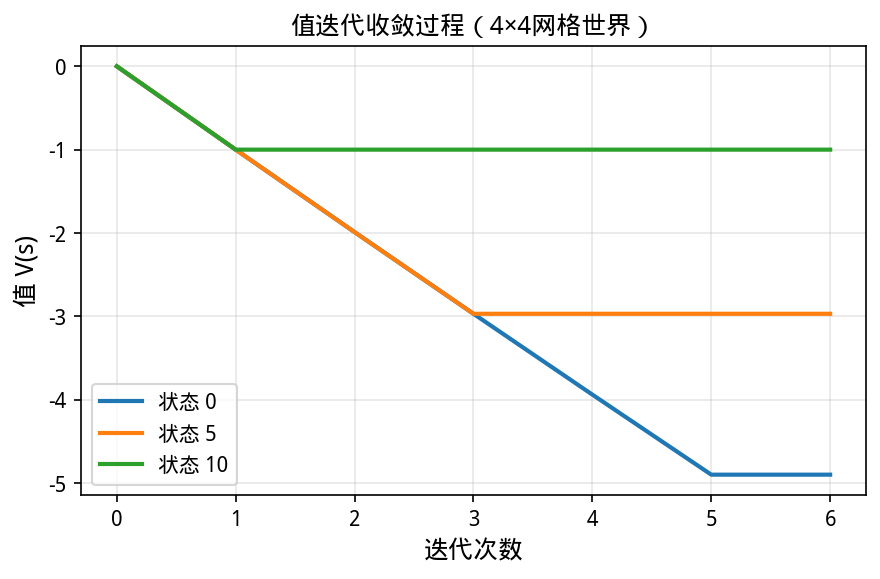
\includegraphics[width=\textwidth]{figs/chap10_value_iteration.png}
\end{minipage}
\hfill
\begin{minipage}{0.48\textwidth}
    \centering
    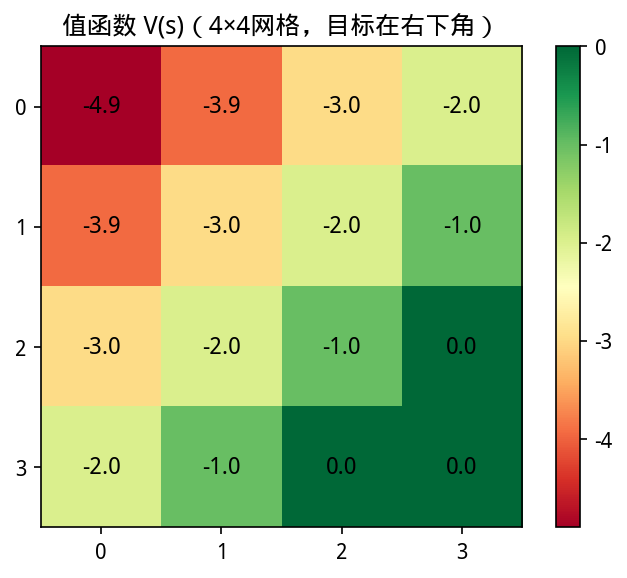
\includegraphics[width=\textwidth]{figs/chap10_value_heatmap.png}
\end{minipage}
\caption{值迭代结果。\textbf{左}：不同状态的值函数随迭代次数的变化，展示收敛过程；\textbf{右}：收敛后的值函数热力图，颜色越绿表示到达目标的期望回报越高。}
\label{fig:value_iteration}
\end{figure}

\begin{figure}[h]
\centering
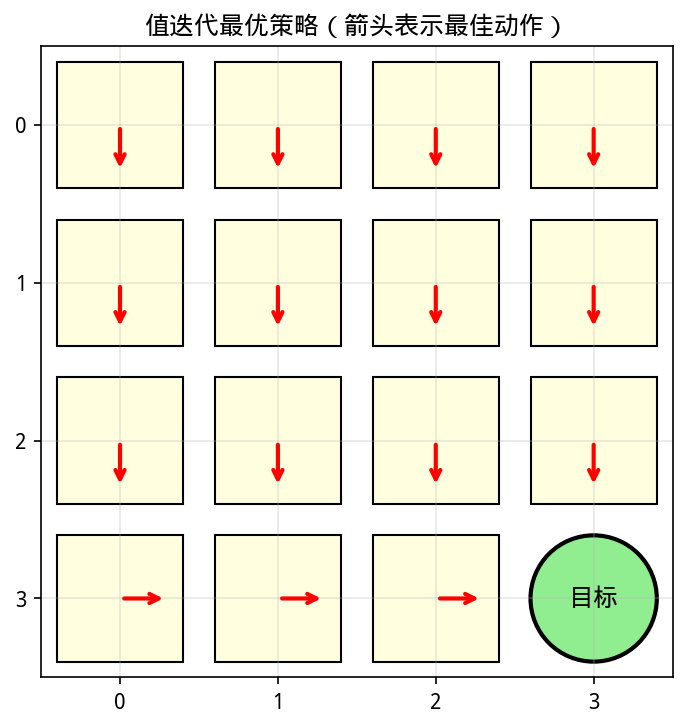
\includegraphics[width=0.45\textwidth]{figs/chap10_policy.png}
\caption{值迭代得到的最优策略。箭头指向每个状态应采取的最佳动作，指引智能体沿最短路径到达右下角的目标。}
\label{fig:policy}
\end{figure}

% ------------------------------------------------------------------------------------
\subsection{Q-Learning：从试错中学习}
% ------------------------------------------------------------------------------------

\marginnote{\textbf{Q-Learning的诞生}：Q-Learning由剑桥大学博士生Christopher Watkins在1989年博士论文中提出，1992年与Peter Dayan合作发表于\textit{Machine Learning}期刊。论文证明了Q-Learning在一定条件下收敛到最优Q函数，这个简洁的算法成为后来深度强化学习的基石。}

Q-Learning 是一种\textbf{无模型}方法。它不知道执行动作会发生什么，只能像小孩学走路一样——走一步、摔一跤、记住教训。

\begin{figure}[h]
\centering
\begin{tikzpicture}[scale=0.75]
    % 标题
    \node[font=\bfseries] at (2.5, 6.2) {Q-Learning：边走边学};
    
    % 画网格
    \draw[step=1, gray!50, thin] (0,0) grid (5,5);
    
    % 一条轨迹
    \fill[blue!20] (0,4) rectangle (1,5);
    \fill[blue!20] (1,4) rectangle (2,5);
    \fill[blue!20] (1,3) rectangle (2,4);
    \fill[blue!20] (2,3) rectangle (3,4);
    \fill[blue!20] (2,2) rectangle (3,3);
    
    % 轨迹箭头
    \draw[->, very thick, red!70] (0.5, 4.5) -- (1.3, 4.5);
    \draw[->, very thick, red!70] (1.5, 4.5) -- (1.5, 3.7);
    \draw[->, very thick, red!70] (1.5, 3.5) -- (2.3, 3.5);
    \draw[->, very thick, red!70] (2.5, 3.5) -- (2.5, 2.7);
    
    % 当前位置
    \node[circle, fill=red!70, minimum size=0.5cm] at (2.5, 2.5) {};
    
    % 终点
    \fill[green!30] (4,0) rectangle (5,1);
    
    % 说明
    \begin{scope}[xshift=6.5cm, yshift=2.5cm]
        \node[align=left, font=\small] at (0, 0) {
            每一步：\\[3pt]
            1. 选动作（探索/利用）\\
            2. 执行，观察 $s', r$\\
            3. 计算 TD 误差\\
            4. 更新 $Q(s,a)$\\
            5. 移动到 $s'$
        };
    \end{scope}
\end{tikzpicture}
\caption{Q-Learning 通过实际走动来学习。红色箭头表示智能体走过的轨迹，每走一步就更新一次 $Q$ 值。}
\end{figure}

\begin{lstlisting}[language=Python]
def q_learning(env, episodes=2000, gamma=1.0, alpha=0.1, epsilon=0.1):
    """
    Q-Learning 算法
    - 输入：环境 env（只能通过交互获取信息）
    - 输出：学到的 Q(s,a) 函数
    - 超参数：
        - episodes: 训练回合数
        - alpha: 学习率（每次更新的步长）
        - epsilon: 探索概率
    """
    Q = np.zeros((env.size, env.size, 4))  # Q(s, a) 初始化为 0
    
    for episode in range(episodes):
        state = (0, 0)  # 每个回合从起点开始
        
        # === 一个回合：从起点走到终点 ===
        while True:
            # --- 第一步：选择动作（epsilon-贪婪）---
            if np.random.random() < epsilon:
                action = np.random.randint(4)      # 10% 概率随机探索
            else:
                action = np.argmax(Q[state[0], state[1]])  # 90% 选当前最优；注意python张量特性
            
            # --- 第二步：执行动作，观察结果 ---
            # 注意：这是真实交互，不是模拟！
            next_state, reward, done = env.step(state, action)
            
            # --- 第三步：计算 TD 目标和误差 ---
            if done:
                td_target = reward  # 终点没有未来
            else:
                td_target = reward + gamma * np.max(Q[next_state])
            
            td_error = td_target - Q[state[0], state[1], action]
            
            # --- 第四步：更新 Q 值 ---
            # Q(s,a) ← Q(s,a) + α * (TD目标 - Q(s,a))
            Q[state[0], state[1], action] += alpha * td_error
            
            # --- 第五步：移动到下一状态 ---
            state = next_state
            if done:
                break  # 到达终点，结束本回合
    
    print(f"Q-Learning：训练了 {episodes} 个回合")
    return Q
\end{lstlisting}

\paragraph{算法要点}
\begin{itemize}
    \item \textbf{每个回合}：从起点走到终点，大约 8-20 步（取决于探索）
    \item \textbf{每一步}：只更新当前 $(s, a)$ 对应的 $Q$ 值（而不是所有状态）
    \item \textbf{探索 vs 利用}：$\epsilon = 0.1$ 意味着 10\% 概率随机探索，90\% 选当前最优
    \item \textbf{学习率}：$\alpha = 0.1$ 控制每次更新的幅度
    \item \textbf{计算量}：2000 回合 $\times$ 平均 10 步 $=$ 约 20000 次真实交互
\end{itemize}

\begin{figure}[h]
\centering
\begin{tikzpicture}[>=stealth]
    % TD 更新公式可视化
    \node[draw, rounded corners, fill=blue!10, minimum width=2.5cm, minimum height=1cm] (old) at (0, 0) {$Q(s,a)$};
    \node[draw, rounded corners, fill=green!10, minimum width=4cm, minimum height=1cm] (target) at (6, 0) {$r + \gamma \max_{a'} Q(s',a')$};
    \node[draw, rounded corners, fill=orange!10, minimum width=2.5cm, minimum height=1cm] (new) at (3, -2) {$Q(s,a)_{new}$};
    
    \draw[->, thick] (old) -- node[above] {TD 误差} (target);
    \draw[->, thick] (old) -- node[left] {$+ \alpha \cdot$} (new);
    \draw[->, thick] (target) -- node[right] {误差} (new);
    
    \node[below, font=\small, gray] at (3, -3) {$Q(s,a) \leftarrow Q(s,a) + \alpha \cdot \big[ \underbrace{r + \gamma \max_{a'} Q(s',a')}_{\text{TD 目标}} - Q(s,a) \big]$};
\end{tikzpicture}
\caption{Q-Learning 的更新规则：让 $Q(s,a)$ 向 TD 目标靠近一小步}
\end{figure}

% ------------------------------------------------------------------------------------
\subsection{对比：两种方法的本质区别}
% ------------------------------------------------------------------------------------

\begin{figure}[h]
\centering
\begin{tikzpicture}[scale=0.8, >=stealth]
    % 值迭代
    \begin{scope}[xshift=-5.5cm]
        \node[font=\bfseries] at (2, 4.5) {值迭代};
        \node[font=\small, gray] at (2, 4) {"在脑中推演"};
        
        \draw[step=0.6, gray!30, thin] (0,0) grid (3,3);
        
        % 遍历所有格子
        \foreach \i in {0,...,4} {
            \foreach \j in {0,...,4} {
                \fill[blue!30, opacity=0.5] (0.6*\i, 0.6*\j) rectangle (0.6*\i+0.6, 0.6*\j+0.6);
            }
        }
        
        \node[below, font=\small, align=center] at (1.5, -0.5) {每轮遍历\\所有状态};
    \end{scope}
    
    % Q-Learning
    \begin{scope}[xshift=2.5cm]
        \node[font=\bfseries] at (2, 4.5) {Q-Learning};
        \node[font=\small, gray] at (2, 4) {"边走边学"};
        
        \draw[step=0.6, gray!30, thin] (0,0) grid (3,3);
        
        % 只走过的格子
        \fill[red!30] (0, 2.4) rectangle (0.6, 3);
        \fill[red!30] (0.6, 2.4) rectangle (1.2, 3);
        \fill[red!30] (1.2, 2.4) rectangle (1.8, 3);
        \fill[red!30] (1.8, 1.8) rectangle (2.4, 2.4);
        \fill[red!30] (2.4, 1.2) rectangle (3, 1.8);
        \fill[red!30] (2.4, 0.6) rectangle (3, 1.2);
        \fill[red!30] (2.4, 0) rectangle (3, 0.6);
        
        % 轨迹线
        \draw[->, very thick, red!70] (0.3, 2.7) -- (0.9, 2.7) -- (1.5, 2.7) -- (2.1, 2.1) -- (2.7, 1.5) -- (2.7, 0.9) -- (2.7, 0.3);
        
        \node[below, font=\small, align=center] at (1.5, -0.5) {每回合只走\\一条轨迹};
    \end{scope}
\end{tikzpicture}
\caption{值迭代每轮更新所有状态；Q-Learning 每回合只更新走过的状态}
\end{figure}

运行两种算法，最终得到相同的值函数：
\newpage
\begin{verbatim}
=== 值迭代（需要模型）===
值迭代：9 轮后收敛

    [[-8. -7. -6. -5. -4.]
     [-7. -6. -5. -4. -3.]
     [-6. -5. -4. -3. -2.]
     [-5. -4. -3. -2. -1.]
     [-4. -3. -2. -1.  0.]]

=== Q-Learning（不需要模型）===
Q-Learning：训练了 2000 个回合

    [[-8. -7. -6. -5. -4.]
     [-7. -6. -5. -4. -3.]
     [-6. -5. -4. -3. -2.]
     [-5. -4. -3. -2. -1.]
     [-4. -3. -2. -1.  0.]]
\end{verbatim}

每个格子的最优价值 $=$ 到终点的曼哈顿距离的负值（因为每步 $-1$）。

\begin{table}[h]
\centering
\renewcommand{\arraystretch}{1.4}
\begin{tabular}{p{3cm}|p{5cm}|p{5cm}}
\toprule
& \textbf{值迭代} & \textbf{Q-Learning} \\
\midrule
\textbf{需要模型？} & 是（可以调用 \texttt{env.step} 模拟） & 否（只能真实交互） \\
\midrule
\textbf{每轮做什么} & 遍历所有 25 个状态 & 走一条轨迹（约 10 步） \\
\midrule
\textbf{收敛速度} & 9 轮（快！） & 2000 回合（慢） \\
\midrule
\textbf{计算量} & $9 \times 25 \times 4 = 900$ 次模型调用 & $\approx 20000$ 次真实交互 \\
\midrule
\textbf{适用场景} & 模型已知或可学习 & 模型未知或太复杂 \\
\bottomrule
\end{tabular}
\caption{值迭代 vs Q-Learning：速度与信息需求的权衡}
\end{table}

\begin{remark}
这个对比揭示了强化学习的核心权衡：
\begin{itemize}
    \item \textbf{有模型} $\Rightarrow$ 可以"想象"，数据效率高，但模型可能不准
    \item \textbf{无模型} $\Rightarrow$ 必须试错，数据效率低，但不怕模型偏差
\end{itemize}
在真实世界中，精确的环境模型往往难以获得，这就是为什么 Q-Learning 及其后继者（DQN、SAC 等）成为深度强化学习的主流方法。
\end{remark}

% ------------------------------------------------------------------------------------
% Q-Learning 实验结果
\begin{figure}[h]
\centering
\begin{minipage}{0.55\textwidth}
    \centering
    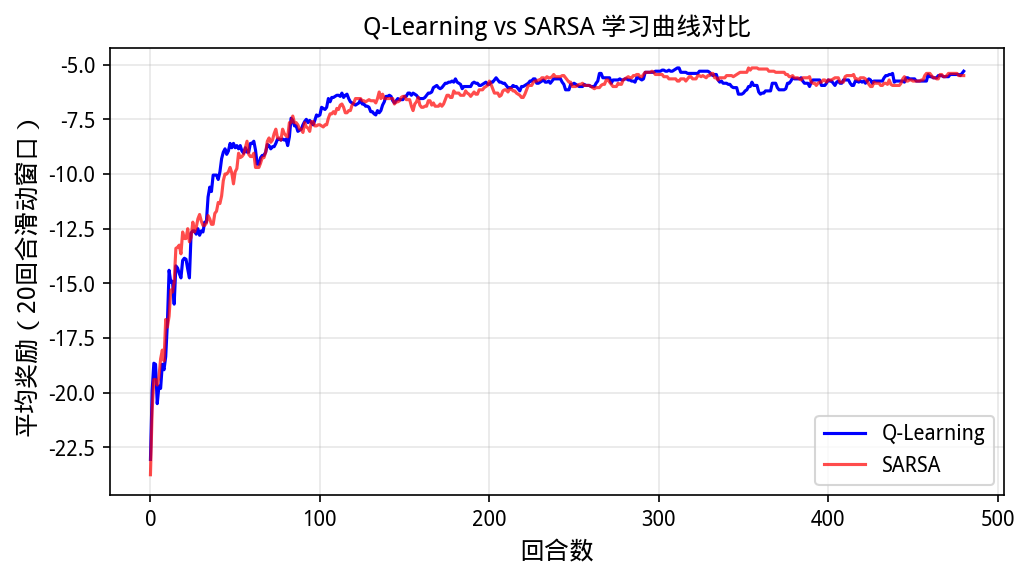
\includegraphics[width=\textwidth]{figs/chap10_qlearning_sarsa.png}
\end{minipage}
\hfill
\begin{minipage}{0.42\textwidth}
    \centering
    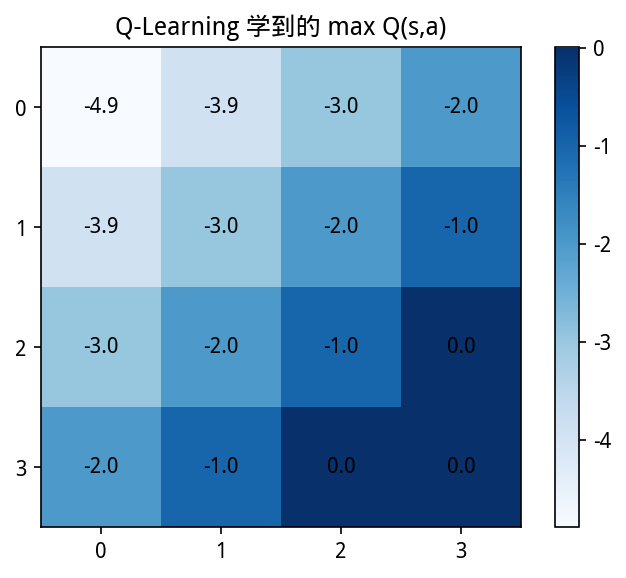
\includegraphics[width=\textwidth]{figs/chap10_qtable.png}
\end{minipage}
\caption{\textbf{左}：Q-Learning与SARSA的学习曲线对比。两种无模型算法通过与环境交互不断改进，最终都能学到接近最优的策略。\textbf{右}：Q-Learning学到的$\max_a Q(s,a)$热力图，可与图\ref{fig:value_iteration}中的值函数对比——虽然训练方式完全不同（无模型vs有模型），最终学到的值函数非常接近。}
\label{fig:qlearning_results}
\end{figure}

% ------------------------------------------------------------------------------------
\section{本章小结}
% ------------------------------------------------------------------------------------

让我们回顾这一章的核心内容：

\begin{enumerate}
    \item \textbf{贝尔曼方程的来源}：它不是凭空定义的，而是强化学习约束优化问题的KKT条件。值函数$V(s)$正是动力学约束的拉格朗日乘子。
    
    \item \textbf{最短路的启示}：通过最短路问题，我们看到了原始-对偶结构。Dijkstra代表"对偶上升"（维护最优性），Bellman-Ford代表"原始改进"（维护可行性）。
    
    \item \textbf{两个核心维度}：
    \begin{itemize}
        \item 模型可获取性：有模型（可以脑中模拟）vs 无模型（只能真实交互）
        \item 决策深度：浅（用估计值，低方差高偏差）vs 深（用真实回报，高方差低偏差）
    \end{itemize}
    
    \item \textbf{算法图谱}：动态规划、MCTS、蒙特卡洛、时序差分四大流派，以及它们的现代变体（PPO、GRPO等）。
\end{enumerate}

\begin{physicalmeaning}
强化学习的本质是：在\textbf{动力学约束}下，通过\textbf{试错与估计}找到最优决策。

不同算法的区别在于两个权衡：
\begin{itemize}
    \item 你知道多少规则？（模型）——决定能否"想象"而不必"实践"
    \item 你愿意看多远？（深度）——决定偏差与方差的取舍
\end{itemize}

从RLHF到GRPO，大语言模型对齐的最新进展告诉我们：当绝对的"奖励"难以定义时，"相对比较"（组内排序）是一条可行之路——这正是"原始改进"思想的现代演绎。
\end{physicalmeaning}

% ------------------------------------------------------------------------------------
\section{习题}
% ------------------------------------------------------------------------------------

\paragraph{概念理解}
\begin{enumerate}
    \item 用你自己的话解释：为什么说"值函数是拉格朗日乘子"？
    
    \item Dijkstra算法为什么不能处理负权边？用"对偶上升"的视角解释。
    
    \item TD学习的偏差来自哪里？在什么情况下这个偏差会特别严重？
    
    \item GRPO为什么不需要单独训练奖励模型？它和RLHF有什么本质区别？
\end{enumerate}

\paragraph{数学推导}
\begin{enumerate}
    \setcounter{enumi}{4}
    \item 写出最短路问题的原始LP和对偶LP，验证强对偶性成立。
    
    \item 证明：当$\gamma < 1$时，贝尔曼算子$T$是压缩映射，即
    \[
        \|TV_1 - TV_2\|_\infty \leq \gamma \|V_1 - V_2\|_\infty
    \]
    （提示：利用$|\max f - \max g| \leq \max |f - g|$）
\end{enumerate}

\paragraph{编程实践}
\begin{enumerate}
    \setcounter{enumi}{6}
    \item 修改GridWorld代码，添加一个"陷阱"格子（奖励$-10$）。观察值函数如何变化。
    
    \item 实现TD($\lambda$)算法，在GridWorld上比较$\lambda = 0, 0.5, 1$的学习曲线。
    
    \item （挑战）实现一个简化版的GRPO：对同一个状态采样多个动作，用组内排序来更新策略。
\end{enumerate}

\section{扩展阅读：从表格到神经网络}
% ------------------------------------------------------------------------------------

\marginnote{\textbf{Sutton与Barto}：Richard Sutton和Andrew Barto是强化学习领域的``教父''。他们1998年合著的《Reinforcement Learning: An Introduction》是该领域的圣经，免费在线阅读。Sutton提出了TD学习、策略梯度等核心算法，2024年获图灵奖提名。}

在前面的 GridWorld 例子中，我们用一个 $5 \times 5 \times 4$ 的数组来存储 $Q(s, a)$。这在状态空间很小的时候完全可行，但如果状态是一张 $84 \times 84$ 的游戏画面呢？

可能的状态数 $\approx 256^{84 \times 84} \approx 10^{17000}$

这个数字比宇宙中的原子数还要多得多。我们不可能为每个状态都存一个 $Q$ 值。

解决方案很自然：用\textbf{神经网络}来近似 $Q(s, a)$ 或 $\pi(a|s)$。这就是\textbf{深度强化学习}（Deep RL）的核心思想。

\begin{insightbox}
\textbf{为什么现代AI都围绕矩阵运算发展？}

你可能注意到了一个规律：从第3章的梯度计算，到第9章的反向传播，再到本章的强化学习，所有算法的核心都是\textbf{矩阵运算}。这不是巧合：

\begin{enumerate}
    \item \textbf{数学统一性}：神经网络的前向传播就是一系列矩阵乘法 $\bm{y} = \bm{W}\bm{x} + \bm{b}$；反向传播也是矩阵乘法的链式法则
    \item \textbf{硬件适配}：GPU 天生擅长并行矩阵运算，一块 A100 GPU 可以每秒完成 $10^{15}$ 次浮点矩阵运算
    \item \textbf{批量处理}：把 64 个样本打包成一个矩阵，一次前向传播就能处理所有样本
\end{enumerate}

所以，\textbf{理解矩阵运算 = 理解现代AI的计算基础}。这也是为什么我们在第2-3章花大量篇幅讲线性代数和矩阵求导。
\end{insightbox}

\begin{figure}[h]
\centering
\begin{tikzpicture}[>=stealth, scale=0.9]
    % 表格方法
    \begin{scope}[xshift=-5cm]
        \node[font=\bfseries] at (0, 3) {表格方法};
        
        % 表格
        \draw (0,0) grid[step=0.6] (1.8, 1.8);
        \foreach \i in {0,1,2} {
            \foreach \j in {0,1,2} {
                \node[font=\tiny] at (0.3+0.6*\i, 0.3+0.6*\j) {$Q$};
            }
        }
        
        \node[below, font=\small] at (0.9, -0.3) {每个格子存一个值};
        
        \draw[->, thick] (0, -1) -- (0, -1.8) node[below, font=\small, align=center] {状态数爆炸\\无法存储};
    \end{scope}
    
    % 箭头
    \draw[->, very thick] (-2, 1) -- (0, 1) node[midway, above, font=\small] {深度学习};
    
    % 神经网络方法
    \begin{scope}[xshift=3cm]
        \node[font=\bfseries] at (1.5, 3) {函数近似};
        
        % 输入
        \node[draw, rounded corners, fill=blue!20, minimum width=1.2cm, minimum height=1.5cm] (input) at (0, 1) {\small 状态 $s$};
        
        % 神经网络
        \node[draw, rounded corners, fill=orange!20, minimum width=1.5cm, minimum height=1.8cm, align=center] (nn) at (2.2, 1) {\small 神经\\网络};
        
        % 输出
        \node[draw, rounded corners, fill=green!20, minimum width=1.2cm, minimum height=1.5cm] (output) at (4.4, 1) {\small $Q(s,\cdot)$};
        
        \draw[->, thick] (input) -- (nn);
        \draw[->, thick] (nn) -- (output);
        
        \node[below, font=\small, align=center] at (2.2, -0.5) {网络参数 $\theta$\\可以泛化到未见过的状态};
    \end{scope}
\end{tikzpicture}
\caption{从表格方法到函数近似：神经网络用有限的参数表示无限状态空间上的值函数}
\end{figure}

% ------------------------------------------------------------------------------------
\subsection{Stable Baselines3：工业级深度强化学习库}
% ------------------------------------------------------------------------------------

\href{https://stable-baselines3.readthedocs.io/}{Stable Baselines3}（简称 SB3）是目前最流行的深度强化学习库。它实现了 DQN、PPO、SAC 等主流算法，代码清晰、文档完善，非常适合学习。

\begin{lstlisting}[language=Python, caption={用 SB3 训练一个 PPO 智能体}]
from stable_baselines3 import PPO
import gymnasium as gym

# 创建环境
env = gym.make("CartPole-v1")

# 创建智能体（一行代码！）
model = PPO("MlpPolicy", env, verbose=1)

# 训练
model.learn(total_timesteps=10000)

# 测试
obs, _ = env.reset()
for _ in range(1000):
    action, _ = model.predict(obs)
    obs, reward, done, _, _ = env.step(action)
    if done:
        obs, _ = env.reset()
\end{lstlisting}

看起来很简单，但背后隐藏着大量的工程细节。让我们深入源代码，看看这些算法到底是怎么实现的。

% ------------------------------------------------------------------------------------
\subsection{DQN：从 Q-Learning 到深度网络}
% ------------------------------------------------------------------------------------

\marginnote{\textbf{DeepMind与DQN}：2013年，伦敦创业公司DeepMind（由Demis Hassabis、Shane Legg等创立）在arXiv发布DQN论文，用神经网络玩Atari游戏达到人类水平。2014年Google以约6亿美元收购DeepMind。2015年DQN正式发表于Nature，开启深度强化学习时代。两年后AlphaGo击败世界围棋冠军，震惊世界。}

\marginnote{\textbf{Demis Hassabis}(1976--)：DeepMind联合创始人兼CEO，2024年诺贝尔化学奖得主（因AlphaFold蛋白质结构预测）。他是国际象棋神童，13岁时已是世界第二年轻的大师。他先后在剑桥和UCL获得学位，是少数同时在AI和神经科学两个领域做出重要贡献的人。}

DQN 是深度强化学习的开山之作（Mnih et al., 2015）。它的核心思想是用神经网络代替 Q 表格，但这带来了两个新问题：

\begin{enumerate}
    \item \textbf{数据相关性}：连续的游戏帧高度相关，直接训练会导致网络"过拟合"到最近的经验
    \item \textbf{目标不稳定}：TD 目标 $r + \gamma \max_{a'} Q(s', a')$ 依赖于 $Q$ 网络本身，形成"追逐移动靶心"
\end{enumerate}

DQN 的两个关键技巧正是为了解决这两个问题：

\begin{figure}[h]
\centering
\begin{tikzpicture}[>=stealth, scale=0.85]
    % 经验回放
    \begin{scope}[xshift=-4.5cm]
        \node[font=\bfseries] at (0, 3.5) {技巧一：经验回放};
        
        % 经验池
        \node[draw, rounded corners, fill=yellow!20, minimum width=3cm, minimum height=2cm] (buffer) at (0, 1.5) {};
        \node at (0, 2.2) {\small 经验池};
        
        % 经验条目
        \node[font=\tiny] at (0, 1.8) {$(s_1, a_1, r_1, s_1')$};
        \node[font=\tiny] at (0, 1.4) {$(s_2, a_2, r_2, s_2')$};
        \node[font=\tiny] at (0, 1.0) {$\vdots$};
        
        % 随机采样
        \draw[->, thick] (0, 0.3) -- (0, -0.5) node[below, font=\small, align=center] {随机采样\\打破相关性};
    \end{scope}
    
    % 目标网络
    \begin{scope}[xshift=3.5cm]
        \node[font=\bfseries] at (0, 3.5) {技巧二：目标网络};
        
        % 当前网络
        \node[draw, rounded corners, fill=blue!20, minimum width=2cm, minimum height=1cm] (q) at (-1.2, 2) {\small $Q_\theta$};
        \node[below, font=\tiny] at (-1.2, 1.4) {每步更新};
        
        % 目标网络
        \node[draw, rounded corners, fill=green!20, minimum width=2cm, minimum height=1cm] (qt) at (1.2, 2) {\small $Q_{\theta^-}$};
        \node[below, font=\tiny] at (1.2, 1.4) {定期复制};
        
        % 箭头
        \draw[->, thick, dashed] (q) -- node[above, font=\tiny] {周期性} (qt);
        
        % 说明
        \node[below, font=\small, align=center] at (0, 0) {用 $Q_{\theta^-}$ 计算目标\\稳定训练过程};
    \end{scope}
\end{tikzpicture}
\caption{DQN 的两个核心技巧}
\end{figure}

以下是 DQN 的核心训练逻辑（简化自 SB3 源码）。

\begin{insightbox}
\textbf{代码说明}：本节的 DQN、PPO、SAC 代码是\textbf{算法结构概览}，用于帮助理解核心逻辑。完整可运行的代码见 \texttt{code/chap10\_rl.py}（值迭代、Q-Learning、SARSA）和 Stable-Baselines3 库。

\textbf{为什么这里用概览代码？} 真实的 DQN/PPO 实现涉及大量工程细节（网络定义、数据加载、日志记录等），会淹没核心算法思想。我们先理解"骨架"，再去看完整实现。
\end{insightbox}

\begin{lstlisting}[language=Python, caption={DQN 核心算法（算法概览）}]
class DQN:
    def __init__(self, env):
        self.q_network = NeuralNetwork()        # Q 网络
        self.target_network = copy(self.q_network)  # 目标网络
        self.buffer = ReplayBuffer(size=100000)  # 经验池
        self.gamma = 0.99
        self.epsilon = 0.1  # 探索率
        
    def select_action(self, state):
        """epsilon-贪婪策略"""
        if random() < self.epsilon:
            return env.action_space.sample()  # 随机探索
        else:
            q_values = self.q_network(state)
            return argmax(q_values)  # 选最优
    
    def train_step(self, batch_size=64):
        """一步训练"""
        # 1. 从经验池随机采样
        states, actions, rewards, next_states, dones = \
            self.buffer.sample(batch_size)
        
        # 2. 计算 TD 目标（用目标网络！）
        with torch.no_grad():
            next_q_values = self.target_network(next_states)
            max_next_q = next_q_values.max(dim=1)
            td_target = rewards + self.gamma * max_next_q * (1 - dones)
        
        # 3. 计算当前 Q 值
        current_q = self.q_network(states)
        current_q = current_q.gather(1, actions)  # 选出执行动作的Q值
        
        # 4. 计算损失并更新（这就是 Bellman 误差！）
        loss = F.mse_loss(current_q, td_target)
        
        self.optimizer.zero_grad()
        loss.backward()
        self.optimizer.step()
        
    def update_target_network(self):
        """定期更新目标网络"""
        self.target_network.load_state_dict(
            self.q_network.state_dict()
        )
\end{lstlisting}

\begin{keyidea}[DQN 的损失函数就是 Bellman 误差]
\begin{equation}
    \mathcal{L}(\theta) = \mathbb{E}_{(s,a,r,s') \sim \mathcal{D}} \left[ \left( Q_\theta(s, a) - \underbrace{\left( r + \gamma \max_{a'} Q_{\theta^-}(s', a') \right)}_{\text{TD 目标（用目标网络）}} \right)^2 \right]
\end{equation}
这正是让 Bellman 方程"左边等于右边"的 L2 损失！
\end{keyidea}

% ------------------------------------------------------------------------------------
\subsection{PPO：稳健的策略梯度}
% ------------------------------------------------------------------------------------

\marginnote{\textbf{PPO与OpenAI}：PPO由OpenAI的John Schulman等人于2017年提出。Schulman此前还提出了TRPO（2015），但TRPO计算复杂。PPO通过简单的``裁剪''技巧获得类似效果，实现简单、调参容易，成为工业界标配。2022年ChatGPT的RLHF训练正是使用PPO，让AI学会遵循人类偏好。}

PPO（Proximal Policy Optimization）是目前工业界最常用的算法，ChatGPT 的 RLHF 训练就用的它。

与 DQN 不同，PPO 不是去拟合 Bellman 方程，而是\textbf{直接优化策略}。它的目标很直接：让好动作的概率变高，坏动作的概率变低。

\begin{figure}[h]
\centering
\begin{tikzpicture}[>=stealth, scale=0.9]
    % Actor-Critic 结构
    \node[draw, rounded corners, fill=blue!20, minimum width=2cm, minimum height=1.2cm] (state) at (0, 0) {状态 $s$};
    
    \node[draw, rounded corners, fill=orange!20, minimum width=2.5cm, minimum height=1.2cm] (actor) at (4, 1) {Actor $\pi_\theta$};
    \node[draw, rounded corners, fill=green!20, minimum width=2.5cm, minimum height=1.2cm] (critic) at (4, -1) {Critic $V_\phi$};
    
    \node[draw, rounded corners, fill=red!10, minimum width=2cm, minimum height=0.8cm] (action) at (8, 1) {动作 $a$};
    \node[draw, rounded corners, fill=purple!10, minimum width=2cm, minimum height=0.8cm] (value) at (8, -1) {价值 $V(s)$};
    
    \draw[->, thick] (state) -- (actor);
    \draw[->, thick] (state) -- (critic);
    \draw[->, thick] (actor) -- (action);
    \draw[->, thick] (critic) -- (value);
    
    \node[below, font=\small, gray] at (4, 1.8) {输出动作分布};
    \node[below, font=\small, gray] at (4, -0.2) {估计状态价值};
\end{tikzpicture}
\caption{PPO 的 Actor-Critic 结构：Actor 决定做什么，Critic 评估好不好}
\end{figure}

PPO 的核心创新是\textbf{Clip 机制}——限制每次更新的幅度，防止策略变化太大导致训练崩溃。

\begin{lstlisting}[language=Python, caption={PPO 核心算法}]
class PPO:
    def __init__(self, env):
        self.actor = PolicyNetwork()   # 策略网络 pi(a|s)
        self.critic = ValueNetwork()   # 价值网络 V(s)
        self.gamma = 0.99
        self.gae_lambda = 0.95  # GAE 参数
        self.clip_range = 0.2   # PPO 的核心：裁剪范围
        
    def collect_rollout(self, n_steps):
        """收集一段轨迹（On-policy：必须用当前策略！）"""
        trajectory = []
        state = self.env.reset()
        
        for _ in range(n_steps):
            with torch.no_grad():
                # Actor 输出动作分布，采样一个动作
                action_dist = self.actor(state)
                action = action_dist.sample()
                log_prob = action_dist.log_prob(action)
                value = self.critic(state)
            
            next_state, reward, done = self.env.step(action)
            trajectory.append({
                'state': state,
                'action': action,
                'log_prob': log_prob,  # 记住旧策略的概率
                'value': value,
                'reward': reward,
                'done': done
            })
            state = next_state
            
        return trajectory
    
    def compute_gae(self, trajectory):
        """计算广义优势估计（GAE）"""
        advantages = []
        gae = 0
        
        # 从后往前计算
        for t in reversed(range(len(trajectory))):
            if t == len(trajectory) - 1:
                next_value = 0
            else:
                next_value = trajectory[t+1]['value']
            
            # TD 误差
            delta = trajectory[t]['reward'] + \
                    self.gamma * next_value * (1 - trajectory[t]['done']) - \
                    trajectory[t]['value']
            
            # GAE 递推
            gae = delta + self.gamma * self.gae_lambda * gae
            advantages.insert(0, gae)
            
        return advantages
    
    def train(self, trajectory, advantages):
        """PPO 更新（可以用同一批数据更新多次！）"""
        
        # 计算回报（用于训练 Critic）
        returns = [adv + traj['value'] 
                   for adv, traj in zip(advantages, trajectory)]
        
        # 多个 epoch 更新（数据复用，但有 clip 保护）
        for epoch in range(K_EPOCHS):
            for batch in make_batches(trajectory):
                # --- Actor 损失：PPO-Clip ---
                
                # 新策略下的 log 概率
                new_dist = self.actor(batch['states'])
                new_log_prob = new_dist.log_prob(batch['actions'])
                
                # 概率比率 r(theta) = pi_new / pi_old
                ratio = torch.exp(new_log_prob - batch['old_log_probs'])
                
                # PPO 核心：裁剪目标
                surr1 = ratio * batch['advantages']
                surr2 = torch.clamp(ratio, 
                                    1 - self.clip_range,
                                    1 + self.clip_range) * batch['advantages']
                actor_loss = -torch.min(surr1, surr2).mean()
                
                # --- Critic 损失：简单的 MSE ---
                value_pred = self.critic(batch['states'])
                critic_loss = F.mse_loss(value_pred, batch['returns'])
                
                # --- 总损失 ---
                loss = actor_loss + 0.5 * critic_loss
                
                self.optimizer.zero_grad()
                loss.backward()
                self.optimizer.step()
        
        # On-policy：用完就丢！
        trajectory.clear()
\end{lstlisting}

\begin{keyidea}[PPO 的 Clip 机制]
\begin{equation}
    \mathcal{L}^{CLIP}(\theta) = \mathbb{E}_t \left[ \min \left( r_t(\theta) A_t, \; \text{clip}(r_t(\theta), 1-\epsilon, 1+\epsilon) A_t \right) \right]
\end{equation}
其中 $r_t(\theta) = \frac{\pi_\theta(a_t|s_t)}{\pi_{\theta_{old}}(a_t|s_t)}$ 是新旧策略的概率比。

当 $A_t > 0$（好动作）时，我们想增加 $r_t$，但最多增加到 $1+\epsilon$；\\
当 $A_t < 0$（坏动作）时，我们想减少 $r_t$，但最多减少到 $1-\epsilon$。

这样就防止了策略更新"步子迈太大"。
\end{keyidea}

% ------------------------------------------------------------------------------------
\subsection{SAC：最大熵强化学习}
% ------------------------------------------------------------------------------------

\marginnote{\textbf{SAC与Berkeley}：SAC由UC Berkeley的Tuomas Haarnoja等人于2018年提出，导师是Pieter Abbeel和Sergey Levine——两位机器人强化学习的领军人物。SAC的``最大熵''思想来自信息论，让策略保持适度随机性以增强探索和鲁棒性，在机器人操作任务中表现出色。}

SAC（Soft Actor-Critic）是连续控制任务的首选算法，在机器人控制领域表现优异。

SAC 的核心思想是：不仅要最大化奖励，还要最大化策略的\textbf{熵}（随机性）。这听起来很奇怪——我们不是应该找到最优动作然后一直执行吗？

\begin{figure}[h]
\centering
\begin{tikzpicture}[>=stealth, scale=0.9]
    % 普通 RL
    \begin{scope}[xshift=-4cm]
        \node[font=\bfseries] at (0, 3.5) {普通 RL};
        
        \draw[->] (-1.5, 0) -- (1.5, 0) node[right] {$a$};
        \draw[->] (0, 0) -- (0, 2) node[above] {$\pi(a|s)$};
        
        % 尖峰分布
        \draw[thick, blue, fill=blue!20] (-0.1, 0) -- (0, 1.8) -- (0.1, 0) -- cycle;
        
        \node[below, font=\small] at (0, -0.5) {确定性策略};
        \node[below, font=\tiny, gray] at (0, -1) {容易陷入局部最优};
    \end{scope}
    
    % SAC
    \begin{scope}[xshift=4cm]
        \node[font=\bfseries] at (0, 3.5) {SAC（最大熵）};
        
        \draw[->] (-1.5, 0) -- (1.5, 0) node[right] {$a$};
        \draw[->] (0, 0) -- (0, 2) node[above] {$\pi(a|s)$};
        
        % 高斯分布
        \draw[thick, red, fill=red!20, domain=-1.3:1.3, samples=50] 
            plot (\x, {1.5*exp(-2*\x*\x)});
        
        \node[below, font=\small] at (0, -0.5) {随机策略};
        \node[below, font=\tiny, gray] at (0, -1) {保持探索，更鲁棒};
    \end{scope}
\end{tikzpicture}
\caption{普通 RL 学出尖锐的确定性策略，SAC 保持策略的随机性}
\end{figure}

为什么要保持随机性？
\begin{itemize}
    \item \textbf{更好的探索}：随机策略能发现更多可能性
    \item \textbf{更强的鲁棒性}：面对扰动时不会彻底崩溃
    \item \textbf{避免局部最优}：不会过早锁死在某个策略上
\end{itemize}

\begin{lstlisting}[language=Python, caption={SAC 核心算法}]
class SAC:
    def __init__(self, env):
        # SAC 有 5 个网络！
        self.actor = GaussianPolicy()     # 输出动作的均值和方差
        self.critic_1 = QNetwork()        # Q1(s, a)
        self.critic_2 = QNetwork()        # Q2(s, a) - 双Q减少过估计
        self.target_critic_1 = copy(self.critic_1)
        self.target_critic_2 = copy(self.critic_2)
        
        self.alpha = 0.2  # 熵系数（温度）
        self.buffer = ReplayBuffer()
        
    def select_action(self, state):
        """从高斯分布采样动作"""
        mean, std = self.actor(state)
        dist = Normal(mean, std)
        action = dist.rsample()  # 重参数化采样（可导！）
        return torch.tanh(action)  # 压缩到 [-1, 1]
    
    def train_step(self, batch_size=256):
        batch = self.buffer.sample(batch_size)
        
        # --- 更新 Critic ---
        with torch.no_grad():
            # 用当前策略采样下一个动作
            next_action, next_log_prob = self.actor.sample(
                batch['next_states']
            )
            
            # 双Q网络：取较小的那个（悲观估计）
            target_q1 = self.target_critic_1(
                batch['next_states'], next_action
            )
            target_q2 = self.target_critic_2(
                batch['next_states'], next_action
            )
            target_q = torch.min(target_q1, target_q2)
            
            # SAC 的目标：Q - alpha * log_prob（软Q值）
            target = batch['rewards'] + self.gamma * (
                target_q - self.alpha * next_log_prob
            )
        
        # Critic 损失
        q1 = self.critic_1(batch['states'], batch['actions'])
        q2 = self.critic_2(batch['states'], batch['actions'])
        critic_loss = F.mse_loss(q1, target) + F.mse_loss(q2, target)
        
        self.critic_optimizer.zero_grad()
        critic_loss.backward()
        self.critic_optimizer.step()
        
        # --- 更新 Actor ---
        # 重参数化技巧：a = tanh(mu + sigma * epsilon)
        new_action, log_prob = self.actor.rsample(batch['states'])
        
        q_value = torch.min(
            self.critic_1(batch['states'], new_action),
            self.critic_2(batch['states'], new_action)
        )
        
        # Actor 目标：最大化 Q - alpha * log_prob
        # 等价于最小化 alpha * log_prob - Q
        actor_loss = (self.alpha * log_prob - q_value).mean()
        
        self.actor_optimizer.zero_grad()
        actor_loss.backward()
        self.actor_optimizer.step()
        
        # --- 软更新目标网络（Polyak 平均）---
        for target_param, param in zip(
            self.target_critic_1.parameters(),
            self.critic_1.parameters()
        ):
            target_param.data.copy_(
                0.995 * target_param.data + 0.005 * param.data
            )
        # target_critic_2 同理
\end{lstlisting}

\begin{keyidea}[title=SAC 的优化目标]
SAC 最大化的不是普通的累积奖励，而是带熵正则的目标：
\begin{equation}
    J(\pi) = \sum_{t=0}^{\infty} \mathbb{E}_{(s_t, a_t) \sim \pi} \left[ r(s_t, a_t) + \alpha \underbrace{\mathcal{H}(\pi(\cdot|s_t))}_{\text{策略熵}} \right]
\end{equation}
其中 $\alpha$ 是温度系数，控制"探索 vs 利用"的权衡。
\end{keyidea}

% ------------------------------------------------------------------------------------
\subsection{三种算法的对比总结}
% ------------------------------------------------------------------------------------

\begin{table}[h]
\centering
\small
\renewcommand{\arraystretch}{1.4}
\caption{DQN、PPO、SAC 的核心对比}
\begin{tabular}{p{2.2cm}|p{3.8cm}|p{3.8cm}|p{3.8cm}}
\toprule
& \textbf{DQN} & \textbf{PPO} & \textbf{SAC} \\
\midrule
\textbf{学什么} & Q 值函数 $Q(s,a)$ & 策略 $\pi(a|s)$ + 价值 $V(s)$ & 策略 $\pi(a|s)$ + Q值 $Q(s,a)$ \\
\midrule
\textbf{动作空间} & 离散 & 离散或连续 & 连续 \\
\midrule
\textbf{数据策略} & Off-policy（经验回放） & On-policy（用完即弃） & Off-policy（经验回放） \\
\midrule
\textbf{核心技巧} & 目标网络 & Clip 裁剪 & 最大熵 + 双Q网络 \\
\midrule
\textbf{损失函数} & Bellman 误差 (MSE) & Clip 策略损失 + 价值 MSE & 软 Bellman 误差 + 策略熵 \\
\midrule
\textbf{典型应用} & Atari 游戏 & ChatGPT、机器人 & 机器人控制 \\
\bottomrule
\end{tabular}
\end{table}

\begin{figure}[h]
\centering
\begin{tikzpicture}[scale=0.9]
    % 坐标轴
    \draw[->, thick] (-0.5, 0) -- (10, 0) node[right] {实现复杂度};
    \draw[->, thick] (0, -0.5) -- (0, 5) node[above] {样本效率};
    
    % 算法位置
    \node[draw, circle, fill=blue!30, minimum size=1.2cm] (dqn) at (2, 2) {DQN};
    \node[draw, circle, fill=orange!30, minimum size=1.2cm] (ppo) at (5, 3) {PPO};
    \node[draw, circle, fill=green!30, minimum size=1.2cm] (sac) at (8, 4.5) {SAC};
    
    % 标注
    \node[below, font=\small] at (2, 1.2) {简单、入门};
    \node[below, font=\small] at (5, 2.2) {稳健、通用};
    \node[below, font=\small] at (8, 3.7) {高效、复杂};
    
    % 箭头表示演进
    \draw[->, dashed, gray] (dqn) -- (ppo);
    \draw[->, dashed, gray] (ppo) -- (sac);
\end{tikzpicture}
\caption{三种算法的定位：从简单到复杂，从低效到高效}
\end{figure}

% ------------------------------------------------------------------------------------
\subsection{动手实践：用 SB3 训练经典控制任务}
% ------------------------------------------------------------------------------------

以下代码展示如何用 SB3 在经典控制任务上训练和对比三种算法：

\begin{lstlisting}[language=Python, caption={用 SB3 对比三种算法}]
import gymnasium as gym
from stable_baselines3 import DQN, PPO, SAC
import matplotlib.pyplot as plt

# CartPole: 离散动作，适合 DQN 和 PPO
env_discrete = gym.make("CartPole-v1")

# Pendulum: 连续动作，适合 PPO 和 SAC
env_continuous = gym.make("Pendulum-v1")

# --- 训练 DQN（离散动作）---
dqn_model = DQN(
    "MlpPolicy", 
    env_discrete,
    learning_rate=1e-3,
    buffer_size=50000,      # 经验池大小
    learning_starts=1000,   # 开始训练前先收集多少数据
    target_update_interval=500,  # 目标网络更新频率
    verbose=1
)
dqn_model.learn(total_timesteps=20000)

# --- 训练 PPO（通用）---
ppo_model = PPO(
    "MlpPolicy",
    env_discrete,
    learning_rate=3e-4,
    n_steps=2048,           # 每次收集多少步
    batch_size=64,          # 小批量大小
    n_epochs=10,            # 每批数据训练几轮
    clip_range=0.2,         # PPO clip 参数
    verbose=1
)
ppo_model.learn(total_timesteps=20000)

# --- 训练 SAC（连续动作）---
sac_model = SAC(
    "MlpPolicy",
    env_continuous,
    learning_rate=3e-4,
    buffer_size=100000,
    learning_starts=1000,
    tau=0.005,              # 软更新系数
    verbose=1
)
sac_model.learn(total_timesteps=20000)
\end{lstlisting}

\begin{remark}
SB3 的强大之处在于：\textbf{把这里的 \texttt{CartPole} 换成你的自定义环境，代码几乎不用改}。

只要你的问题能封装成 Gymnasium 接口：
\begin{itemize}
    \item \texttt{reset()} 返回初始状态
    \item \texttt{step(action)} 返回 (下一状态, 奖励, 是否结束, 信息)
\end{itemize}

那么 SB3 就能直接训练。把 CartPole 的物理方程换成飞行器动力学，就是飞行控制；换成流体方程，就是流体控制。
\end{remark}




\section{扩展阅读：深度强化学习与约束优化的深层联系}
% ------------------------------------------------------------------------------------

在第一章中，我们用拉格朗日乘子法推导出了贝尔曼方程。现在让我们反过来思考：既然强化学习本质上是一个约束优化问题，那么现代算法（如 PPO）是如何处理这些约束的？

这一节我们将揭示 PPO 背后的优化理论，以及从 TRPO 到 PPO 的演化过程中，研究者是如何用工程技巧来近似复杂的约束优化的。

% ------------------------------------------------------------------------------------
\subsection{策略优化的本质困难}
% ------------------------------------------------------------------------------------

假设我们想直接优化策略 $\pi_\theta$，最大化累积奖励：
\begin{equation}
    \max_\theta \; J(\theta) = \mathbb{E}_{\tau \sim \pi_\theta} \left[ \sum_{t=0}^{T} \gamma^t r_t \right]
\end{equation}

这看起来就是一个普通的优化问题，用梯度上升不就行了吗？

\begin{equation}
    \theta \leftarrow \theta + \alpha \nabla_\theta J(\theta)
\end{equation}

问题在于：\textbf{策略梯度的方差极大，而且步长很难选择}。

\begin{figure}[h]
\centering
\begin{tikzpicture}[>=stealth, scale=0.9]
    % 损失曲面
    \draw[thick, domain=-3:3, samples=100, blue] 
        plot (\x, {0.3*\x*\x - 0.5*cos(3*\x r) + 2});
    
    % 当前位置
    \fill[red] (-1.5, 2.175) circle (3pt);
    \node[above right, font=\small] at (-1.5, 2.175) {当前策略 $\theta$};
    
    % 小步长
    \draw[->, thick, green!60!black] (-1.5, 2.175) -- (-0.8, 1.8);
    \node[below, font=\scriptsize, green!60!black] at (-1.15, 1.8) {小步长：安全但慢};
    
    % 大步长（跳过去）
    \draw[->, thick, red, dashed] (-1.5, 2.175) -- (1.5, 2.5);
    \node[above, font=\scriptsize, red] at (0, 2.8) {大步长：可能跳到很差的地方};
    
    % 悬崖
    \fill[red!20] (0.8, 0) rectangle (1.2, 3.5);
    \node[font=\scriptsize, red] at (1, 3.8) {性能悬崖};
    
    \draw[->] (-3.5, 0) -- (3.5, 0) node[right] {$\theta$};
    \draw[->] (-3, -0.5) -- (-3, 4) node[above] {$-J(\theta)$};
\end{tikzpicture}
\caption{策略优化的困难：损失曲面高度非凸，步长太大可能跳入"性能悬崖"}
\end{figure}

更糟糕的是，策略的微小变化可能导致\textbf{采样分布的巨大变化}。想象一下：

\begin{itemize}
    \item 旧策略 $\pi_{old}$：在状态 $s$ 有 90\% 概率选动作 $a_1$
    \item 新策略 $\pi_{new}$：在状态 $s$ 有 90\% 概率选动作 $a_2$
\end{itemize}

虽然参数 $\theta$ 可能只变了一点点，但智能体的行为完全不同了！这就是为什么普通的梯度下降在策略优化中经常失败。

% ------------------------------------------------------------------------------------
\subsection{信任域方法：把优化问题变成约束优化}
% ------------------------------------------------------------------------------------

解决方案是：\textbf{限制每次更新的幅度}。

这正是\textbf{信任域方法}（Trust Region Methods）的核心思想。我们不是在整个参数空间里找最优，而是在当前点附近的一个"信任域"里找最优。

\begin{keyidea}[信任域优化]
每一步解决以下约束优化问题：
\begin{equation}
    \begin{aligned}
        \max_\theta \quad & L(\theta) = \mathbb{E}_{s,a \sim \pi_{old}} \left[ \frac{\pi_\theta(a|s)}{\pi_{old}(a|s)} A^{\pi_{old}}(s,a) \right] \\
        \text{s.t.} \quad & D(\pi_\theta, \pi_{old}) \leq \delta
    \end{aligned}
\end{equation}
其中 $D$ 是某种"距离"度量，$\delta$ 是信任域半径。
\end{keyidea}

这里的 $L(\theta)$ 叫做\textbf{替代目标}（Surrogate Objective）。它的含义是：

\begin{itemize}
    \item $\frac{\pi_\theta(a|s)}{\pi_{old}(a|s)}$：新旧策略的概率比
    \item $A^{\pi_{old}}(s,a)$：在旧策略下，动作 $a$ 比平均水平好多少（优势函数）
    \item 整体意义：如果 $A > 0$（好动作），增大概率比；如果 $A < 0$（坏动作），减小概率比
\end{itemize}

% ------------------------------------------------------------------------------------
\subsection{TRPO：用拉格朗日对偶求解}
% ------------------------------------------------------------------------------------

TRPO（Trust Region Policy Optimization）选择 KL 散度作为距离度量：

\begin{equation}
    \begin{aligned}
        \max_\theta \quad & L(\theta) \\
        \text{s.t.} \quad & \bar{D}_{KL}(\pi_{old} \| \pi_\theta) \leq \delta
    \end{aligned}
\end{equation}

其中 $\bar{D}_{KL}$ 是对所有状态取平均的 KL 散度。

\paragraph{拉格朗日对偶}

这是一个不等式约束优化问题，自然想到用拉格朗日乘子法：

\begin{equation}
    \mathcal{L}(\theta, \lambda) = L(\theta) - \lambda \left( \bar{D}_{KL}(\pi_{old} \| \pi_\theta) - \delta \right)
\end{equation}

对偶问题是：
\begin{equation}
    \min_{\lambda \geq 0} \max_\theta \mathcal{L}(\theta, \lambda)
\end{equation}

\paragraph{二阶近似与自然梯度}

TRPO 的关键洞察是：在 $\theta_{old}$ 附近，可以用泰勒展开近似：

\begin{align}
    L(\theta) &\approx L(\theta_{old}) + g^T (\theta - \theta_{old}) \\
    \bar{D}_{KL} &\approx \frac{1}{2} (\theta - \theta_{old})^T F (\theta - \theta_{old})
\end{align}

其中 $g = \nabla_\theta L|_{\theta_{old}}$ 是策略梯度，$F$ 是\textbf{Fisher 信息矩阵}：

\begin{equation}
    F = \mathbb{E}_{s \sim \pi_{old}} \left[ \nabla_\theta \log \pi_\theta(a|s) \nabla_\theta \log \pi_\theta(a|s)^T \right]_{\theta = \theta_{old}}
\end{equation}

这样，约束优化问题变成了一个\textbf{二次规划}：

\begin{equation}
    \begin{aligned}
        \max_{\Delta\theta} \quad & g^T \Delta\theta \\
        \text{s.t.} \quad & \frac{1}{2} \Delta\theta^T F \Delta\theta \leq \delta
    \end{aligned}
\end{equation}

用 KKT 条件可以得到解析解：

\begin{equation}
    \Delta\theta^* = \sqrt{\frac{2\delta}{g^T F^{-1} g}} F^{-1} g
\end{equation}

这就是\textbf{自然梯度}（Natural Gradient）！它的方向是 $F^{-1} g$，不是普通梯度 $g$。

\begin{figure}[h]
\centering
\begin{tikzpicture}[>=stealth, scale=1.0]
    % 椭圆等高线（KL 约束）
    \draw[thick, blue, rotate=30] (0,0) ellipse (2 and 1);
    \draw[thick, blue!60, rotate=30] (0,0) ellipse (1.5 and 0.75);
    \draw[thick, blue!30, rotate=30] (0,0) ellipse (1 and 0.5);
    
    % 当前点
    \fill[red] (0, 0) circle (3pt);
    \node[below left, font=\small] at (0, 0) {$\theta_{old}$};
    
    % 普通梯度方向
    \draw[->, very thick, green!60!black] (0, 0) -- (1.5, 0.8);
    \node[right, font=\small, green!60!black] at (1.5, 0.8) {普通梯度 $g$};
    
    % 自然梯度方向
    \draw[->, very thick, red] (0, 0) -- (1.2, -0.3);
    \node[right, font=\small, red] at (1.2, -0.3) {自然梯度 $F^{-1}g$};
    
    % 信任域边界
    \node[blue, font=\small] at (2.2, 1.5) {KL $= \delta$};
    
    % 说明
    \node[below, font=\small, align=center] at (0, -2) {自然梯度考虑了参数空间的"形状"\\在 KL 约束下是最优方向};
\end{tikzpicture}
\caption{普通梯度 vs 自然梯度。椭圆是 KL 散度的等高线，自然梯度是在 KL 约束下的最优方向。}
\end{figure}

\paragraph{TRPO 的数值困难}

TRPO 理论很漂亮，但实现很困难：

\begin{enumerate}
    \item \textbf{Fisher 矩阵太大}：如果网络有 $n$ 个参数，$F$ 是 $n \times n$ 矩阵。对于百万参数的网络，存储和求逆都不可行。
    
    \item \textbf{需要共轭梯度法}：TRPO 用共轭梯度（CG）来近似求解 $F^{-1}g$，需要多次计算 $Fv$（Fisher-向量乘积）。
    
    \item \textbf{需要线搜索}：二阶近似可能不准，TRPO 还需要做线搜索来确保约束真的满足。
\end{enumerate}

\begin{lstlisting}[language=Python, caption={TRPO 的核心步骤（简化版）}]
def trpo_update(policy, states, actions, advantages):
    # 1. 计算策略梯度
    g = compute_policy_gradient(policy, states, actions, advantages)
    
    # 2. 用共轭梯度法求解 F^{-1} g
    def fisher_vector_product(v):
        # 计算 Fv，不需要显式构造 F
        return compute_fvp(policy, states, v)
    
    step_dir = conjugate_gradient(fisher_vector_product, g, max_iter=10)
    
    # 3. 计算步长
    shs = 0.5 * step_dir.dot(fisher_vector_product(step_dir))
    step_size = sqrt(2 * delta / shs)
    full_step = step_size * step_dir
    
    # 4. 线搜索：确保 KL 约束满足且目标提升
    for shrink in [1, 0.5, 0.25, 0.125]:
        new_params = old_params + shrink * full_step
        if kl_divergence(new_policy, old_policy) <= delta:
            if surrogate_loss(new_policy) > surrogate_loss(old_policy):
                break
    
    return new_params
\end{lstlisting}

% ------------------------------------------------------------------------------------
\subsection{PPO：用裁剪代替约束}
% ------------------------------------------------------------------------------------

PPO 的核心洞察是：\textbf{与其精确求解约束优化，不如用一个简单的裁剪来近似}。

回顾 TRPO 的目标：
\begin{equation}
    \max_\theta \; \mathbb{E} \left[ \frac{\pi_\theta(a|s)}{\pi_{old}(a|s)} A(s,a) \right] \quad \text{s.t.} \quad D_{KL} \leq \delta
\end{equation}

PPO 的想法是：与其用 KL 散度约束概率比 $r(\theta) = \frac{\pi_\theta}{\pi_{old}}$，不如\textbf{直接裁剪概率比}！

\begin{keyidea}[PPO-Clip 目标函数]
\begin{equation}
    L^{CLIP}(\theta) = \mathbb{E} \left[ \min \left( r(\theta) A, \; \text{clip}(r(\theta), 1-\epsilon, 1+\epsilon) A \right) \right]
\end{equation}
其中 $\epsilon$ 通常取 $0.1$ 或 $0.2$。
\end{keyidea}

让我们仔细理解这个公式：

\begin{figure}[h]
\centering
\begin{tikzpicture}[>=stealth, scale=0.85]
    % A > 0 的情况
    \begin{scope}[xshift=-5cm]
        \node[font=\bfseries] at (2, 4) {当 $A > 0$（好动作）};
        
        \draw[->] (0, 0) -- (4.5, 0) node[right] {$r(\theta)$};
        \draw[->] (0, -0.5) -- (0, 3.5) node[above] {目标};
        
        % 未裁剪的目标
        \draw[thick, blue, dashed] (0, 0) -- (4, 3.2);
        \node[blue, font=\scriptsize] at (3.8, 2.5) {$rA$};
        
        % 裁剪后的目标
        \draw[very thick, red] (0, 0) -- (2.4, 1.92);
        \draw[very thick, red] (2.4, 1.92) -- (4, 1.92);
        
        % 裁剪点
        \draw[dashed, gray] (2.4, 0) -- (2.4, 1.92);
        \node[below, font=\scriptsize] at (2.4, 0) {$1+\epsilon$};
        \node[below, font=\scriptsize] at (1, 0) {$1$};
        \draw[dashed, gray] (1, 0) -- (1, 0.8);
        
        \node[below, font=\small, align=center] at (2, -1) {概率比超过 $1+\epsilon$ 后\\目标不再增加};
    \end{scope}
    
    % A < 0 的情况
    \begin{scope}[xshift=4cm]
        \node[font=\bfseries] at (2, 4) {当 $A < 0$（坏动作）};
        
        \draw[->] (0, 0) -- (4.5, 0) node[right] {$r(\theta)$};
        \draw[->] (0, -2.5) -- (0, 1) node[above] {目标};
        
        % 未裁剪的目标
        \draw[thick, blue, dashed] (0, 0) -- (4, -3.2);
        \node[blue, font=\scriptsize] at (3.8, -2.5) {$rA$};
        
        % 裁剪后的目标
        \draw[very thick, red] (0, 0) -- (0.8, -0.64);
        \draw[very thick, red] (0.8, -0.64) -- (4, -0.64);
        
        % 裁剪点
        \draw[dashed, gray] (0.8, 0) -- (0.8, -0.64);
        \node[below, font=\scriptsize] at (0.8, 0) {$1-\epsilon$};
        \node[below, font=\scriptsize] at (2, 0) {$1$};
        \draw[dashed, gray] (2, 0) -- (2, -0.5);
        
        \node[below, font=\small, align=center] at (2, -3.5) {概率比低于 $1-\epsilon$ 后\\目标不再减少};
    \end{scope}
\end{tikzpicture}
\caption{PPO 裁剪机制的效果。左：对于好动作，限制概率增加的幅度。右：对于坏动作，限制概率减少的幅度。}
\end{figure}

\paragraph{为什么裁剪有效？}

\begin{itemize}
    \item 当 $A > 0$（好动作）：我们想增大 $r(\theta)$，但超过 $1+\epsilon$ 后梯度消失，防止过度增加
    \item 当 $A < 0$（坏动作）：我们想减小 $r(\theta)$，但低于 $1-\epsilon$ 后梯度消失，防止过度减少
\end{itemize}

这相当于\textbf{隐式地}限制了策略的变化幅度，而不需要显式计算 KL 散度或 Fisher 矩阵！

\paragraph{PPO vs TRPO 的数值比较}

\begin{table}[h]
\centering
\renewcommand{\arraystretch}{1.4}
\begin{tabular}{p{3cm}|p{5cm}|p{5cm}}
\toprule
& \textbf{TRPO} & \textbf{PPO} \\
\midrule
\textbf{约束方式} & 显式 KL 散度约束 & 隐式裁剪 \\
\midrule
\textbf{需要计算} & Fisher 矩阵、共轭梯度、线搜索 & 只需要普通梯度 \\
\midrule
\textbf{每次更新} & 一步精确求解 & 多个 epoch 小步迭代 \\
\midrule
\textbf{实现难度} & 高（约 500 行核心代码） & 低（约 50 行核心代码） \\
\midrule
\textbf{计算成本} & 高（每步需要多次前向/反向传播） & 低（标准梯度下降） \\
\midrule
\textbf{性能} & 理论最优 & 实践中相当甚至更好 \\
\bottomrule
\end{tabular}
\caption{TRPO vs PPO：复杂度与性能的权衡}
\end{table}

% ------------------------------------------------------------------------------------
\subsection{PPO 的完整优化流程}
% ------------------------------------------------------------------------------------

让我们详细看看 PPO 的一次完整更新：

\begin{figure}[h]
\centering
\begin{tikzpicture}[>=stealth, scale=0.85, 
    block/.style={draw, rounded corners, minimum width=2.5cm, minimum height=1cm, align=center}]
    
    % 流程图
    \node[block, fill=blue!20] (collect) at (0, 0) {收集轨迹\\$\{s, a, r, \log\pi_{old}\}$};
    \node[block, fill=green!20] (gae) at (5, 0) {计算优势\\GAE};
    \node[block, fill=orange!20] (epoch) at (10, 0) {多轮训练\\K epochs};
    \node[block, fill=red!20] (discard) at (10, -2.5) {丢弃数据\\(On-policy)};
    
    \draw[->, thick] (collect) -- (gae);
    \draw[->, thick] (gae) -- (epoch);
    \draw[->, thick] (epoch) -- (discard);
    \draw[->, thick, dashed] (discard) -- (0, -2.5) -- (collect);
    
    % epoch 内部
    \begin{scope}[xshift=10cm, yshift=-5.5cm]
        \node[font=\bfseries] at (-5, 2.5) {每个 Epoch 内部};
        
        \node[block, fill=yellow!20, minimum width=2cm] (batch) at (0, 1.5) {采样 batch};
        \node[block, fill=purple!20, minimum width=2cm] (ratio) at (0, 0) {计算 $r(\theta)$};
        \node[block, fill=cyan!20, minimum width=2cm] (clip) at (0, -1.5) {裁剪 + 损失};
        \node[block, fill=gray!20, minimum width=2cm] (grad) at (0, -3) {梯度下降};
        
        \draw[->, thick] (batch) -- (ratio);
        \draw[->, thick] (ratio) -- (clip);
        \draw[->, thick] (clip) -- (grad);
    \end{scope}
\end{tikzpicture}
\caption{PPO 的完整训练流程}
\end{figure}

\begin{lstlisting}[language=Python, caption={PPO 优化的详细实现}]
class PPOTrainer:
    def __init__(self, policy, value_net, clip_range=0.2):
        self.policy = policy          # Actor: pi(a|s)
        self.value_net = value_net    # Critic: V(s)
        self.clip_range = clip_range
        self.gamma = 0.99
        self.gae_lambda = 0.95
        self.n_epochs = 10            # 每批数据训练几轮
        self.batch_size = 64
        
    def compute_gae(self, rewards, values, dones):
        """
        广义优势估计 (Generalized Advantage Estimation)
        平衡 TD (低方差高偏差) 和 MC (高方差低偏差)
        """
        advantages = []
        gae = 0
        
        for t in reversed(range(len(rewards))):
            if t == len(rewards) - 1:
                next_value = 0
            else:
                next_value = values[t + 1]
            
            # TD 误差: delta = r + gamma * V(s') - V(s)
            delta = rewards[t] + self.gamma * next_value * (1 - dones[t]) \
                    - values[t]
            
            # GAE 递推: A_t = delta_t + (gamma * lambda) * A_{t+1}
            # lambda=0 时退化为 TD(0)
            # lambda=1 时退化为 MC
            gae = delta + self.gamma * self.gae_lambda * (1 - dones[t]) * gae
            advantages.insert(0, gae)
        
        return torch.tensor(advantages)
    
    def compute_loss(self, batch, old_log_probs, advantages, returns):
        """计算 PPO 的损失函数"""
        
        # --- Actor 损失 (PPO-Clip) ---
        
        # 当前策略的 log 概率
        new_dist = self.policy(batch['states'])
        new_log_probs = new_dist.log_prob(batch['actions'])
        
        # 概率比 r(theta) = pi_new / pi_old = exp(log_new - log_old)
        ratio = torch.exp(new_log_probs - old_log_probs)
        
        # 裁剪
        clipped_ratio = torch.clamp(ratio, 
                                    1 - self.clip_range, 
                                    1 + self.clip_range)
        
        # PPO 目标：取两者较小值（悲观估计）
        surr1 = ratio * advantages
        surr2 = clipped_ratio * advantages
        actor_loss = -torch.min(surr1, surr2).mean()
        
        # --- Critic 损失 (简单 MSE) ---
        value_pred = self.value_net(batch['states'])
        critic_loss = F.mse_loss(value_pred, returns)
        
        # --- 熵正则化（鼓励探索）---
        entropy = new_dist.entropy().mean()
        entropy_loss = -0.01 * entropy  # 负号因为我们要最大化熵
        
        # --- 总损失 ---
        total_loss = actor_loss + 0.5 * critic_loss + entropy_loss
        
        return total_loss, {
            'actor_loss': actor_loss.item(),
            'critic_loss': critic_loss.item(),
            'entropy': entropy.item(),
            'clip_fraction': ((ratio - 1).abs() > self.clip_range).float().mean().item()
        }
    
    def update(self, trajectory):
        """PPO 的一次完整更新"""
        
        # 1. 预处理轨迹数据
        states = torch.stack([t['state'] for t in trajectory])
        actions = torch.stack([t['action'] for t in trajectory])
        rewards = [t['reward'] for t in trajectory]
        dones = [t['done'] for t in trajectory]
        old_log_probs = torch.stack([t['log_prob'] for t in trajectory])
        values = torch.stack([t['value'] for t in trajectory])
        
        # 2. 计算 GAE 和回报
        advantages = self.compute_gae(rewards, values.squeeze(), dones)
        returns = advantages + values.squeeze()
        
        # 3. 归一化优势（减少方差，稳定训练）
        advantages = (advantages - advantages.mean()) / (advantages.std() + 1e-8)
        
        # 4. 多轮训练（这是 PPO 相比 TRPO 的关键：同一批数据用多次）
        dataset = TensorDataset(states, actions, old_log_probs, 
                                advantages, returns)
        dataloader = DataLoader(dataset, batch_size=self.batch_size, 
                                shuffle=True)
        
        for epoch in range(self.n_epochs):
            for batch in dataloader:
                batch_states, batch_actions, batch_old_log_probs, \
                    batch_advantages, batch_returns = batch
                
                loss, info = self.compute_loss(
                    {'states': batch_states, 'actions': batch_actions},
                    batch_old_log_probs,
                    batch_advantages,
                    batch_returns
                )
                
                self.optimizer.zero_grad()
                loss.backward()
                
                # 梯度裁剪（防止梯度爆炸）
                torch.nn.utils.clip_grad_norm_(
                    self.policy.parameters(), max_norm=0.5
                )
                torch.nn.utils.clip_grad_norm_(
                    self.value_net.parameters(), max_norm=0.5
                )
                
                self.optimizer.step()
            
            # 监控：如果 KL 散度太大，提前停止
            # （这是 PPO 的"软约束"：虽然没有显式 KL 约束，但会监控）
            approx_kl = (old_log_probs - new_log_probs).mean()
            if approx_kl > 0.02:  # 经验阈值
                print(f"Early stopping at epoch {epoch}: KL = {approx_kl:.4f}")
                break
        
        # 5. On-policy 特性：用完就丢
        return info
\end{lstlisting}

% ------------------------------------------------------------------------------------
\subsection{GAE：优势估计的偏差-方差权衡}
% ------------------------------------------------------------------------------------

PPO 中的另一个关键组件是\textbf{广义优势估计}（GAE），它本质上是 TD 和 MC 的加权组合。

回顾不同步长的优势估计：

\begin{align}
    \hat{A}^{(1)}_t &= r_t + \gamma V(s_{t+1}) - V(s_t) = \delta_t \quad &\text{(TD，低方差高偏差)} \\
    \hat{A}^{(2)}_t &= r_t + \gamma r_{t+1} + \gamma^2 V(s_{t+2}) - V(s_t) &\text{(2-step)} \\
    &\vdots \\
    \hat{A}^{(\infty)}_t &= \sum_{k=0}^{\infty} \gamma^k r_{t+k} - V(s_t) = G_t - V(s_t) \quad &\text{(MC，高方差低偏差)}
\end{align}

GAE 用指数加权把它们结合起来：

\begin{equation}
    \hat{A}^{GAE}_t = \sum_{l=0}^{\infty} (\gamma \lambda)^l \delta_{t+l}
\end{equation}

其中 $\lambda \in [0, 1]$ 控制权衡：
\begin{itemize}
    \item $\lambda = 0$：退化为 TD(0)，低方差但高偏差
    \item $\lambda = 1$：退化为 MC，高方差但无偏差
    \item $\lambda \approx 0.95$：实践中的常用值，平衡两者
\end{itemize}

\begin{figure}[h]
\centering
\begin{tikzpicture}[>=stealth, scale=0.9]
    \draw[->] (0, 0) -- (10, 0) node[right] {$\lambda$};
    \draw[->] (0, 0) -- (0, 4) node[above] {};
    
    % 偏差曲线
    \draw[thick, blue, domain=0:9.5, samples=50] 
        plot (\x, {3 * exp(-0.3*\x)});
    \node[blue, right] at (9.5, 0.5) {偏差};
    
    % 方差曲线
    \draw[thick, red, domain=0:9.5, samples=50] 
        plot (\x, {0.3 + 0.3*\x});
    \node[red, right] at (9.5, 3.3) {方差};
    
    % 最优点
    \draw[dashed, gray] (6, 0) -- (6, 2.5);
    \node[below] at (6, 0) {$\lambda^*$};
    \fill[green!60!black] (6, 1.8) circle (4pt);
    \node[above right, font=\small, green!60!black] at (6, 1.8) {平衡点};
    
    % 标注
    \node[below] at (0, 0) {$0$};
    \node[below] at (9.5, 0) {$1$};
    \node[below, font=\small] at (0, -0.8) {TD(0)};
    \node[below, font=\small] at (9.5, -0.8) {MC};
\end{tikzpicture}
\caption{GAE 的偏差-方差权衡。$\lambda$ 越大，方差越高但偏差越低。}
\end{figure}

% ------------------------------------------------------------------------------------
\subsection{数值稳定性技巧}
% ------------------------------------------------------------------------------------

在实际实现中，有很多数值稳定性的细节需要注意：

\textbf{1. 优势函数归一化}

\begin{lstlisting}[language=Python]
# 归一化优势函数，减少方差
advantages = (advantages - advantages.mean()) / (advantages.std() + 1e-8)
\end{lstlisting}

为什么有效？归一化后，优势函数大约一半是正的、一半是负的，梯度更新更平衡。

\textbf{2. 梯度裁剪}

\begin{lstlisting}[language=Python]
# 防止梯度爆炸
torch.nn.utils.clip_grad_norm_(model.parameters(), max_norm=0.5)
\end{lstlisting}

策略梯度可能突然变得很大，导致参数更新过猛。

\textbf{3. 学习率调度}

\begin{lstlisting}[language=Python]
# 线性衰减学习率
def linear_schedule(progress):
    return 1 - progress  # progress 从 0 到 1

scheduler = LambdaLR(optimizer, lr_lambda=linear_schedule)
\end{lstlisting}

训练后期降低学习率有助于稳定收敛。

\textbf{4. 价值函数裁剪（可选）}

\begin{lstlisting}[language=Python]
# 限制价值函数的更新幅度
value_clipped = old_values + torch.clamp(
    value_pred - old_values, -clip_range, clip_range
)
critic_loss = torch.max(
    (value_pred - returns)**2,
    (value_clipped - returns)**2
).mean()
\end{lstlisting}

类似于策略裁剪，防止价值函数变化太大。

% ------------------------------------------------------------------------------------
\subsection{从优化角度看不同 RL 算法}
% ------------------------------------------------------------------------------------

现在我们可以从约束优化的角度统一理解各种算法：

\begin{table}[h]
\centering
\small
\renewcommand{\arraystretch}{1.5}
\caption{从约束优化角度看 RL 算法}
\begin{tabular}{p{2cm}|p{3.5cm}|p{4cm}|p{4cm}}
\toprule
\textbf{算法} & \textbf{优化目标} & \textbf{约束/正则} & \textbf{求解方法} \\
\midrule
\textbf{DQN} & Bellman 误差 & 目标网络（隐式稳定） & 随机梯度下降 \\
\midrule
\textbf{TRPO} & 替代目标 $L(\theta)$ & $D_{KL} \leq \delta$（显式约束） & 共轭梯度 + 线搜索 \\
\midrule
\textbf{PPO-Clip} & 裁剪后的替代目标 & 裁剪（隐式约束） & 随机梯度下降 \\
\midrule
\textbf{PPO-KL} & $L(\theta) - \beta D_{KL}$ & KL 惩罚（软约束） & 随机梯度下降 + 自适应 $\beta$ \\
\midrule
\textbf{SAC} & $J + \alpha \mathcal{H}$ & 熵正则化（软约束） & 交替优化 Actor/Critic \\
\bottomrule
\end{tabular}
\end{table}

\begin{remark}
PPO 的成功告诉我们一个深刻的道理：在深度学习时代，\textbf{简单的近似往往比精确的求解更有效}。

TRPO 精确求解 KL 约束的优化问题，理论上是最优的。但 PPO 用一个简单的裁剪操作，配合多轮小步更新，实际效果相当甚至更好，而实现简单得多。

这也是为什么 PPO 成为了工业界的默认选择——从 OpenAI 的 ChatGPT 到 DeepMind 的各种应用。
\end{remark}

% ------------------------------------------------------------------------------------
\subsection{进阶：拉格朗日乘子的自适应调整}
% ------------------------------------------------------------------------------------

有一种 PPO 的变体叫 \textbf{PPO-KL}，它不用裁剪，而是显式地用 KL 惩罚：

\begin{equation}
    L(\theta) = \mathbb{E}\left[ r(\theta) A - \beta D_{KL}(\pi_{old} \| \pi_\theta) \right]
\end{equation}

这里 $\beta$ 就是拉格朗日乘子！关键是如何自适应地调整 $\beta$：

\begin{lstlisting}[language=Python, caption={PPO-KL 的自适应拉格朗日乘子}]
class PPO_KL:
    def __init__(self, target_kl=0.01):
        self.beta = 1.0        # 初始拉格朗日乘子
        self.target_kl = target_kl
        
    def update(self, ...):
        # 计算损失
        loss = -surrogate_loss + self.beta * kl_divergence
        
        # 更新策略
        optimize(loss)
        
        # 自适应调整 beta（对偶上升）
        actual_kl = compute_kl(new_policy, old_policy)
        
        if actual_kl > 1.5 * self.target_kl:
            # KL 太大，增加惩罚
            self.beta *= 2
        elif actual_kl < self.target_kl / 1.5:
            # KL 太小，减少惩罚（允许更大更新）
            self.beta /= 2
\end{lstlisting}

这正是\textbf{对偶上升法}（Dual Ascent）的思想：
\begin{itemize}
    \item 如果约束被违反（$D_{KL}$ 太大），增大乘子 $\beta$，加强惩罚
    \item 如果约束有余量（$D_{KL}$ 太小），减小乘子 $\beta$，允许更大更新
\end{itemize}

这种自适应机制确保了策略更新既不会太保守（浪费计算），也不会太激进（破坏稳定性）。

% ------------------------------------------------------------------------------------
\subsection{总结：优化视角下的 RL 算法演进}
% ------------------------------------------------------------------------------------

\begin{figure}[h]
\centering
\begin{tikzpicture}[>=stealth, scale=0.85,
    block/.style={draw, rounded corners, minimum width=3cm, minimum height=1cm, align=center}]
    
    % 时间线
    \draw[->, thick] (0, -0.8) -- (12, -0.8) node[right] {时间/简化程度};
    
    % 算法节点
    \node[block, fill=blue!20] (pg) at (1.5, 2) {策略梯度\\REINFORCE};
    \node[block, fill=green!20] (npg) at (5, 2) {自然策略梯度\\NPG};
    \node[block, fill=orange!20] (trpo) at (8.5, 2) {TRPO\\(约束优化)};
    \node[block, fill=red!20] (ppo) at (12, 2) {PPO\\(裁剪近似)};
    
    % 箭头
    \draw[->, thick] (pg) -- (npg);
    \draw[->, thick] (npg) -- (trpo);
    \draw[->, thick] (trpo) -- (ppo);
    
    % 标注
    \node[below, font=\scriptsize, align=center] at (1.5, 0.8) {高方差\\不稳定};
    \node[below, font=\scriptsize, align=center] at (5, 0.8) {考虑参数\\几何结构};
    \node[below, font=\scriptsize, align=center] at (8.5, 0.8) {显式 KL 约束\\二阶优化};
    \node[below, font=\scriptsize, align=center] at (12, 0.8) {简单裁剪\\一阶优化};
    
    % 权衡
    \draw[<->, thick, gray] (1, -1.5) -- (13, -1.5);
    \node[left, font=\small] at (1, -1.5) {理论严谨};
    \node[right, font=\small] at (13, -1.5) {工程实用};
\end{tikzpicture}
\caption{策略优化算法的演进：从理论严谨走向工程实用}
\end{figure}

这一节我们看到了强化学习与约束优化的深层联系：

\begin{enumerate}
    \item \textbf{策略优化本质上是约束优化}：我们想最大化奖励，但要约束策略不能变化太大
    
    \item \textbf{TRPO 用拉格朗日对偶 + 二阶方法}精确求解，理论漂亮但实现复杂
    
    \item \textbf{PPO 用裁剪近似约束}，放弃精确性换取简单性，实践中效果更好
    
    \item \textbf{GAE 平衡偏差和方差}，是 TD 和 MC 的连续插值
    
    \item \textbf{数值稳定性技巧}（归一化、梯度裁剪、学习率调度）在实践中至关重要
\end{enumerate}

理解了这些，你就掌握了现代深度强化学习的核心优化思想。


\section{扩展阅读：强化学习的采样理论基础}


% ------------------------------------------------------------------------------------

到目前为止，我们讨论的都是"如何优化"——给定数据，怎么更新策略或值函数。但还有一个更基本的问题：\textbf{需要多少数据才能学到足够好的策略？}

这个问题属于\textbf{采样复杂度}（Sample Complexity）的范畴，是强化学习理论的核心。本节我们将介绍一些基础工具：Hoeffding 不等式、PAC 学习框架、UCB 算法，以及它们如何帮助我们理解强化学习的样本效率。

% ------------------------------------------------------------------------------------
\subsection{从一个简单问题开始：多臂老虎机}
% ------------------------------------------------------------------------------------
\marginnote{
\textbf{前置知识提醒}

本节需要概率论基础，包括：期望、方差、概率不等式等概念。

本书的主线内容只假设读者具备微积分和线性代数背景。但强化学习的理论根基深植于概率论——毕竟我们研究的是\textbf{不确定性下的决策}。

如果你还没学过概率论，可以先跳过本节的证明细节，只需记住结论：\textit{UCB 算法通过"乐观面对不确定性"，能以 $O(\ln \text{轨迹数量})$ 的遗憾找到最优臂，这在足够长的时间后遗憾平均趋近于0}。等学完概率论后再回来，会有更深的理解。
}

在深入强化学习之前，让我们先看一个更简单的问题——\textbf{多臂老虎机}（Multi-Armed Bandit, MAB）。

\begin{figure}[h]
\centering
\begin{tikzpicture}[scale=0.9]
    % 老虎机
    \foreach \i in {1,2,3,4} {
        \begin{scope}[xshift=\i*2.5cm]
            % 机身
            \draw[thick, fill=gray!20, rounded corners] (0, 0) rectangle (1.5, 2.5);
            % 拉杆
            \draw[very thick, red!70] (1.7, 2) -- (1.7, 1) -- (2, 0.8);
            \fill[red!70] (2, 0.8) circle (0.15);
            % 显示窗
            \draw[thick, fill=yellow!30] (0.2, 1.5) rectangle (1.3, 2.2);
            \node at (0.75, 1.85) {?};
            % 标签
            \node[below] at (0.75, 0) {臂 $\i$};
            % 真实期望（隐藏）
            \node[above, font=\scriptsize, gray] at (0.75, 2.5) {$\mu_\i = ?$};
        \end{scope}
    }
    
    % 说明
    \node[below, align=center, font=\small] at (6.25, -1) {每个臂有未知的奖励分布\\目标：找到期望奖励最高的臂};
\end{tikzpicture}
\caption{多臂老虎机问题：有 $K$ 个臂，每个臂的奖励服从未知分布，目标是最大化累积奖励}
\end{figure}

\paragraph{问题设定}
\begin{itemize}
    \item 有 $K$ 个臂（动作），每个臂 $i$ 的奖励服从某个分布，期望为 $\mu_i$
    \item 你不知道 $\mu_i$，只能通过拉臂来观察奖励
    \item 目标：在 $T$ 轮内最大化累积奖励
\end{itemize}

\paragraph{探索与利用的困境}

这个问题的核心难点是\textbf{探索-利用权衡}（Exploration-Exploitation Trade-off）：

\begin{itemize}
    \item \textbf{利用}（Exploitation）：根据目前观察，选当前看起来最好的臂
    \item \textbf{探索}（Exploration）：尝试其他臂，可能发现更好的
\end{itemize}

如果只利用，可能错过真正最优的臂；如果只探索，会浪费很多次在差的臂上。

\paragraph{遗憾的定义}

我们用\textbf{遗憾}（Regret）来衡量算法的好坏：

\begin{equation}
    \text{Regret}(T) = T \cdot \mu^* - \sum_{t=1}^{T} \mu_{a_t}
\end{equation}

其中 $\mu^* = \max_i \mu_i$ 是最优臂的期望奖励，$a_t$ 是第 $t$ 轮选择的臂。

遗憾衡量的是：\textbf{如果一开始就知道最优臂，能多获得多少奖励}。

% ------------------------------------------------------------------------------------
\subsection{集中不等式：Hoeffding 不等式}
% ------------------------------------------------------------------------------------

要分析采样算法，我们需要一个基本工具：\textbf{集中不等式}（Concentration Inequality）。它告诉我们：样本均值和真实期望有多接近？

\begin{keyidea}[Hoeffding 不等式]
设 $X_1, X_2, \ldots, X_n$ 是独立同分布的随机变量，$X_i \in [0, 1]$，期望为 $\mu$。令 $\hat{\mu} = \frac{1}{n} \sum_{i=1}^{n} X_i$ 为样本均值，则：
\begin{equation}
    \mathbb{P}\left( |\hat{\mu} - \mu| \geq \epsilon \right) \leq 2 \exp\left( -2n\epsilon^2 \right)
\end{equation}
\end{keyidea}

\paragraph{直观理解}

这个不等式说：样本均值偏离真实期望超过 $\epsilon$ 的概率，随样本数 $n$ \textbf{指数衰减}。

\begin{figure}[h]
\centering
\begin{tikzpicture}[scale=0.9]
    % 坐标轴
    \draw[->] (0, 0) -- (8, 0) node[right] {样本数 $n$};
    \draw[->] (0, 0) -- (0, 4) node[above] {$\mathbb{P}(|\hat{\mu} - \mu| \geq \epsilon)$};
    
    % 曲线
    \draw[thick, blue, domain=0.5:7.5, samples=50] 
        plot (\x, {3.5 * exp(-0.5*\x)});
    
    % 标注
    \node[right, blue, font=\small] at (7, 0.3) {$2e^{-2n\epsilon^2}$};
    
    % 虚线
    \draw[dashed, gray] (2, 0) -- (2, 1.3);
    \draw[dashed, gray] (0, 1.3) -- (2, 1.3);
    \node[left, font=\scriptsize] at (0, 1.3) {$\approx 0.37$};
    \node[below, font=\scriptsize] at (2, 0) {$n = \frac{1}{\epsilon^2}$};
    
    % 高置信区域
    \fill[green!20, opacity=0.5] (4, 0) rectangle (7.5, 0.5);
    \node[font=\scriptsize] at (5.75, 0.25) {高置信};
\end{tikzpicture}
\caption{Hoeffding 不等式：偏差概率随样本数指数衰减}
\end{figure}

\paragraph{置信区间}

反过来，如果我们想让偏差概率小于 $\delta$，需要多少样本？

令 $2\exp(-2n\epsilon^2) \leq \delta$，解得：

\begin{equation}
    n \geq \frac{1}{2\epsilon^2} \ln\frac{2}{\delta}
\end{equation}

或者等价地，给定 $n$ 个样本，以概率至少 $1-\delta$：

\begin{equation}
    |\hat{\mu} - \mu| \leq \sqrt{\frac{\ln(2/\delta)}{2n}}
\end{equation}

这就是\textbf{置信区间}的宽度——样本越多，区间越窄。

% ------------------------------------------------------------------------------------
\subsection{UCB 算法：乐观面对不确定性}
% ------------------------------------------------------------------------------------

有了 Hoeffding 不等式，我们可以设计一个有理论保证的算法：\textbf{UCB}（Upper Confidence Bound）。

\begin{keyidea}[UCB 算法的核心思想]
对每个臂，维护一个\textbf{置信上界}：
\begin{equation}
    \text{UCB}_i(t) = \hat{\mu}_i + \sqrt{\frac{2\ln t}{n_i(t)}}
\end{equation}
其中 $\hat{\mu}_i$ 是臂 $i$ 的样本均值，$n_i(t)$ 是臂 $i$ 被拉的次数。

每轮选择 UCB 值最大的臂：$a_t = \arg\max_i \text{UCB}_i(t)$
\end{keyidea}

\paragraph{为什么这样设计？}

\begin{figure}[h]
\centering
\begin{tikzpicture}[
    scale=0.9, 
    y=8cm,  %关键：拉伸Y轴，让0.1的差距看起来像0.8cm
    >=stealth % 箭头样式优化
]
    % 绘制坐标轴
    \draw[->, thick] (-0.5, 0) -- (9, 0); % X轴
    \draw[->, thick] (0, 0) -- (0, 0.9) node[left] {奖励 (Reward)}; % Y轴
    
    % 定义数据：位置/均值/样本数/名字
    % 注意：为了配合你的描述让臂2的UCB最高，我微调了臂1的参数（或者你需要更小的N给臂2）
    % 原数据：臂1 UCB=0.6+0.11=0.71, 臂2 UCB=0.4+0.22=0.62 (臂1其实更高)
    % 这里的绘图将忠实反映计算结果，箭头指向计算出的UCB位置
    \foreach \x/\mu/\n/\name in {2/0.6/20/臂1, 5/0.4/2/臂2, 8/0.5/50/臂3} {
        \begin{scope}[xshift=\x cm]
            % 计算置信区间 CI
            \pgfmathsetmacro{\ci}{0.5/sqrt(\n)}
            \pgfmathsetmacro{\ucb}{\mu+\ci}
            \pgfmathsetmacro{\lcb}{\mu-\ci}
            
            % 1. 绘制置信区间线 (蓝色)
            \draw[very thick, blue!80] (0, \lcb) -- (0, \ucb);
            \draw[thick, blue!80] (-0.2, \lcb) -- (0.2, \lcb); % 下横线
            \draw[thick, blue!80] (-0.2, \ucb) -- (0.2, \ucb); % 上横线（UCB）
            
            % 2. 绘制样本均值点 (红色)
            \fill[red] (0, \mu) circle (2.5pt) node[right=2pt, font=\scriptsize, black] {$\hat{\mu}$};
            
            % 3. 绘制 UCB 点 (绿色)
            \fill[green!60!black] (0, \ucb) circle (2.5pt);
            \node[right=2pt, font=\scriptsize, green!60!black] at (0, \ucb) {UCB};
            
            % 4. 底部标签 (固定位置，不再乱跑)
            \draw (0, 0) -- (0, -0.02); % x轴刻度
            \node[below=5pt, font=\bfseries] at (0, 0) {\name};
            \node[below=18pt, font=\scriptsize, gray] at (0, 0) {$n=\n$};
            
            % 特殊处理：如果是臂2，画箭头
            \ifnum\x=5
                \draw[<-, very thick, orange] (0, \ucb+0.05) -- (0, \ucb+0.25) node[above, font=\small] {Exploration!};
            \fi
        \end{scope}
    }
    
    % 虚线辅助线（可选，看最大值水平）
    %\draw[dashed, gray] (-0.5, 0.71) -- (9, 0.71); 
\end{tikzpicture}
\caption{UCB 算法示意图：虽然臂2的均值（红点）较低，但由于探索次数少（$n=2$），其不确定性范围大，导致置信上界（绿点）具有竞争力。}
\end{figure}

UCB 的设计体现了"\textbf{乐观面对不确定性}"（Optimism in the Face of Uncertainty）原则：

\begin{itemize}
    \item 对于采样多的臂，置信区间窄，UCB $\approx$ 样本均值
    \item 对于采样少的臂，置信区间宽，UCB 可能很高
    \item 这自动平衡了探索（采样少的臂 UCB 高）和利用（样本均值高的臂 UCB 高）
\end{itemize}

\paragraph{UCB 的遗憾分析}

\begin{theorem}[UCB 遗憾上界]
UCB 算法的期望遗憾满足：
\begin{equation}
    \mathbb{E}[\text{Regret}(T)] \leq 8 \sum_{i: \Delta_i > 0} \frac{\ln T}{\Delta_i} + \left(1 + \frac{\pi^2}{3}\right) \sum_i \Delta_i
\end{equation}
其中 $\Delta_i = \mu^* - \mu_i$ 是臂 $i$ 与最优臂的差距。
\end{theorem}

\paragraph{关键结论}
\begin{itemize}
    \item 遗憾是 $O(\ln T)$ 的，即\textbf{亚线性增长}
    \item 这意味着平均每轮遗憾 $\to 0$，算法最终会集中在最优臂上
    \item 而且可以证明 $\Omega(\ln T)$ 是下界——UCB 是\textbf{最优阶}的！
\end{itemize}

% ------------------------------------------------------------------------------------
\subsection{UCB 遗憾分析的完整证明}
% ------------------------------------------------------------------------------------

让我们详细证明 UCB 的遗憾上界，这个证明展示了 Hoeffding 不等式的典型应用。

\paragraph{记号}
\begin{itemize}
    \item $\mu^* = \max_i \mu_i$：最优臂的期望
    \item $a^* = \arg\max_i \mu_i$：最优臂的索引
    \item $\Delta_i = \mu^* - \mu_i$：臂 $i$ 的次优差距
    \item $n_i(t)$：到时刻 $t$ 为止臂 $i$ 被拉的次数
    \item $\hat{\mu}_i(t)$：臂 $i$ 在时刻 $t$ 的样本均值
\end{itemize}

\paragraph{遗憾分解}

遗憾可以按臂分解：
\begin{equation}
    \text{Regret}(T) = \sum_{t=1}^{T} (\mu^* - \mu_{a_t}) = \sum_{i=1}^{K} \Delta_i \cdot n_i(T)
\end{equation}

所以我们只需要界定每个次优臂被拉的次数 $n_i(T)$。

\paragraph{核心引理}

\begin{lemma}[次优臂被拉的条件]
如果在时刻 $t$ 选择了次优臂 $i$（即 $a_t = i \neq a^*$），则至少发生以下三种情况之一：
\begin{enumerate}
    \item $\hat{\mu}^*(t) + c_t(n^*(t)) < \mu^*$（最优臂的 UCB 低估了真实值）
    \item $\hat{\mu}_i(t) > \mu_i + c_t(n_i(t))$（次优臂的样本均值高估了）
    \item $\mu^* < \hat{\mu}_i(t) + 2c_t(n_i(t))$（次优臂采样太少）
\end{enumerate}
其中 $c_t(n) = \sqrt{\frac{2\ln t}{n}}$ 是置信半径。
\end{lemma}

\begin{proof}
如果选了臂 $i$ 而不是 $a^*$，说明 $\text{UCB}_i(t) \geq \text{UCB}^*(t)$，即：
\begin{equation}
    \hat{\mu}_i(t) + c_t(n_i(t)) \geq \hat{\mu}^*(t) + c_t(n^*(t))
\end{equation}

如果情况 1 和 2 都不发生，则：
\begin{align}
    \mu^* &\leq \hat{\mu}^*(t) + c_t(n^*(t)) \quad \text{（1不发生）} \\
    &\leq \hat{\mu}_i(t) + c_t(n_i(t)) \quad \text{（选了臂 $i$）} \\
    &\leq \mu_i + 2c_t(n_i(t)) \quad \text{（2不发生）}
\end{align}

所以 $\mu^* - \mu_i \leq 2c_t(n_i(t))$，即 $\Delta_i \leq 2\sqrt{\frac{2\ln t}{n_i(t)}}$。

解得 $n_i(t) \leq \frac{8\ln t}{\Delta_i^2}$。如果 $n_i(t) > \frac{8\ln t}{\Delta_i^2}$，则情况 3 不成立，矛盾。
\end{proof}

\paragraph{应用 Hoeffding 不等式}

现在我们用 Hoeffding 不等式来界定情况 1 和 2 发生的概率。

对于情况 1（$\hat{\mu}^* < \mu^* - c_t(n^*)$）：
\begin{align}
    \mathbb{P}(\text{情况 1}) &= \mathbb{P}\left(\hat{\mu}^* - \mu^* < -\sqrt{\frac{2\ln t}{n^*}}\right) \\
    &\leq \exp\left(-2n^* \cdot \frac{2\ln t}{n^*}\right) \quad \text{（Hoeffding）} \\
    &= \exp(-2\ln t) = t^{-2}
\end{align}

同理，情况 2 的概率也 $\leq t^{-2}$。

\paragraph{汇总}

次优臂 $i$ 在时刻 $t$ 被拉的概率：
\begin{equation}
    \mathbb{P}(a_t = i) \leq \mathbb{P}(\text{情况 1}) + \mathbb{P}(\text{情况 2}) + \mathbbm{1}\left[n_i(t) \leq \frac{8\ln t}{\Delta_i^2}\right]
\end{equation}

对 $n_i(T)$ 求期望：
\begin{align}
    \mathbb{E}[n_i(T)] &= \sum_{t=1}^{T} \mathbb{P}(a_t = i) \\
    &\leq \frac{8\ln T}{\Delta_i^2} + \sum_{t=1}^{T} 2t^{-2} \\
    &\leq \frac{8\ln T}{\Delta_i^2} + \frac{\pi^2}{3}
\end{align}

最后，总遗憾：
\begin{equation}
    \mathbb{E}[\text{Regret}(T)] = \sum_{i \neq a^*} \Delta_i \cdot \mathbb{E}[n_i(T)] \leq \sum_{i: \Delta_i > 0} \left( \frac{8\ln T}{\Delta_i} + \frac{\pi^2}{3} \Delta_i \right)
\end{equation}

这就完成了证明。$\square$

% ------------------------------------------------------------------------------------
\subsection{PAC 学习框架}
% ------------------------------------------------------------------------------------

除了遗憾界，还有另一种分析框架：\textbf{PAC 学习}（Probably Approximately Correct）。

\begin{keyidea}[PAC 学习（Probably Approximately Correct）]
我们希望：即使不知道真实环境的动态规律，算法也能靠有限的样本学到“足够好”的策略。

设 $\pi$ 是算法学到的策略，$V^\pi$ 是它的价值，$V^*$ 是最优策略的价值。

\textbf{定义：}  
如果一个学习算法满足下面的性质，我们称它是 $(\epsilon,\delta)$-PAC 的：

\[
\mathbb{P}\!\left(\, V^\pi \ge V^* - \epsilon \,\right) \ge 1-\delta.
\]

这句话的含义是：

\begin{itemize}
    \item 输出的策略 $\pi$ 的表现 \emph{几乎} 和最优策略一样好（最多差 $\epsilon$）
    \item 这种情况发生的概率至少为 $1-\delta$,而“失败”的概率只有 $\delta$
\end{itemize}

换句话说，一个 PAC 算法只要给它足够多的训练数据，就能 \textbf{以高概率学到接近最优的策略}。

\vspace{0.5em}
\textbf{样本复杂度} 指：  
为了保证上面的性质成立，算法\emph{最少}需要多少条样本（交互步骤）。
\end{keyidea}


\paragraph{多臂老虎机的 PAC 界}

对于 $K$ 臂老虎机，要找到 $\epsilon$-最优臂，需要多少样本？
\marginnote{
这和微积分里的 $\varepsilon\text{-}\delta$ / $\varepsilon\text{-}N$ 语言很像。数列存在极限的定义是：对每个 $\varepsilon>0$，存在 $N(\varepsilon)$，使得
当 $n\ge N(\varepsilon)$ 时有 $|a_n - L| < \varepsilon$。\\[0.3em]
PAC 学习也是：给定容忍误差 $\epsilon$ 和失败概率 $\delta$，
问“需要多少样本 $N(\epsilon,\delta)$ 才能保证
$\mathbb{P}(V^\pi \ge V^*-\epsilon)\ge 1-\delta$？”——本质上都是在问：
\textbf{‘要多大才算足够大？’}
}

\begin{theorem}[朴素 PAC 界]
均匀采样每个臂 $n = \frac{2}{\epsilon^2} \ln\frac{2K}{\delta}$ 次，然后选样本均值最大的臂，是 $(\epsilon, \delta)$-PAC 的。总样本数：
\begin{equation}
    N = K \cdot \frac{2}{\epsilon^2} \ln\frac{2K}{\delta} = O\left(\frac{K}{\epsilon^2} \ln\frac{K}{\delta}\right)
\end{equation}
\end{theorem}

\begin{proof}
用 Hoeffding 不等式和 Union Bound：
\begin{align}
    \mathbb{P}(\text{选错臂}) &\leq \mathbb{P}\left(\exists i: |\hat{\mu}_i - \mu_i| > \frac{\epsilon}{2}\right) \\
    &\leq \sum_{i=1}^{K} \mathbb{P}\left(|\hat{\mu}_i - \mu_i| > \frac{\epsilon}{2}\right) \quad \text{（Union Bound）} \\
    &\leq \sum_{i=1}^{K} 2\exp\left(-\frac{n\epsilon^2}{2}\right) \quad \text{（Hoeffding）} \\
    &= 2K \exp\left(-\frac{n\epsilon^2}{2}\right)
\end{align}

令 $2K \exp(-n\epsilon^2/2) \leq \delta$，解得 $n \geq \frac{2}{\epsilon^2}\ln\frac{2K}{\delta}$。
\end{proof}

% ------------------------------------------------------------------------------------
\subsection{从老虎机到表格型强化学习}
% ------------------------------------------------------------------------------------

现在让我们把这些工具应用到完整的强化学习问题。考虑\textbf{表格型 MDP}：有限状态 $\mathcal{S}$，有限动作 $\mathcal{A}$，转移概率 $P(s'|s,a)$，奖励 $r(s,a)$。

\paragraph{挑战}

强化学习比老虎机难得多：
\begin{itemize}
    \item 动作的效果是\textbf{延迟}的——当前动作影响未来所有状态
    \item 状态之间是\textbf{关联}的——探索某状态需要先到达它
    \item 策略评估需要估计\textbf{整个值函数}，不只是单个期望
\end{itemize}

\paragraph{UCB 思想的推广：乐观初始化}

一个简单但有效的方法是\textbf{乐观初始化}：将所有 Q 值初始化为最大可能值。

\begin{lstlisting}[language=Python, caption={乐观初始化的 Q-Learning}]
def optimistic_q_learning(env, episodes, gamma=0.99):
    # 乐观初始化：Q 值设为最大可能回报
    Q_max = 1 / (1 - gamma)  # 假设奖励在 [0,1]
    Q = np.full((n_states, n_actions), Q_max)
    
    # 计数器
    N = np.zeros((n_states, n_actions))
    
    for episode in range(episodes):
        state = env.reset()
        
        while True:
            # 选 Q 值最大的动作（乐观驱动探索）
            action = np.argmax(Q[state])
            
            next_state, reward, done = env.step(action)
            N[state, action] += 1
            
            # 学习率递减
            alpha = 1 / N[state, action]
            
            # Q 更新
            td_target = reward + gamma * np.max(Q[next_state]) * (1 - done)
            Q[state, action] += alpha * (td_target - Q[state, action])
            
            state = next_state
            if done:
                break
    
    return Q
\end{lstlisting}

为什么乐观初始化能促进探索？因为未访问过的状态-动作对保持高 Q 值，算法会被"吸引"去探索它们。

\paragraph{UCB-VI：值迭代中的 UCB}

更精细的方法是在值迭代中显式使用置信区间。\textbf{UCB-VI}（UCB for Value Iteration）维护转移概率和奖励的置信区间，然后做"乐观规划"。

核心思想：
\begin{equation}
    Q(s,a) = r(s,a) + \gamma \sum_{s'} \hat{P}(s'|s,a) V(s') + \text{Bonus}(s,a)
\end{equation}

其中 Bonus 项来自 Hoeffding 不等式：
\begin{equation}
    \text{Bonus}(s,a) = O\left(\sqrt{\frac{H \ln(SAT/\delta)}{n(s,a)}}\right)
\end{equation}

$H$ 是时间步长，$n(s,a)$ 是访问次数。

% ------------------------------------------------------------------------------------
\subsection{表格型 RL 的样本复杂度}
% ------------------------------------------------------------------------------------

\begin{theorem}[表格型 RL 的 PAC 界（简化版）]
对于有 $S$ 个状态、$A$ 个动作、折扣因子 $\gamma$ 的 MDP，存在算法能以概率 $1-\delta$ 找到 $\epsilon$-最优策略，样本复杂度为：
\begin{equation}
    N = \tilde{O}\left( \frac{SA}{(1-\gamma)^3 \epsilon^2} \right)
\end{equation}
其中 $\tilde{O}$ 忽略对数因子。
\end{theorem}

\paragraph{理解这个界}
\begin{itemize}
    \item $SA$：需要探索所有状态-动作对
    \item $1/(1-\gamma)^3$：折扣因子越接近 1，有效时间步长越长，需要更多样本
    \item $1/\epsilon^2$：精度要求越高，需要样本越多（与 Hoeffding 一致）
\end{itemize}

\paragraph{下界}

也可以证明 $\Omega\left(\frac{SA}{(1-\gamma)^3 \epsilon^2}\right)$ 是下界，说明这个样本复杂度是\textbf{紧的}。

% ------------------------------------------------------------------------------------
\subsection{探索奖励：内在动机}
% ------------------------------------------------------------------------------------

UCB 的思想也启发了深度强化学习中的\textbf{探索奖励}（Exploration Bonus）方法。由于深度 RL 中状态空间太大，不能像表格法那样精确计数。常用的近似方法包括：

\paragraph{1. 基于计数的方法（Count-based）}

用密度模型近似"伪计数"：
\begin{equation}
    \text{Bonus}(s) = \frac{\beta}{\sqrt{\hat{n}(s)}}
\end{equation}

其中 $\hat{n}(s)$ 是状态 $s$ 的伪计数，可以用像素变化、状态密度等方式估计。

\paragraph{2. 好奇心驱动（Curiosity-driven）}

用预测误差作为探索奖励：
\begin{equation}
    \text{Bonus}(s, a, s') = \| \hat{f}(s, a) - s' \|^2
\end{equation}

如果转移难以预测，说明这是"新奇"的状态，应该探索。

\paragraph{3. Random Network Distillation (RND)}

训练一个网络去预测另一个固定随机网络的输出：
\begin{equation}
    \text{Bonus}(s) = \| f_\theta(s) - f_{\text{random}}(s) \|^2
\end{equation}

未见过的状态预测误差大，获得高探索奖励。

\begin{figure}[h]
\centering
\begin{tikzpicture}[>=stealth, scale=0.85]
    % 三种方法
    \begin{scope}[xshift=0cm]
        \node[font=\bfseries] at (0, 3) {计数法};
        \draw[thick, blue, domain=0.2:3, samples=50] plot (\x, {1.5/sqrt(\x)});
        \draw[->] (0, 0) -- (3.5, 0) node[right, font=\small] {$n(s)$};
        \draw[->] (0, 0) -- (0, 3) node[above, font=\small] {Bonus};
        \node[font=\scriptsize, gray] at (1.5, -0.5) {$\propto 1/\sqrt{n}$};
    \end{scope}
    
    \begin{scope}[xshift=5cm]
        \node[font=\bfseries] at (0, 3) {好奇心};
        \node[draw, rounded corners, fill=blue!20, minimum width=1.5cm] (pred) at (0, 1.5) {预测器};
        \node[draw, rounded corners, fill=green!20, minimum width=1cm] (s) at (-1.5, 1.5) {$s,a$};
        \node[draw, rounded corners, fill=green!20, minimum width=1cm] (sp) at (1.5, 1.5) {$s'$};
        \draw[->, thick] (s) -- (pred);
        \draw[->, thick] (pred) -- (sp);
        \node[font=\scriptsize, gray] at (0, 0.5) {预测误差 = Bonus};
    \end{scope}
    
    \begin{scope}[xshift=10cm]
        \node[font=\bfseries] at (0, 3) {RND};
        \node[draw, rounded corners, fill=orange!20, minimum width=1.5cm] (f1) at (-0.8, 1.8) {$f_\theta$};
        \node[draw, rounded corners, fill=gray!30, minimum width=1.5cm] (f2) at (0.8, 1.8) {$f_{rand}$};
        \node[draw, rounded corners, fill=green!20, minimum width=1cm] (s2) at (0, 0.8) {$s$};
        \draw[->, thick] (s2) -- (f1);
        \draw[->, thick] (s2) -- (f2);
        \draw[<->, thick, red] (f1) -- node[above, font=\scriptsize] {差异} (f2);
        \node[font=\scriptsize, gray] at (0, 0) {固定随机网络};
    \end{scope}
\end{tikzpicture}
\caption{三种探索奖励方法的示意}
\end{figure}

% ------------------------------------------------------------------------------------
\subsection{理论与实践的鸿沟}
% ------------------------------------------------------------------------------------

虽然我们有漂亮的 PAC 界和遗憾界，但在深度强化学习中，这些理论往往不能直接应用：

\begin{table}[h]
\centering
\renewcommand{\arraystretch}{1.4}
\begin{tabular}{p{4cm}|p{5cm}|p{5cm}}
\toprule
\textbf{方面} & \textbf{理论分析} & \textbf{深度 RL 实践} \\
\midrule
状态空间 & 有限、可枚举 & 连续、高维（如图像） \\
\midrule
函数近似 & 表格（精确） & 神经网络（近似） \\
\midrule
样本 & 独立同分布 & 高度相关（轨迹） \\
\midrule
更新 & 精确计算 & 随机梯度下降 \\
\midrule
探索 & UCB 等有保证 & $\epsilon$-贪婪、熵正则等启发式 \\
\bottomrule
\end{tabular}
\caption{理论分析与深度 RL 实践的差异}
\end{table}

\paragraph{为什么理论仍然重要？}

尽管有这些差距，理论分析仍然提供了重要的\textbf{定性指导}：

\begin{itemize}
    \item \textbf{探索的必要性}：纯贪婪策略的遗憾是线性的，必须探索
    \item \textbf{样本复杂度的结构}：依赖于 $S, A, 1/(1-\gamma), 1/\epsilon$ 的方式
    \item \textbf{乐观原则}：面对不确定性应该乐观，这启发了很多实用算法
    \item \textbf{偏差-方差权衡}：TD vs MC 的本质是统计学的偏差-方差权衡
\end{itemize}

% ------------------------------------------------------------------------------------

\begin{remark}
采样理论告诉我们一个深刻的道理：\textbf{学习的本质是在有限样本下做统计推断}。Hoeffding 不等式量化了"样本均值有多可靠"，UCB 算法展示了如何利用这种量化来做决策。

虽然深度强化学习的实践远比理论复杂，但理解这些基础概念，能帮助你在设计算法时做出更有原则的选择。
\end{remark}


% ====================================================================================
\section*{扩展阅读：从迷宫到机械臂——连续控制的挑战}
\addcontentsline{toc}{section}{扩展阅读：从迷宫到机械臂}
% ====================================================================================

\begin{tcolorbox}[colback=gray!5, colframe=gray!50, title=本节导读]
前面的GridWorld例子只有25个状态、4个动作——这对于理解RL原理很有帮助，但距离真实的机器人控制还很远。本节介绍\textbf{连续控制}（Continuous Control）问题，以机械臂和CartPole为例，展示强化学习如何应对高维、连续的状态和动作空间。
\end{tcolorbox}

% ------------------------------------------------------------------------------------
\subsection*{一、为什么连续控制更难？}

GridWorld的状态是离散的格子，动作是上下左右四个方向。但在机器人控制中：

\begin{itemize}
    \item \textbf{状态是连续的}：机械臂的关节角度$\theta \in \mathbb{R}^n$、角速度$\dot{\theta} \in \mathbb{R}^n$
    \item \textbf{动作是连续的}：施加的力矩$\tau \in \mathbb{R}^n$，不是"左/右"而是"施加多少牛顿米"
    \item \textbf{动力学是复杂的}：运动方程涉及质量矩阵、科里奥利力等非线性项
\end{itemize}

这意味着Q表格不再可行（状态空间无限大），必须用函数逼近（如神经网络）。

% ------------------------------------------------------------------------------------
\subsection*{二、机械臂的数学模型}

考虑最简单的\textbf{二连杆平面机械臂}（图\ref{fig:arm_kinematics}）：两根杆通过旋转关节连接，第一根固定在基座上。

\begin{figure}[htbp]
\centering
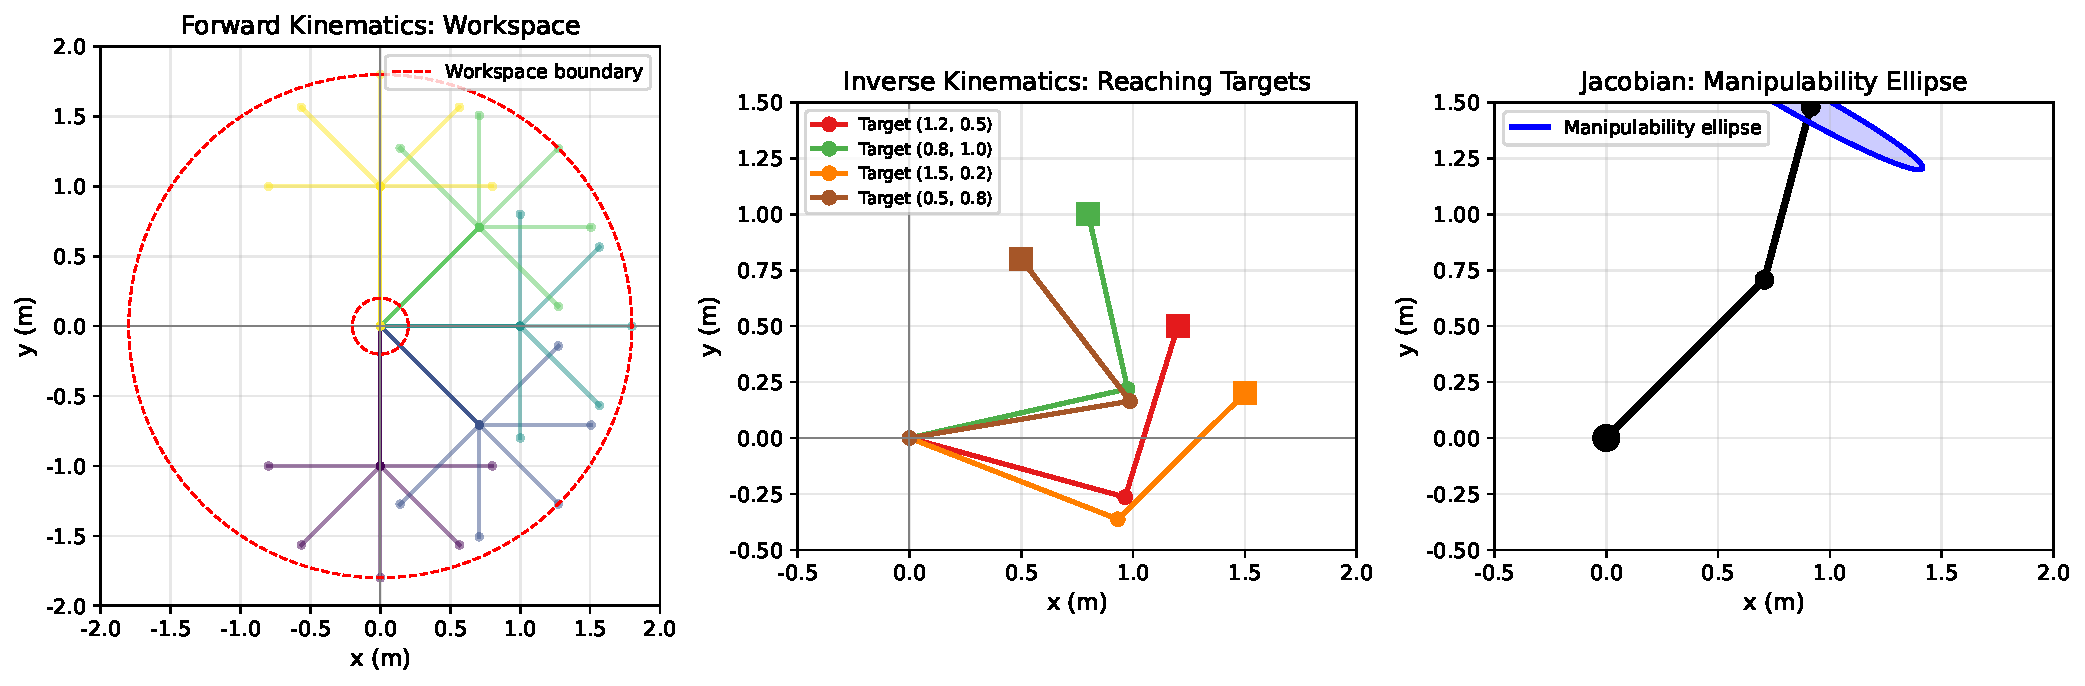
\includegraphics[width=0.95\textwidth]{figs_chap10/arm_kinematics.pdf}
\caption{二连杆机械臂运动学。左图：正运动学——给定关节角度，计算末端位置，扫出工作空间。中图：逆运动学——给定目标位置，求解关节角度。右图：雅可比矩阵决定的"可操作性椭圆"，反映不同方向上的运动能力。}
\label{fig:arm_kinematics}
\end{figure}

\paragraph{正运动学}
给定关节角度$(\theta_1, \theta_2)$，末端位置为：
\begin{align}
    x &= L_1 \cos\theta_1 + L_2 \cos(\theta_1 + \theta_2) \\
    y &= L_1 \sin\theta_1 + L_2 \sin(\theta_1 + \theta_2)
\end{align}

\paragraph{逆运动学}
给定目标位置$(x, y)$，需要求解$(\theta_1, \theta_2)$。这是一个非线性方程组，通常有多个解（对应不同的肘部朝向）。用余弦定理可得：
\[
\cos\theta_2 = \frac{x^2 + y^2 - L_1^2 - L_2^2}{2 L_1 L_2}
\]

\paragraph{雅可比矩阵}
末端速度与关节速度的关系由\textbf{雅可比矩阵}描述：
\[
\begin{pmatrix} \dot{x} \\ \dot{y} \end{pmatrix} = J(\theta) \begin{pmatrix} \dot{\theta}_1 \\ \dot{\theta}_2 \end{pmatrix}
\]

雅可比矩阵的奇异值分解揭示了机械臂在不同方向的"灵活度"——椭圆长轴方向容易运动，短轴方向难以运动。

% ------------------------------------------------------------------------------------
\subsection*{三、传统控制 vs 强化学习}

\begin{figure}[htbp]
\centering
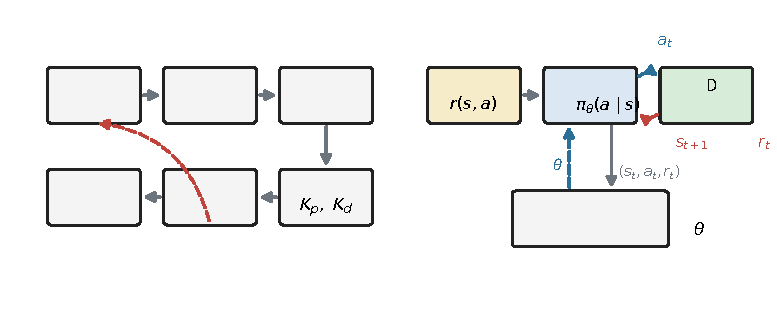
\includegraphics[width=0.95\textwidth]{figs_chap10/rl_control_comparison.pdf}
\caption{控制方法对比。传统控制需要精确建模、控制器设计、稳定性分析；强化学习只需定义奖励函数，让智能体在交互中学习，但需要大量训练样本和计算资源。}
\label{fig:rl_control_comparison}
\end{figure}

\paragraph{传统方法：PD控制}
最简单的控制策略是\textbf{PD控制器}：
\[
\tau = K_p (\theta_{\text{target}} - \theta) - K_d \dot{\theta}
\]

这需要：(1) 知道目标角度（需要逆运动学）；(2) 调节增益$K_p, K_d$；(3) 假设动力学足够简单。

图\ref{fig:pd_control}展示了PD控制器跟踪圆形轨迹的效果——在简单任务上表现良好，但对模型误差和外部扰动敏感。

\begin{figure}[htbp]
\centering
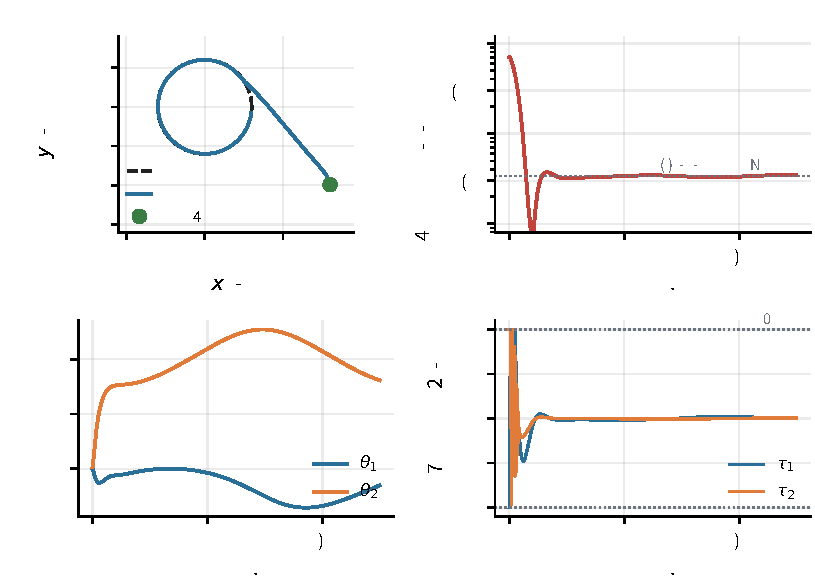
\includegraphics[width=0.95\textwidth]{figs_chap10/pd_control_trajectory.pdf}
\caption{PD控制器跟踪圆形轨迹。左上：末端实际轨迹vs目标轨迹。右上：跟踪误差。左下：关节角度随时间变化。右下：控制力矩。}
\label{fig:pd_control}
\end{figure}

\paragraph{强化学习方法}
RL不需要显式的逆运动学或动力学模型。智能体直接学习从状态到力矩的映射：
\[
\pi_\theta: (\theta_1, \theta_2, \dot{\theta}_1, \dot{\theta}_2, x_{\text{goal}}, y_{\text{goal}}) \mapsto (\tau_1, \tau_2)
\]

奖励设计示例：
\[
r = -\|p_{\text{end}} - p_{\text{goal}}\|^2 - 0.01 \|\tau\|^2
\]
第一项鼓励接近目标，第二项惩罚过大的力矩。

% ------------------------------------------------------------------------------------
\subsection*{四、CartPole：连续控制的入门任务}

在动手实现机械臂RL之前，先用更简单的\textbf{CartPole}任务热身（图\ref{fig:cartpole_demo}）。

\begin{figure}[htbp]
\centering
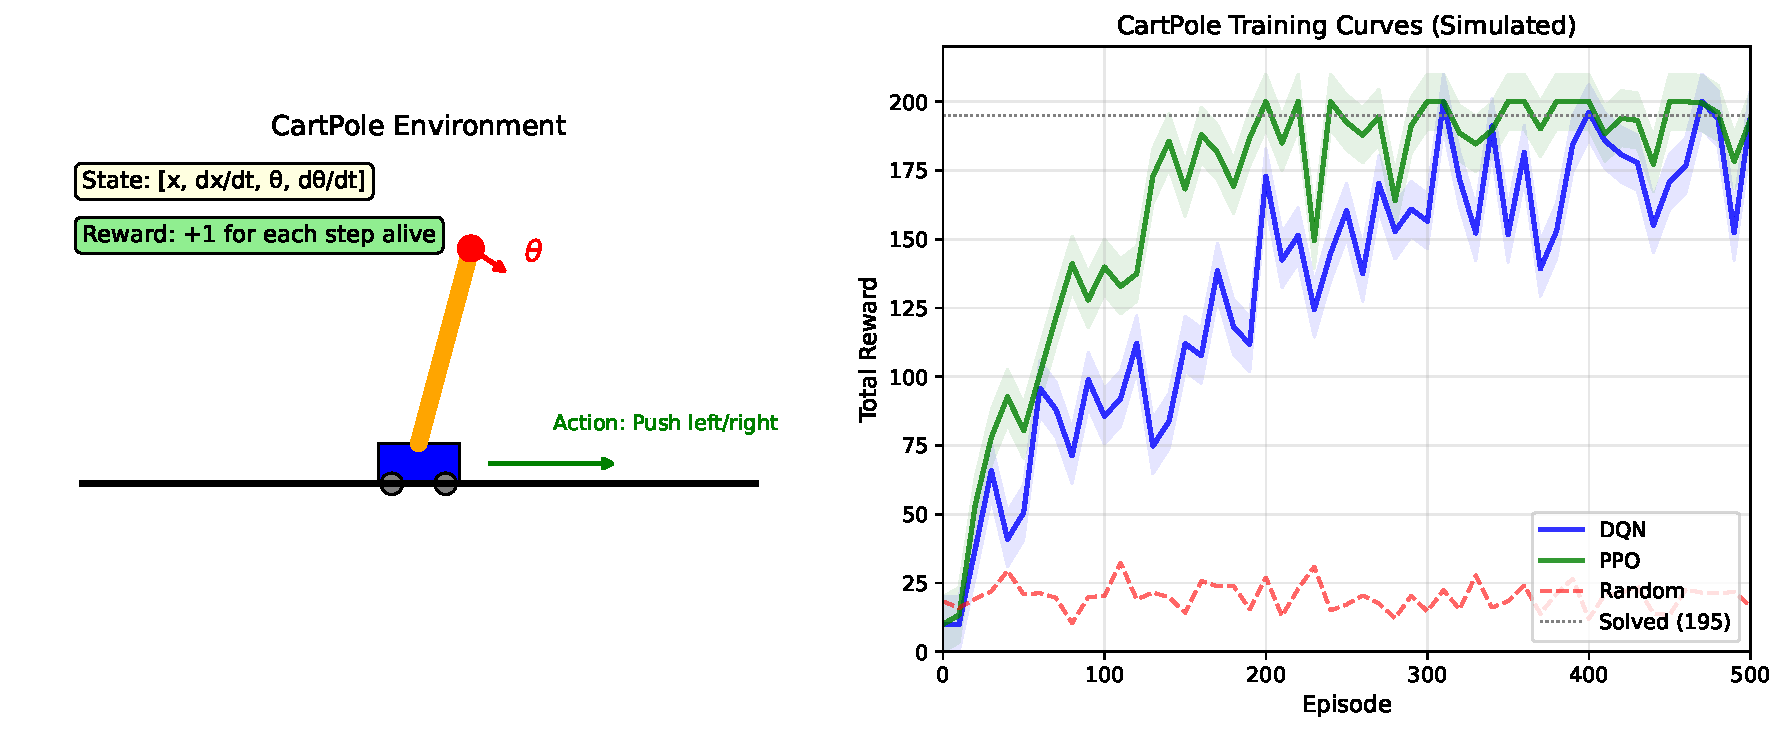
\includegraphics[width=0.95\textwidth]{figs_chap10/cartpole_demo.pdf}
\caption{CartPole任务。左图：环境示意——小车上竖立一根杆，目标是通过左右推动小车让杆保持竖直。状态是4维连续向量，动作是离散的（左/右）。右图：不同算法的学习曲线（模拟）——PPO和DQN都能在几百个episode内学会，随机策略则始终徘徊在低奖励。}
\label{fig:cartpole_demo}
\end{figure}

CartPole的状态是4维向量$[x, \dot{x}, \theta, \dot{\theta}]$，目标是让杆保持竖直（$|\theta| < 12°$）且小车不出界（$|x| < 2.4$）。每坚持一步获得+1奖励，达到200步"solved"。

\paragraph{用Stable Baselines3训练}

\begin{lstlisting}[language=Python]
import gymnasium as gym
from stable_baselines3 import PPO

# 创建环境
env = gym.make("CartPole-v1")

# 创建并训练智能体
model = PPO("MlpPolicy", env, verbose=1)
model.learn(total_timesteps=50000)

# 测试
obs, _ = env.reset()
for _ in range(200):
    action, _ = model.predict(obs, deterministic=True)
    obs, reward, done, truncated, info = env.step(action)
    if done:
        break
\end{lstlisting}

PPO（Proximal Policy Optimization）是目前最常用的策略梯度算法，在ChatGPT的RLHF训练中也使用了它。

% ------------------------------------------------------------------------------------
\subsection*{五、进阶：用RL控制机械臂}

机械臂控制比CartPole复杂得多：
\begin{itemize}
    \item 动作空间是\textbf{连续}的（力矩值），需要用SAC或TD3等算法
    \item 状态维度更高（关节+目标位置）
    \item 奖励设计更关键（稀疏奖励很难学习）
\end{itemize}

推荐使用\texttt{gymnasium-robotics}库中的\texttt{FetchReach}等环境，或者MuJoCo物理引擎中的机械臂任务。

\begin{lstlisting}[language=Python]
import gymnasium as gym
from stable_baselines3 import SAC

# 机械臂到达任务（需要安装gymnasium-robotics）
env = gym.make("FetchReach-v3")

# SAC适合连续动作空间
model = SAC("MultiInputPolicy", env, verbose=1)
model.learn(total_timesteps=100000)
\end{lstlisting}

% ------------------------------------------------------------------------------------
\subsection*{六、实践建议}

\begin{insightbox}[title=连续控制学习路线]
\begin{enumerate}
    \item \textbf{入门}：CartPole + DQN/PPO，理解基本训练流程
    \item \textbf{进阶}：Pendulum/MountainCarContinuous + SAC，体验连续动作空间
    \item \textbf{挑战}：FetchReach/HalfCheetah，接触真实机器人仿真
    \item \textbf{实战}：sim-to-real迁移，将仿真策略部署到真实机器人
\end{enumerate}
\end{insightbox}

完整代码见\texttt{code\_chap10/robotic\_arm\_control.py}。

\begin{remark}
从GridWorld到机械臂，我们看到了强化学习的通用性：只要能定义状态、动作、奖励，同样的算法框架就能应用。但"能应用"不等于"好用"——连续控制的样本效率、奖励设计、sim-to-real差距都是活跃的研究方向。
\end{remark}
